

\onecolumn

\section{Proof of Theorem \ref{thm:revolver}} \label{sec:thm:proof}


Since $E(\cdot)$ is a continuous function of robot models, we assume the transition dynamics of the robot $E(\alpha)$ is differentiable and locally $L_1$-Lipschitz w.r.t. $\alpha$ in the sense that
\begin{equation}\label{eq:alpha:lipschitz:assumption}
\begin{split}
     \exists \varepsilon > 0,
    ||E(\alpha)(s,a) - E(\alpha^\prime)(s,a)|| \le L_1 |\alpha - \alpha^\prime|, 
    \forall s\in\mathcal{S}, \forall a\in\mathcal{A}, \forall |\alpha^\prime - \alpha | < \varepsilon    
\end{split}
\end{equation}
Moreover, we follow \cite{slbo} and assume the value functions of the robot models are $L_2$-Lipschitz w.r.t to some norm $||\cdot||$ in state space in the sense that
\begin{equation}\label{eq:state:lipschitz:assumption}
    |V^{\pi, M}(s) - V^{\pi, M}(s^\prime)| \le L_2 ||s-s^\prime||, \forall s, s^\prime \in \mathcal{S}
\end{equation}


By the assumption in Equation \eqref{eq:state:lipschitz:assumption} that the value functions of the robots are $L_2$-Lipschitz, as proven in Lemma 4.1 of \cite{slbo}, $\forall \phi > 0$, $M=E(\alpha), M^\prime=E(\alpha+\phi)$, we have 
\begin{equation}\label{eq:proof2}
\begin{split}
\exists \varepsilon > 0, \text{s.t. }
\mathop{\mathbb{E}}_{s} [ |V^{\pi,M}(s) - V^{\pi,M^\prime}(s)| ] 
& \le \frac{\gamma}{1-\gamma} L_2 \mathop{\mathbb{E}}_{(s,a)\sim \pi} || M(s,a) - M^\prime(s,a) || \\
& = \frac{\gamma}{1-\gamma} L_2 \mathop{\mathbb{E}}_{(s,a)\sim \pi} || E(\alpha)(s,a) - E(\alpha^\prime)(s,a) || \\
& \le \frac{\gamma}{1-\gamma} L_2 L_1 |\alpha - \alpha^\prime|, \forall |\alpha^\prime - \alpha | < \varepsilon 
\end{split}
\end{equation}
Since the value functions are differentiable by assumption in Equation \eqref{eq:alpha:lipschitz:assumption}, suppose $D = | \frac{\partial{V^{\pi,E(\alpha)}}}{\alpha} | $ is the absolute value of the derivative of $V^{\pi,E(\alpha)}$ w.r.t. to $\alpha$. 
According to Equation \eqref{eq:proof2}, $D$ is bounded.
We make a (strong) assumption that for all $\varphi\in [\alpha, \alpha+\xi]$, policy $\pi^*_{E(\varphi)}$ only achieves the best expected reward on robot $E(\varphi)$, so that
\begin{equation}
    \forall \varphi, \beta \in [\alpha, \alpha+\xi], 
    V^{\pi^*_{E(\varphi)},E(\varphi)} -
    V^{\pi^*_{E(\varphi)},E(\beta)} = D \cdot |\varphi - \beta| + o(|\beta-\varphi|^2)
    = D \cdot |\varphi - \beta| + o(\xi^2)
\end{equation}
From the definition, the value function of a policy $\pi$ on uniformly sampled robots $E(\beta)$ from $\beta\sim U(\alpha, \alpha+\xi)$ is
\begin{equation}
\begin{split}\label{eq:proof1}
    & \mathop{\mathbb{E}}_{ 
    \substack{
    \beta \sim U(\alpha, \alpha+\xi)
    }}
    \mathop{\mathbb{E}}_{ 
    \substack{(s_t, a_t) \sim \pi, E(\beta)
    }}
    \sum_{t} \gamma^t r_t \cdot\exp(h\beta) \\
    = & \mathop{\mathbb{E}}_{ 
    \substack{
    \beta \sim U(\alpha, \alpha+\xi)
    }}
    \exp(h\beta)
    \mathop{\mathbb{E}}_{ 
    \substack{(s_t, a_t) \sim \pi, E(\beta)
    }}
    \sum_{t} \gamma^t r_t  \\ 
    = & \mathop{\mathbb{E}}_{ 
    \substack{
    \beta \sim U(\alpha, \alpha+\xi)
    }}
    \exp(h\beta)
    V^{\pi,E(\beta)}  \\
    = & \frac{1}{\xi} \int_{\beta=\alpha}^{\alpha+\xi} \exp(h\beta)
    V^{\pi,E(\beta)} \dd{\beta}
\end{split}
\end{equation}
Supposed the $\pi$ that optimizes Equation \eqref{eq:proof1} is the policy that directly optimizes on one robot $E(\varphi), \varphi \in [\alpha, \alpha+\xi]$, i.e. $\pi^*_{E(\varphi)}$ optimizes Equation \eqref{eq:proof1}, then we treat $\pi^*_{E(\varphi)}$ and $V^{\pi^*_{E(\varphi)},E(\varphi)}$ as constants and the following variation should be zero
\begin{equation}
\begin{split}
    \delta \int_{\beta=\alpha}^{\alpha+\xi} \exp(h\beta)
    (V^{\pi^*_{E(\varphi)},E(\beta)} - V^{\pi^*_{E(\varphi)},E(\varphi)})  \dd{\beta} = 0
\end{split}
\end{equation}
which means
\begin{equation}
\begin{split}
    0 = & \int_{\beta=\alpha}^{\alpha+\xi} \frac{\partial}{\partial \beta} [ \exp(h\beta)
    (V^{\pi^*_{E(\varphi)},E(\beta)} - V^{\pi^*_{E(\varphi)},E(\varphi)}) ]  \dd{\beta}  \\ 
    \approx & \int_{\beta=\alpha}^{\varphi} \frac{\partial}{\partial \beta} [\exp(h\beta) D |\varphi-\beta| ] \dd{\beta} - \int_{\beta=\varphi}^{\alpha+\xi} \frac{\partial}{\partial \beta} [\exp(h\beta) D |\varphi-\beta| ] \dd{\beta} + o(\xi^2) \\
    = & D \int_{\beta=\alpha}^{\varphi} \frac{\partial}{\partial \beta} [\exp(h\beta) (\varphi - \beta) ] \dd{\beta} - D \int_{\beta=\varphi}^{\alpha+\xi} \frac{\partial}{\partial \beta} [\exp(h\beta) (\beta - \varphi) ] \dd{\beta} + o(\xi^2) \\
    = & \frac{e^{h\alpha}}{h} D [(h\varphi-1)(2e^{h(\varphi-\alpha)} - 1 - e^{h\xi}) + \\ & h(\alpha+\xi)e^{h\xi} - e^{h\xi} - h\varphi e^{h(\varphi-\alpha)} + e^{h(\varphi-\alpha)} - h\varphi e^{h(\varphi-\alpha)} + e^{h(\varphi-\alpha)} + h\alpha - 1 ] + o(\xi^2) \\
    = & \frac{e^{h\alpha}}{2h} D [(\alpha h^{2} \xi^{2} + 2 \alpha h \xi + 4 \alpha  + 2 h \xi^{2}  + 2 \xi) - (h^{2} \xi^{2} + 2 h \xi +4)\varphi ] +  o(\xi^2) 
\end{split}
\end{equation}
The last equation assumes $0 \le h(\varphi - \alpha) \le h\xi \ll 1$ and used second-order Taylor approximation of $e^y = 1 + y + \frac{1}{2}y^2 + o(y^2), y\in \mathbb{R}$. 
Then we have
\begin{equation}
\begin{split}
    \varphi & = \alpha + \frac{1}{2} \xi + \frac{\xi^2 h (2-\xi h)}{8 + 4\xi h + 2\xi^2 h^2} + o(\xi^2) \\
    & = \alpha + \frac{1}{2}\xi + \frac{1}{4} h\xi^2 + o(\xi^2)
\end{split}    
\end{equation}
Therefore, if
\begin{equation}
\begin{split}
    & \lim_{\xi \rightarrow 0}
    \left[
    \mathop{\arg\max}_{\pi}
    \mathop{\mathbb{E}}_{ 
    \substack{
    \beta \sim U(\alpha, \alpha + \xi) \\
    M_\beta = E(\beta)
    }}
    \mathop{\mathbb{E}}_{ 
    \substack{a_t \sim \pi(\cdot \mid s_t) \\ 
    s_{t+1} \sim M_\beta(\cdot \mid s_t, a_t)}}
    \sum_{t} \gamma^t r_t \exp(h \beta)
    \right] \\
    &
    = \pi_{M_\varphi}^* = \mathop{\arg\max}_{\pi}
    \mathop{\mathbb{E}}_{ 
    \substack{a_t \sim \pi(\cdot \mid s_t) \\ 
    s_{t+1} \sim M_\varphi(\cdot \mid s_t, a_t)}}
    \sum_{t} \gamma^t r_t,
\end{split}
\end{equation}
then when $\xi\rightarrow 0$, $\varphi = \alpha + \frac{1}{2}\xi + \frac{1}{4} h\xi^2 + o(\xi^2)$.
\qed






\section{Experiment Details}

\paragraph{ Caching Intermediate Robots  }
In practice, frequently calling the function for generating simulation environments could be costly.
To avoid repetitively generating a new environment at the start of every epoch and to speed up the training process, we pre-generate and cache a large number (e.g. 1,000) of environments.
At the start of each epoch, we randomly sample within the desired interpolation range and fetch a simulation environment from the cache.
When the number of cached environments is large, the above sampling behavior is a good approximation to sampling from continuous robot evolution.



\paragraph{Experiment Hyperparameter Setting}
We illustrate the hyperparameters of the neural networks used in Gym and Hand Manipulation Suite experiments, including layer size, batch size and learning rate, in Table \ref{tab:supp:net:param}.


\begin{table}[H]
\centering
\small
\begin{tabular}{l|c|c}
\hline
& MuJoCo Gym Environments & Hand Manipulation Suite \\
\hline
Actor & $[s,256,256,a]$ & $[s,32,32,a]$ \\ 
\hline
Critic & $[s+a,256,256,1]$ & $[s+a,32,32,1]$ \\ 
\hline
Batch size & 256 & 16 \\ 
\hline
Learning Rate & $3\times 10^{-4}$ & $1\times 10^{-4}$ \\
\hline
\end{tabular}
\vspace{-1ex}
\caption{Size of the Neural network used in the experiments. 
$s$ and $a$ represents the dimension of state space and action space respectively.
}
\label{tab:supp:net:param}
\end{table}




\section{Qualitative Results}

We show the process of transferring policy on intermediate robots on Hand Manipulation Suite tasks in Figure \ref{fig:dapg:evolve:viz}.
We show the transferred policy on the target robot of Hand Manipulation Suite tasks in Figure \ref{fig:dapg:policy:viz}. 
For more details, please refer to the supplementary video.


\begin{figure}[ht]
\centering
\newcommand\suppwidth{0.15}
\begin{tabular}{cccccc}
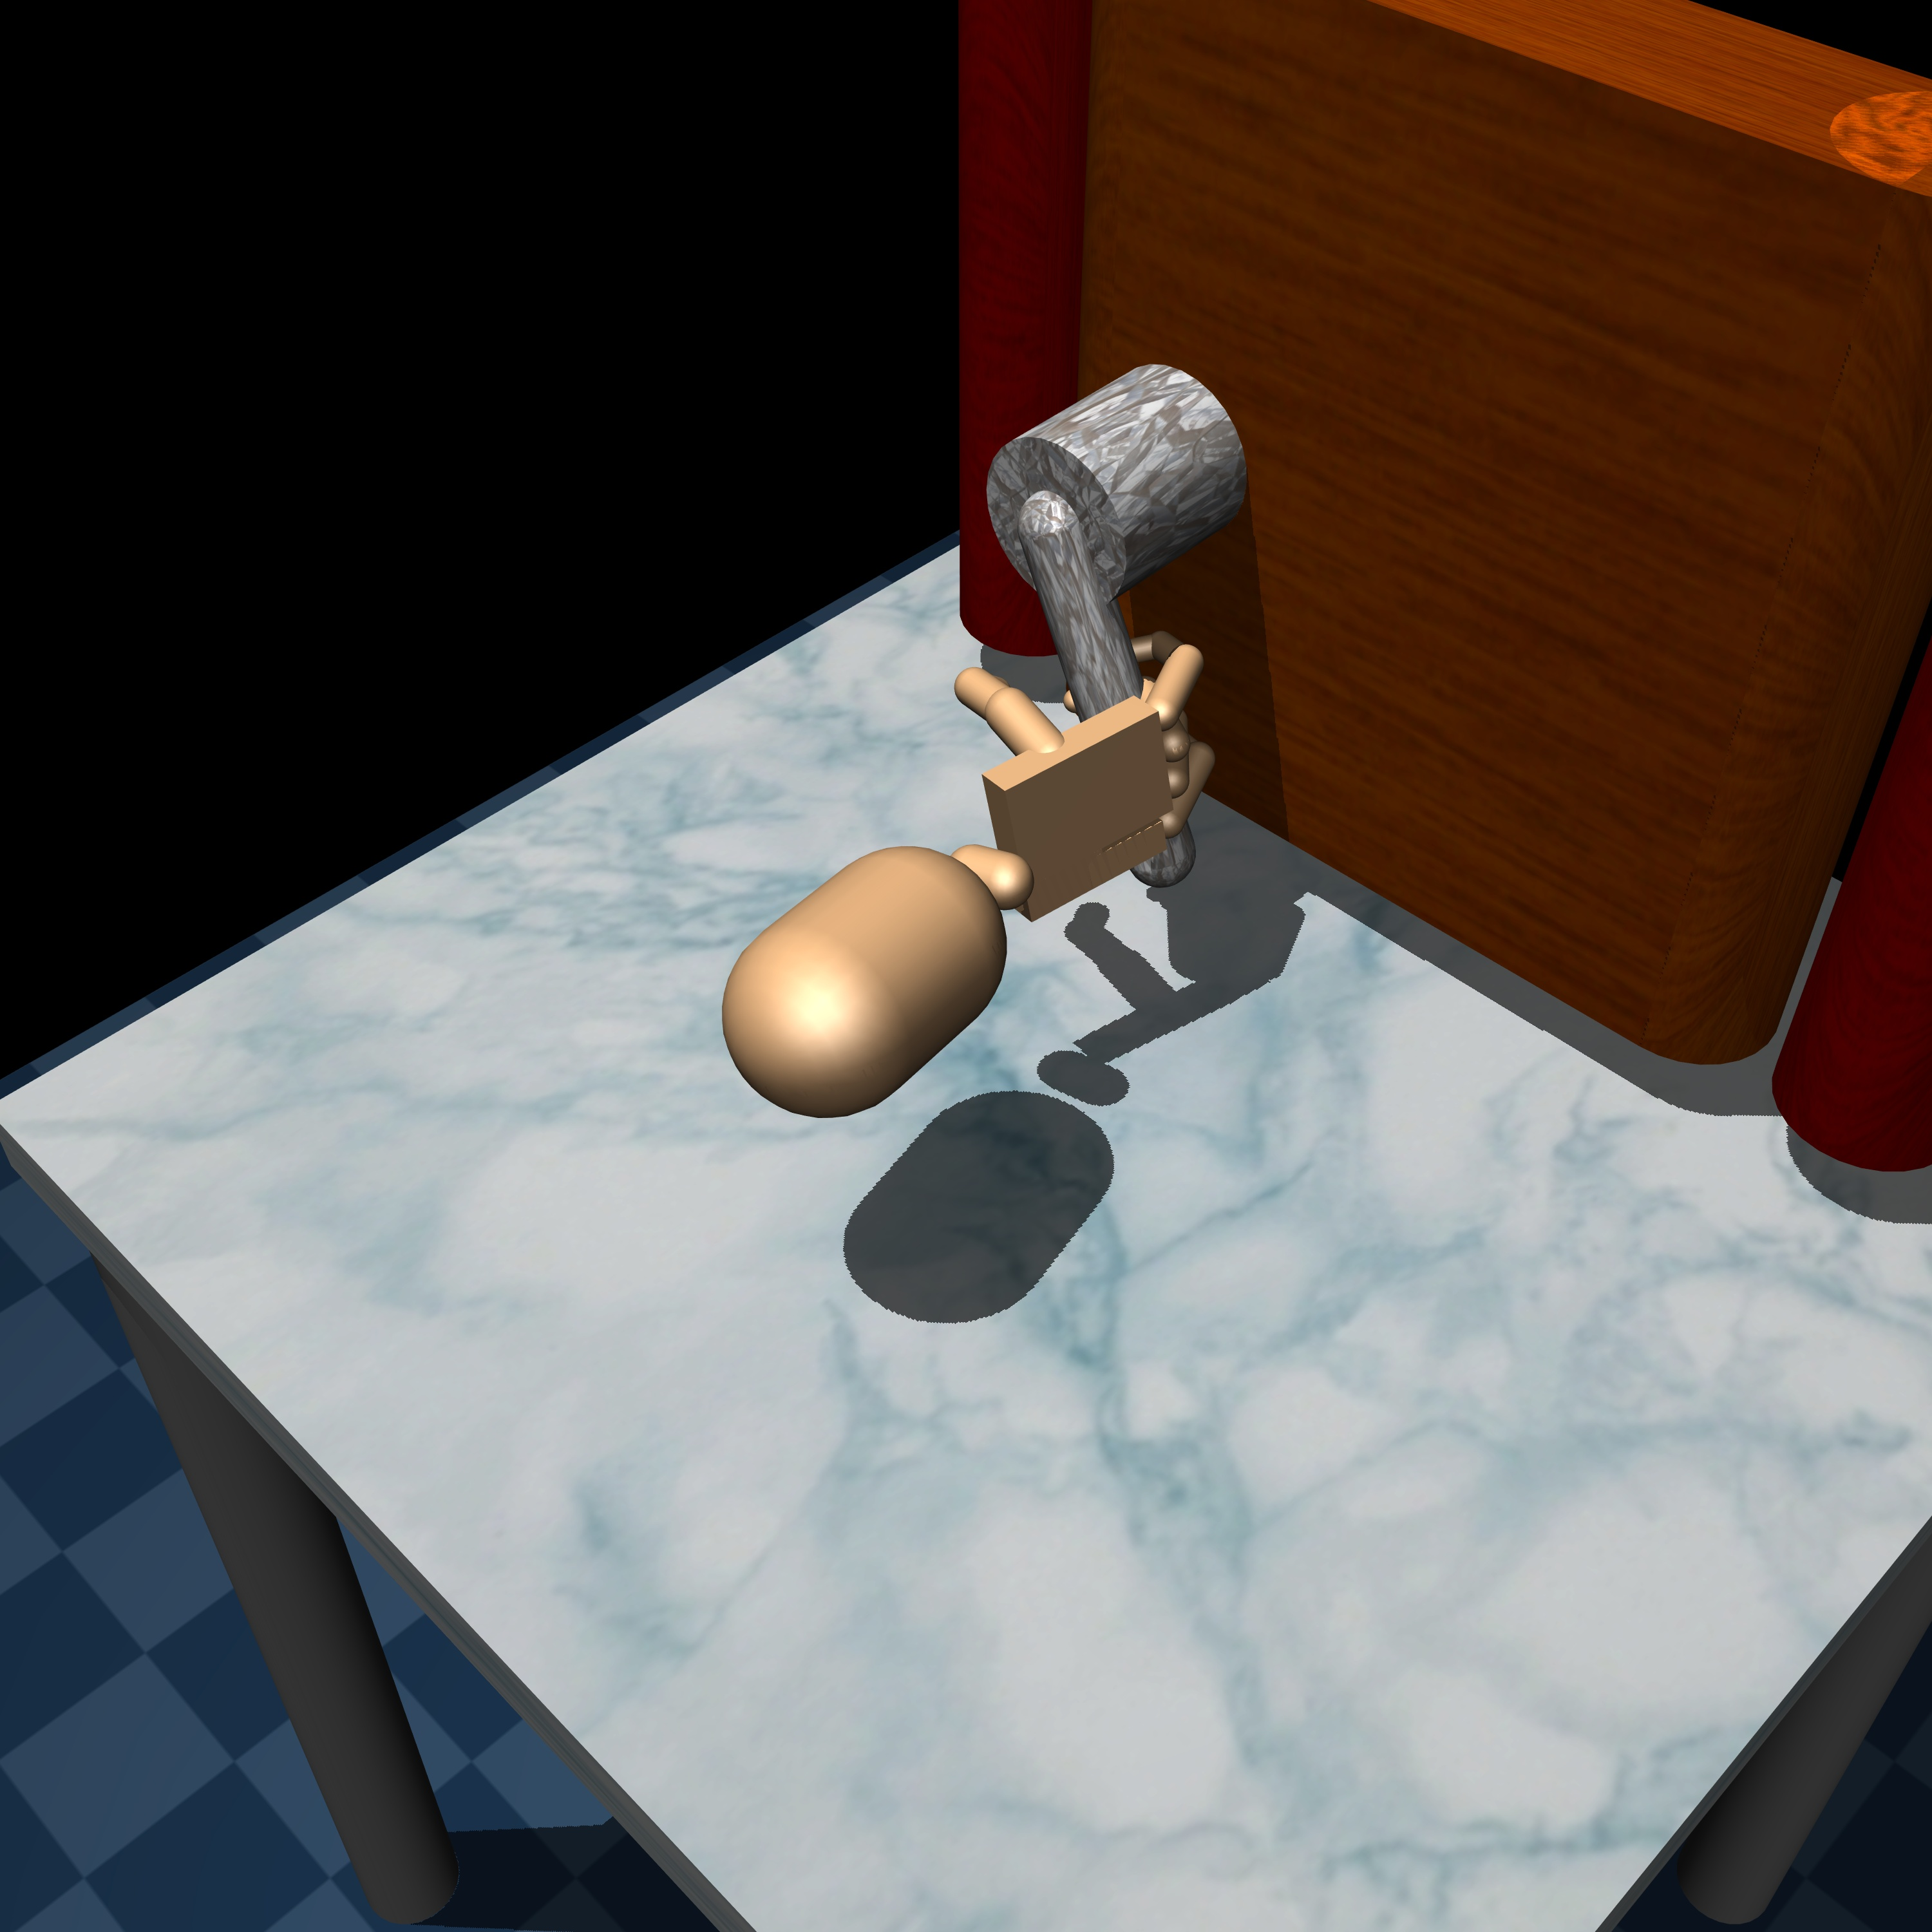
\includegraphics[width=\suppwidth\textwidth,valign=m]{Figures/supp/door/evolve/interp_0.0_image-0023.jpg}
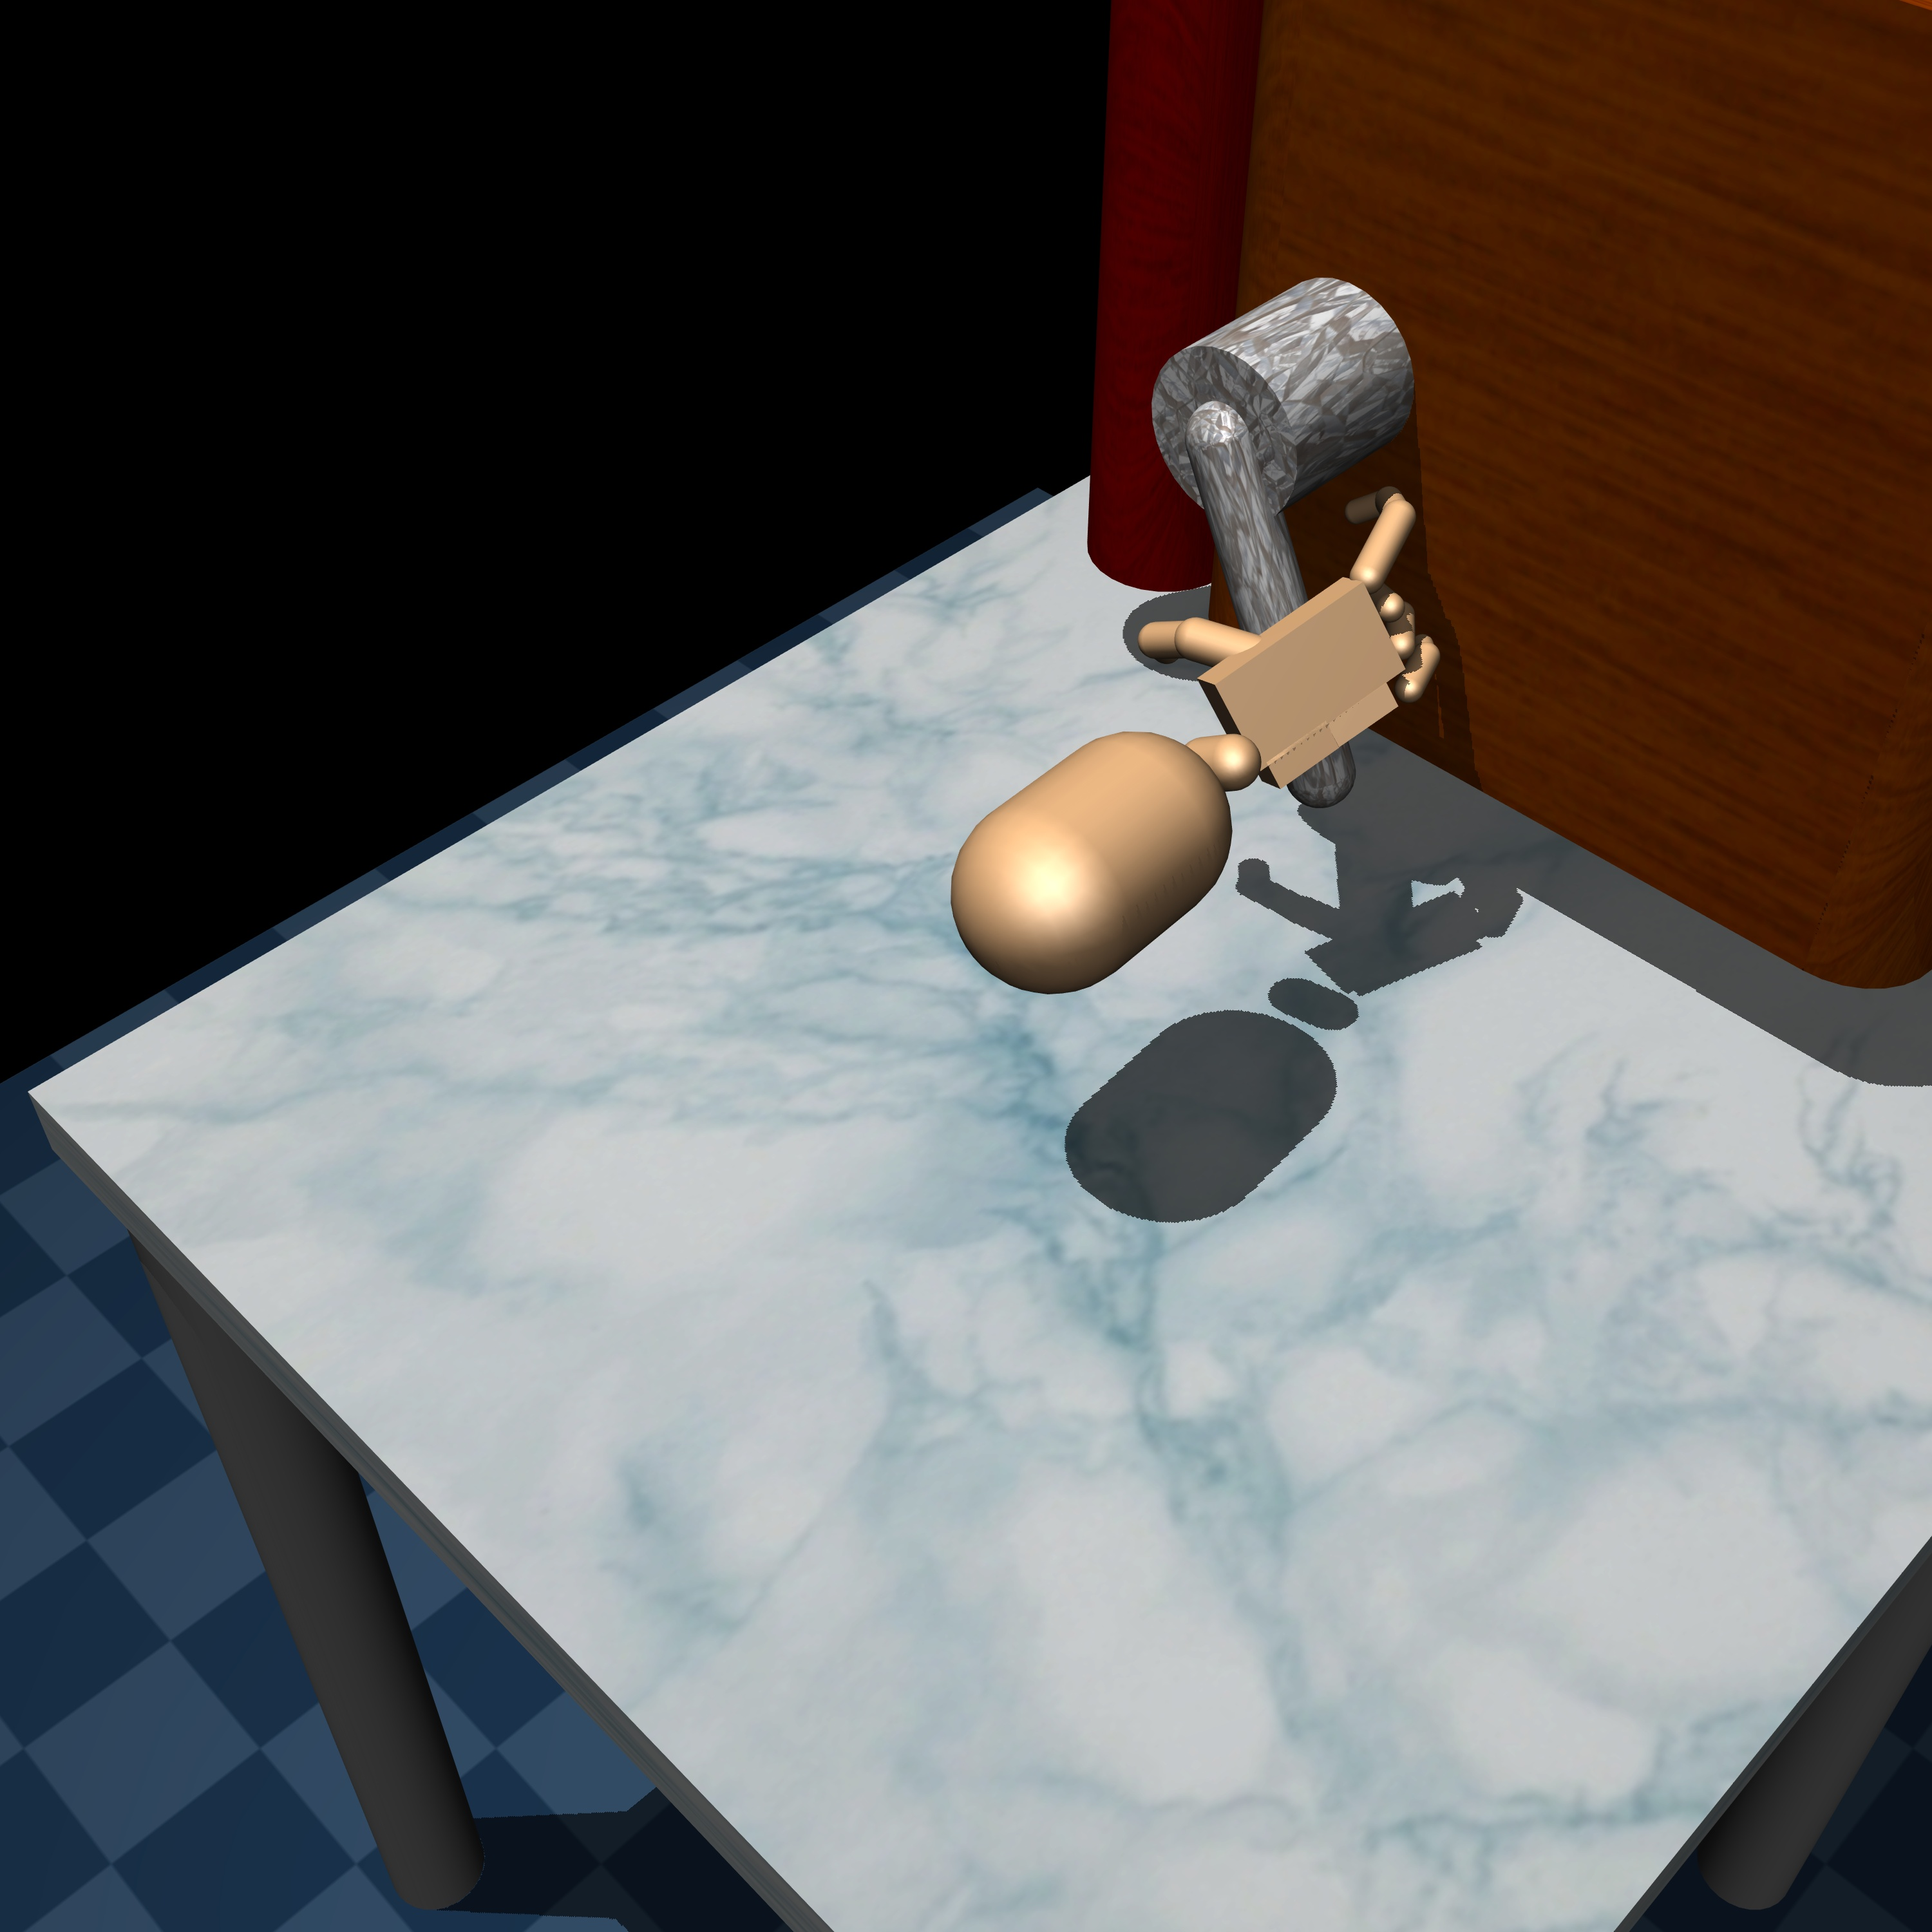
\includegraphics[width=\suppwidth\textwidth,valign=m]{Figures/supp/door/evolve/interp_0.2_image-0023.jpg}
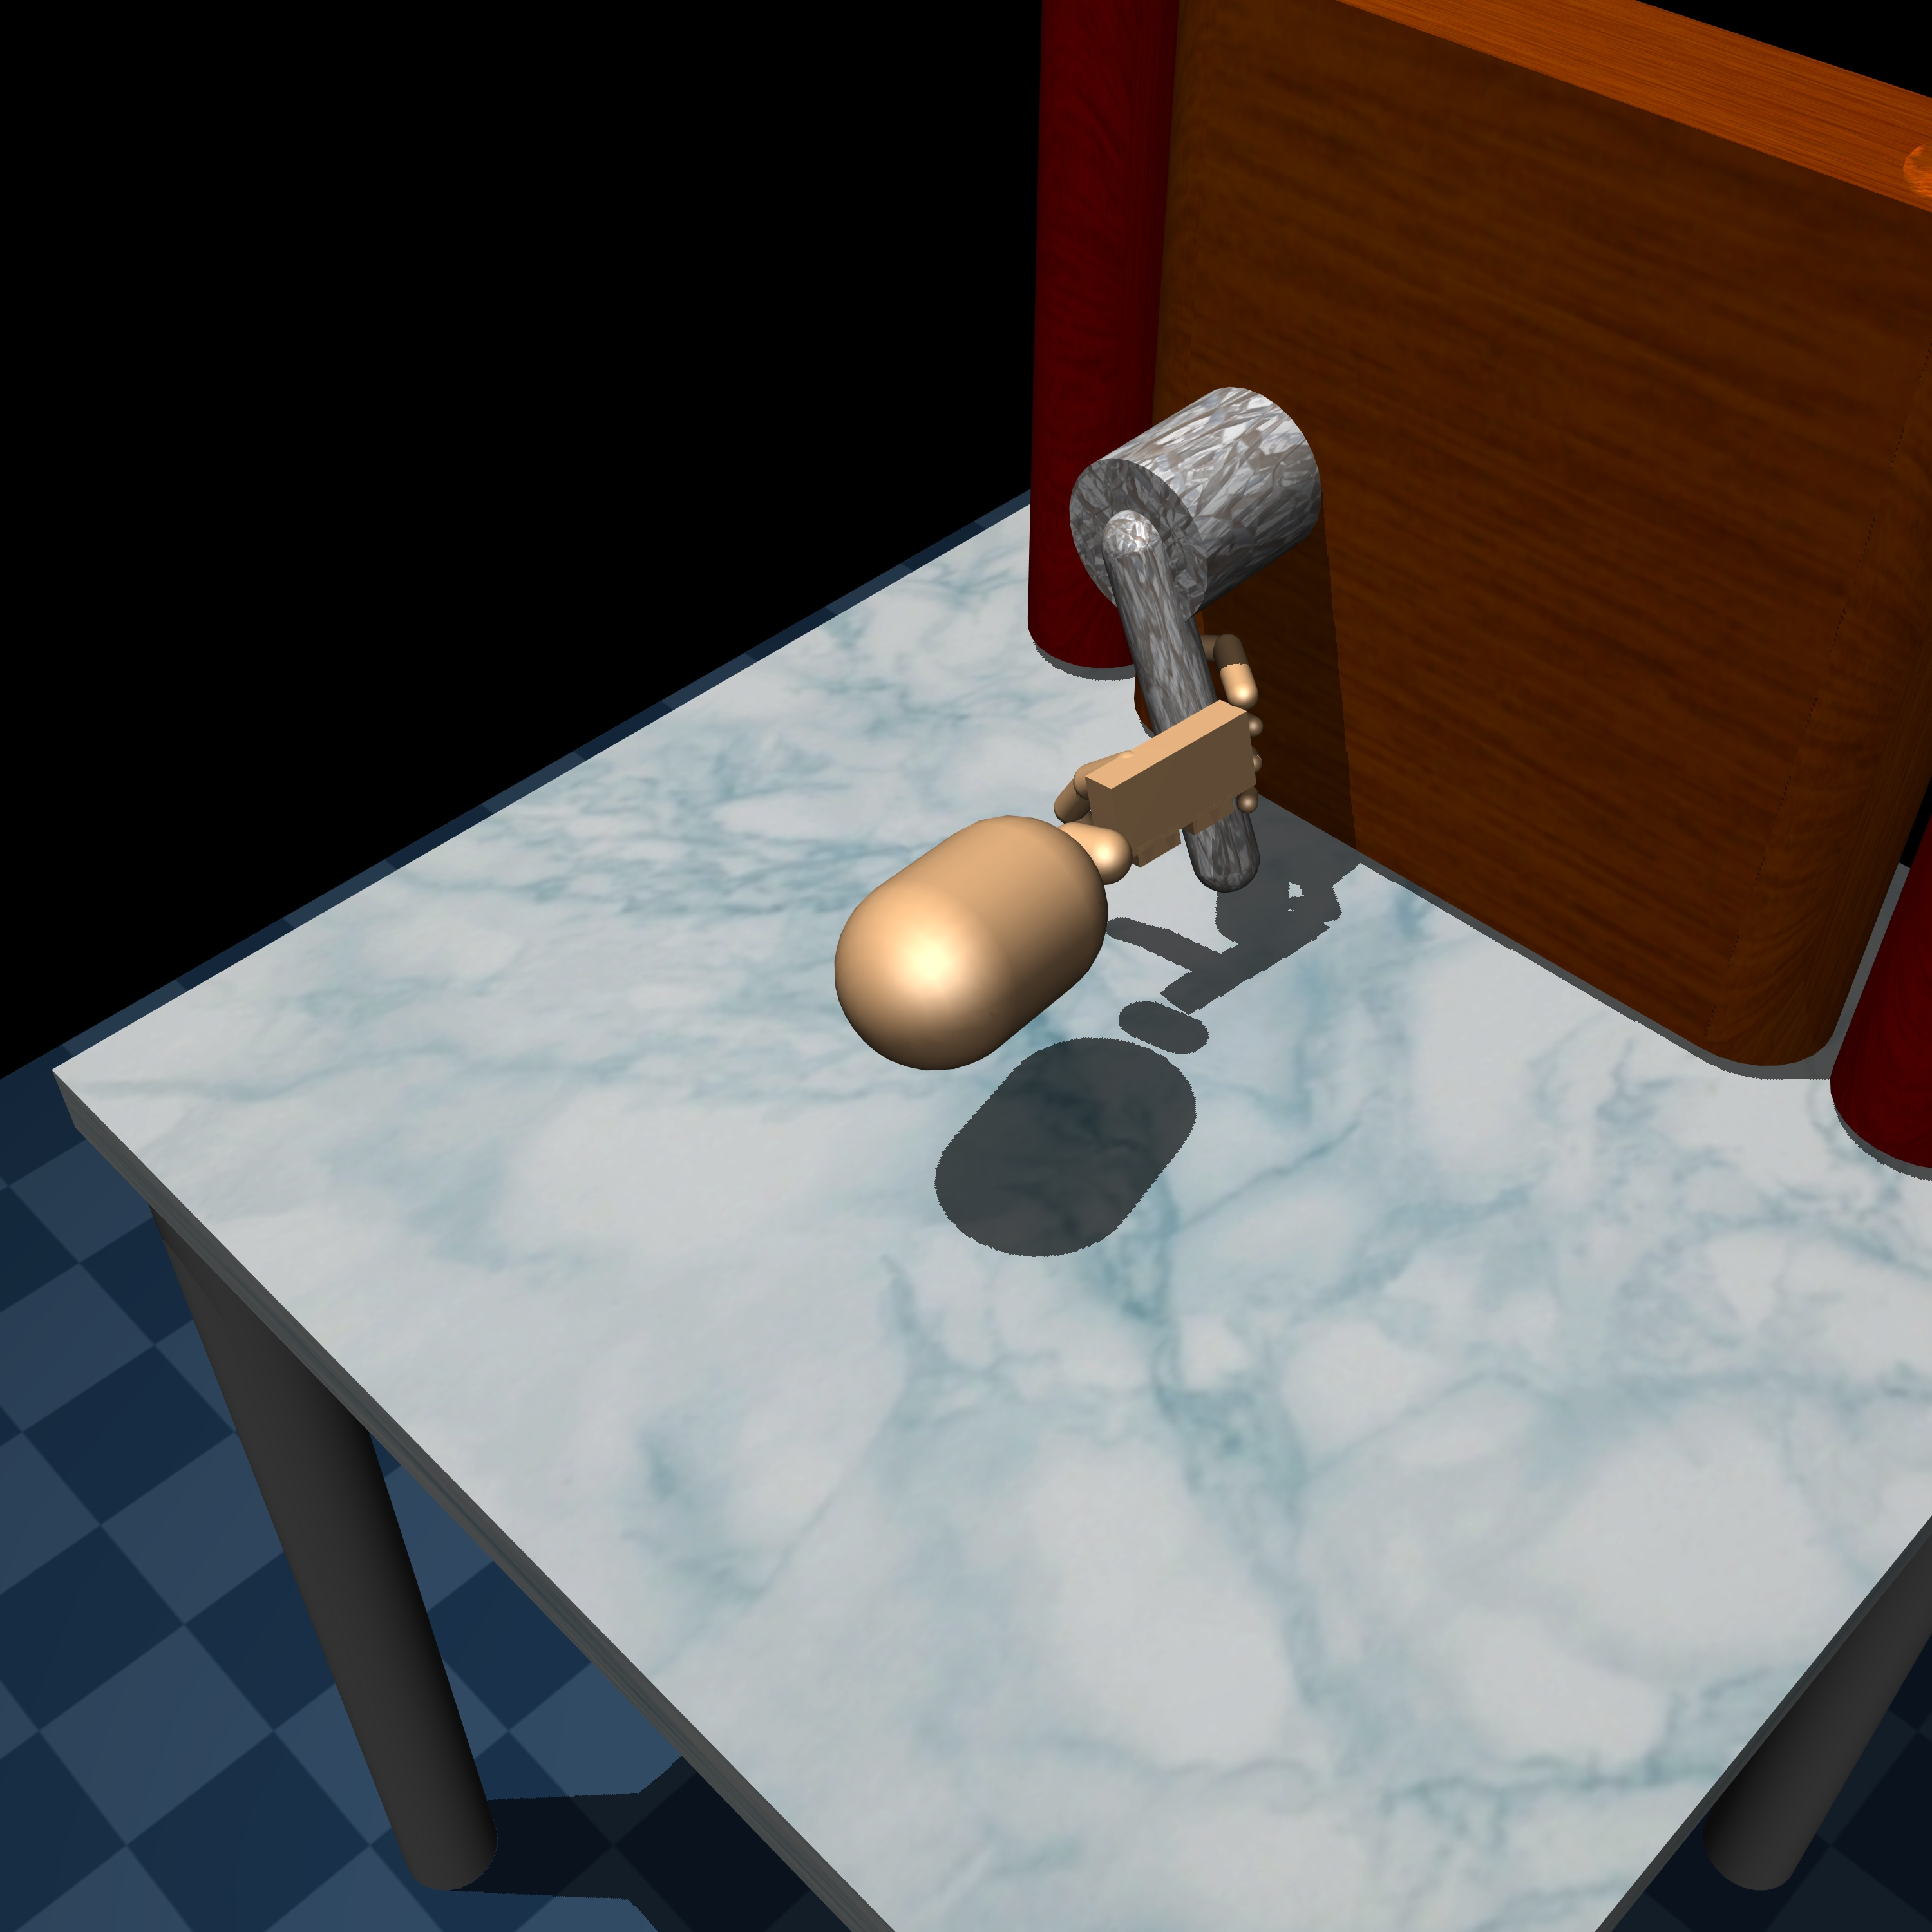
\includegraphics[width=\suppwidth\textwidth,valign=m]{Figures/supp/door/evolve/interp_0.4_image-0024.jpg}
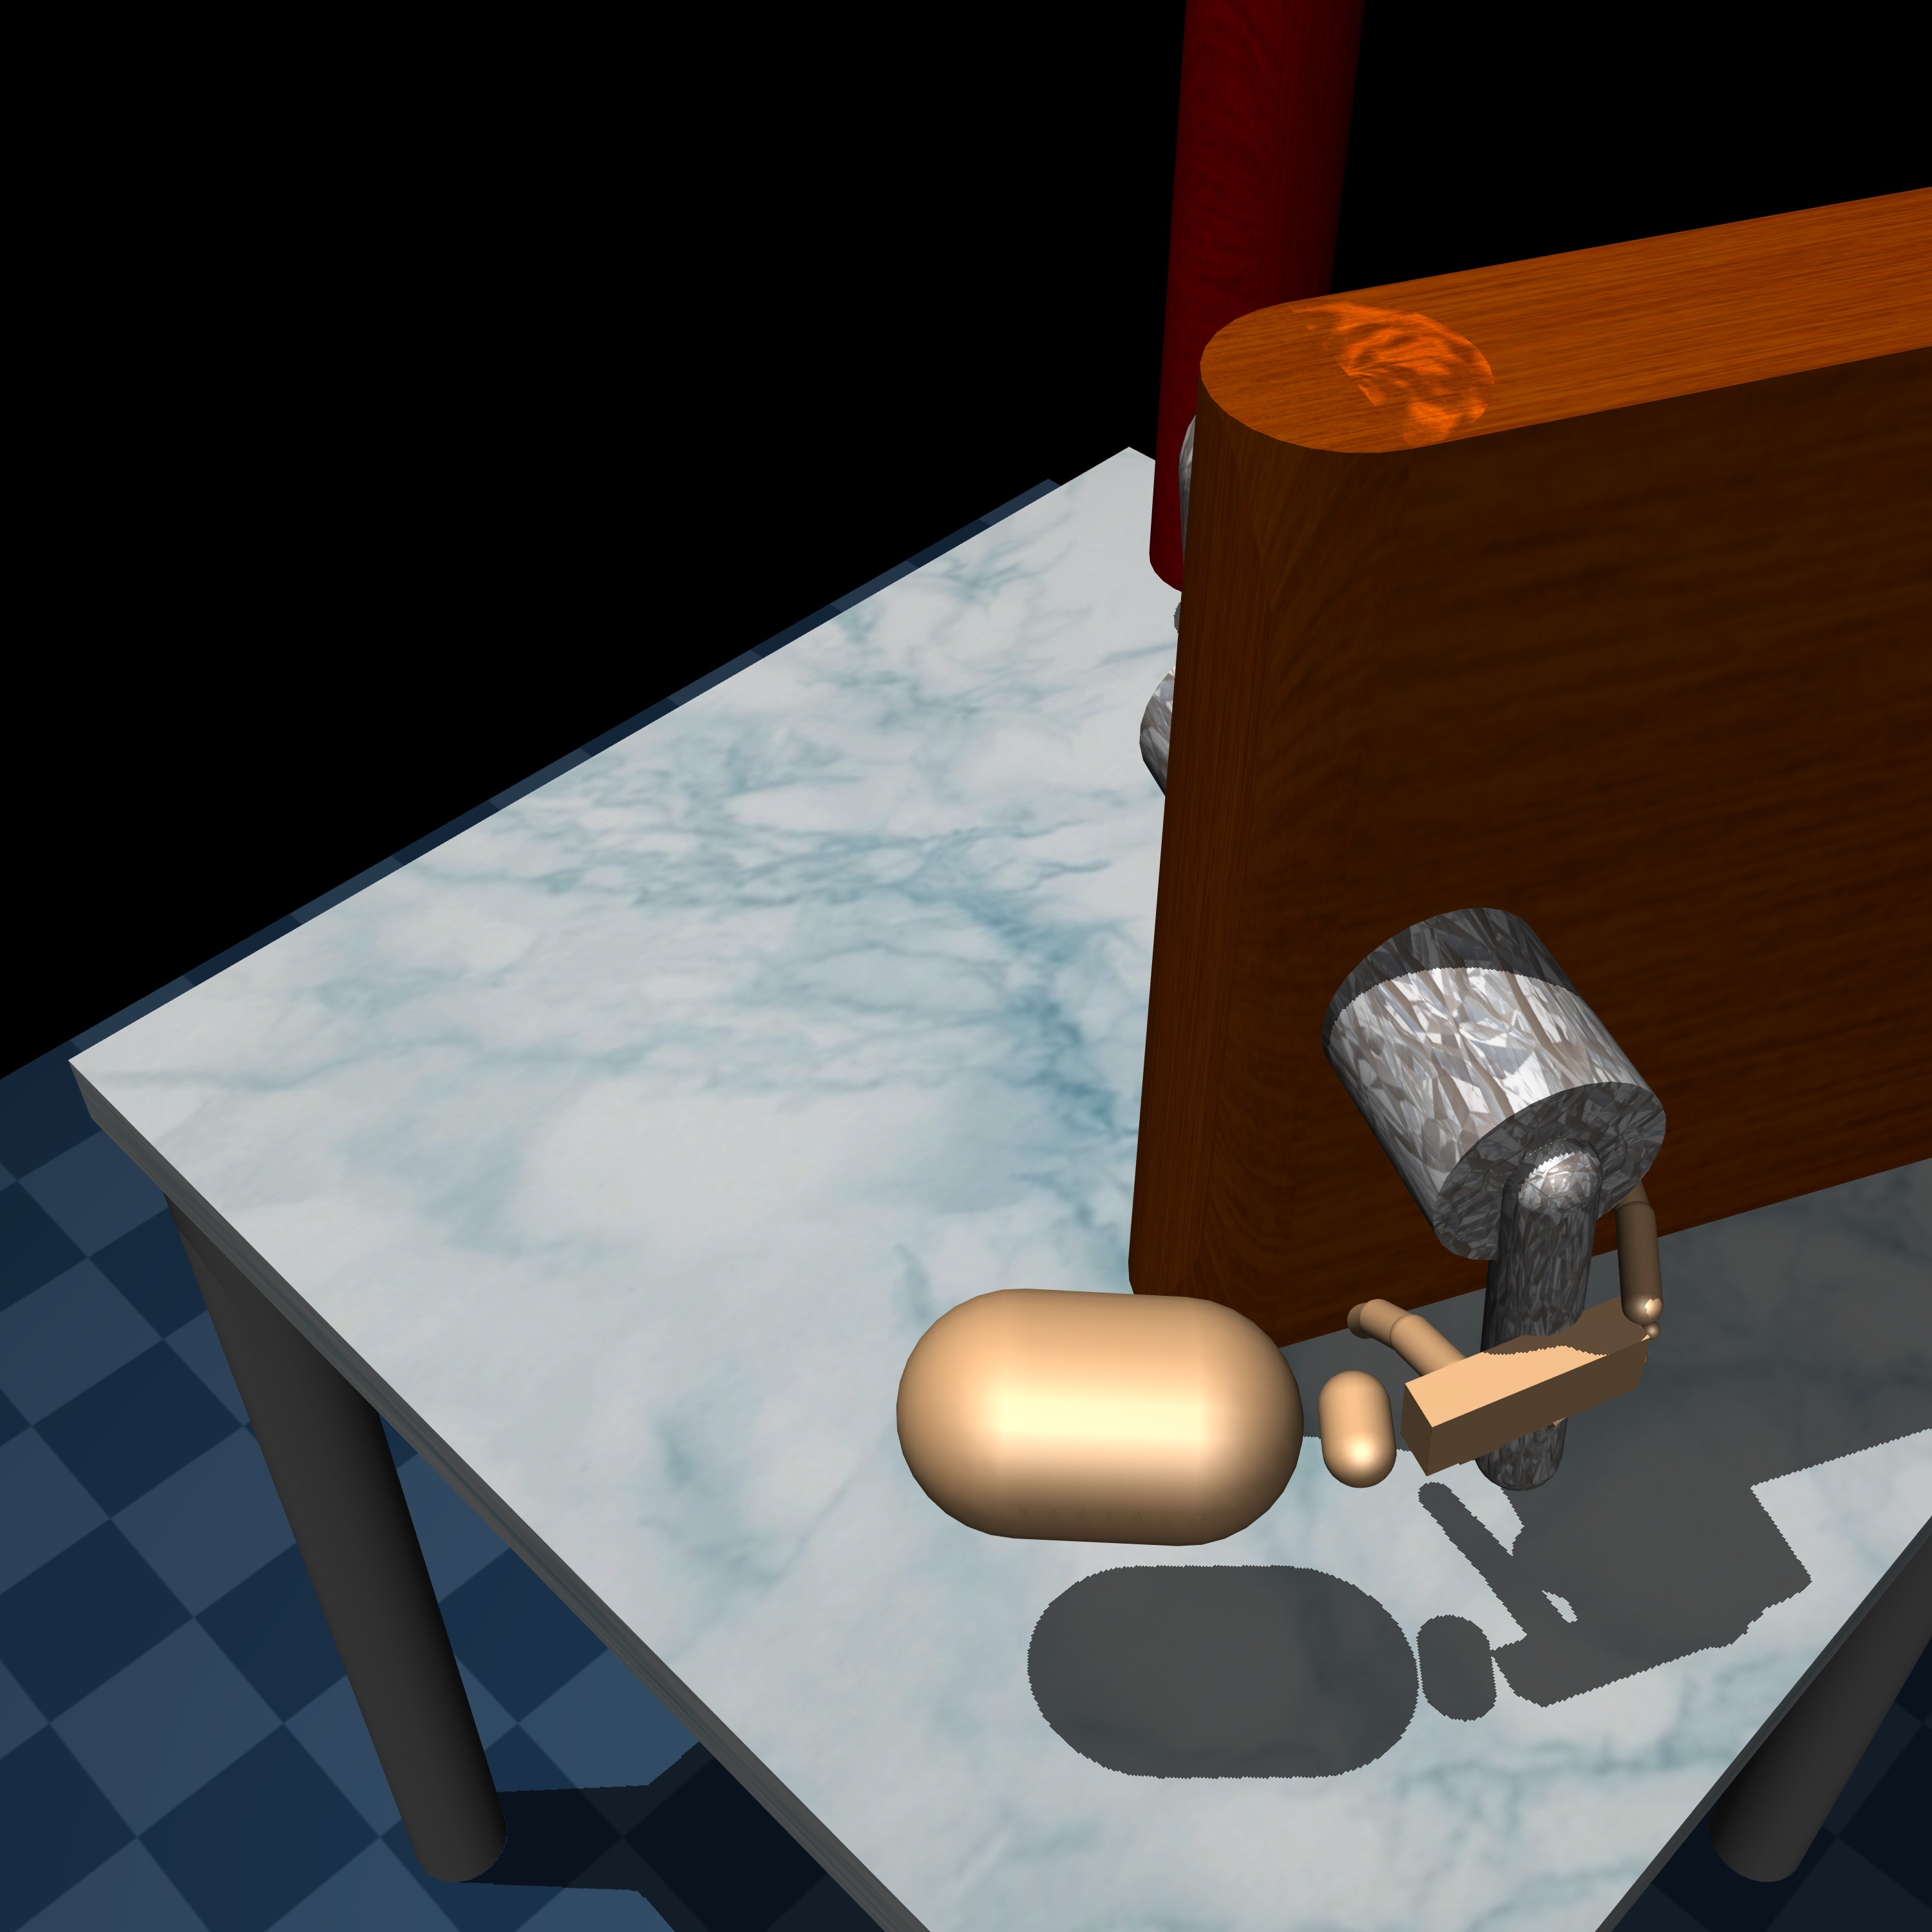
\includegraphics[width=\suppwidth\textwidth,valign=m]{Figures/supp/door/evolve/interp_0.6_image-0063.jpg}
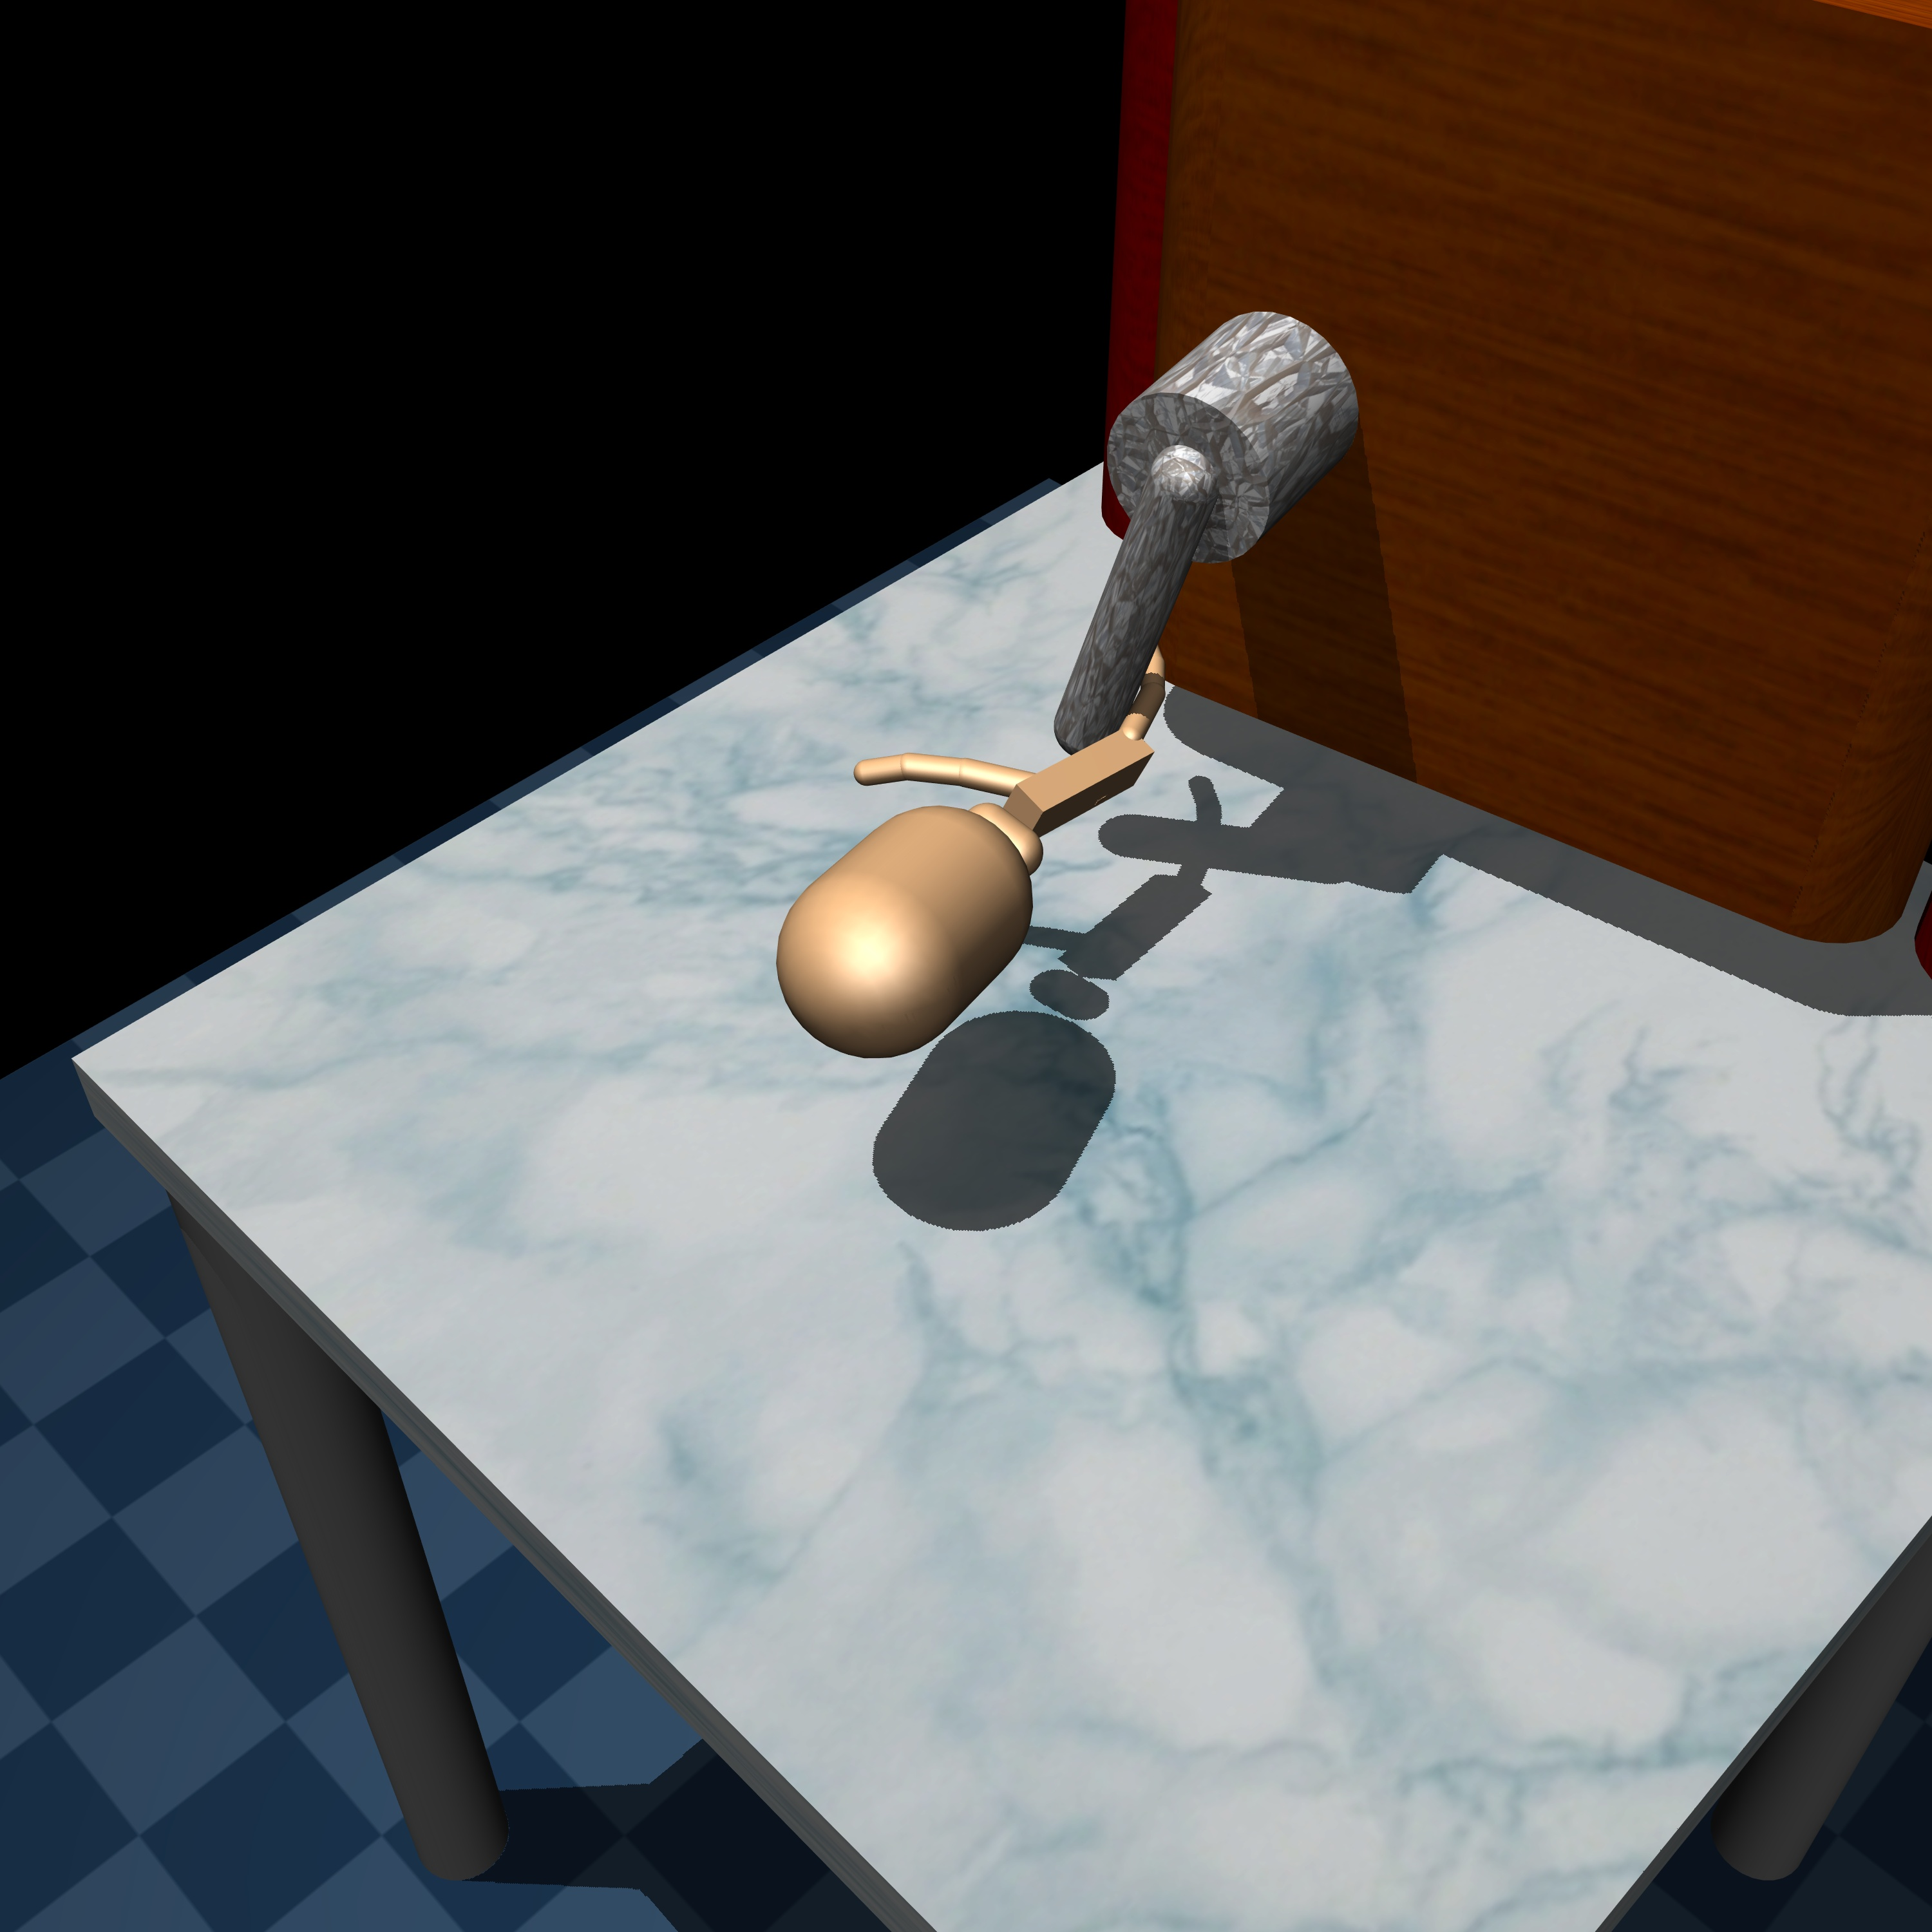
\includegraphics[width=\suppwidth\textwidth,valign=m]{Figures/supp/door/evolve/interp_0.8_image-0038.jpg}
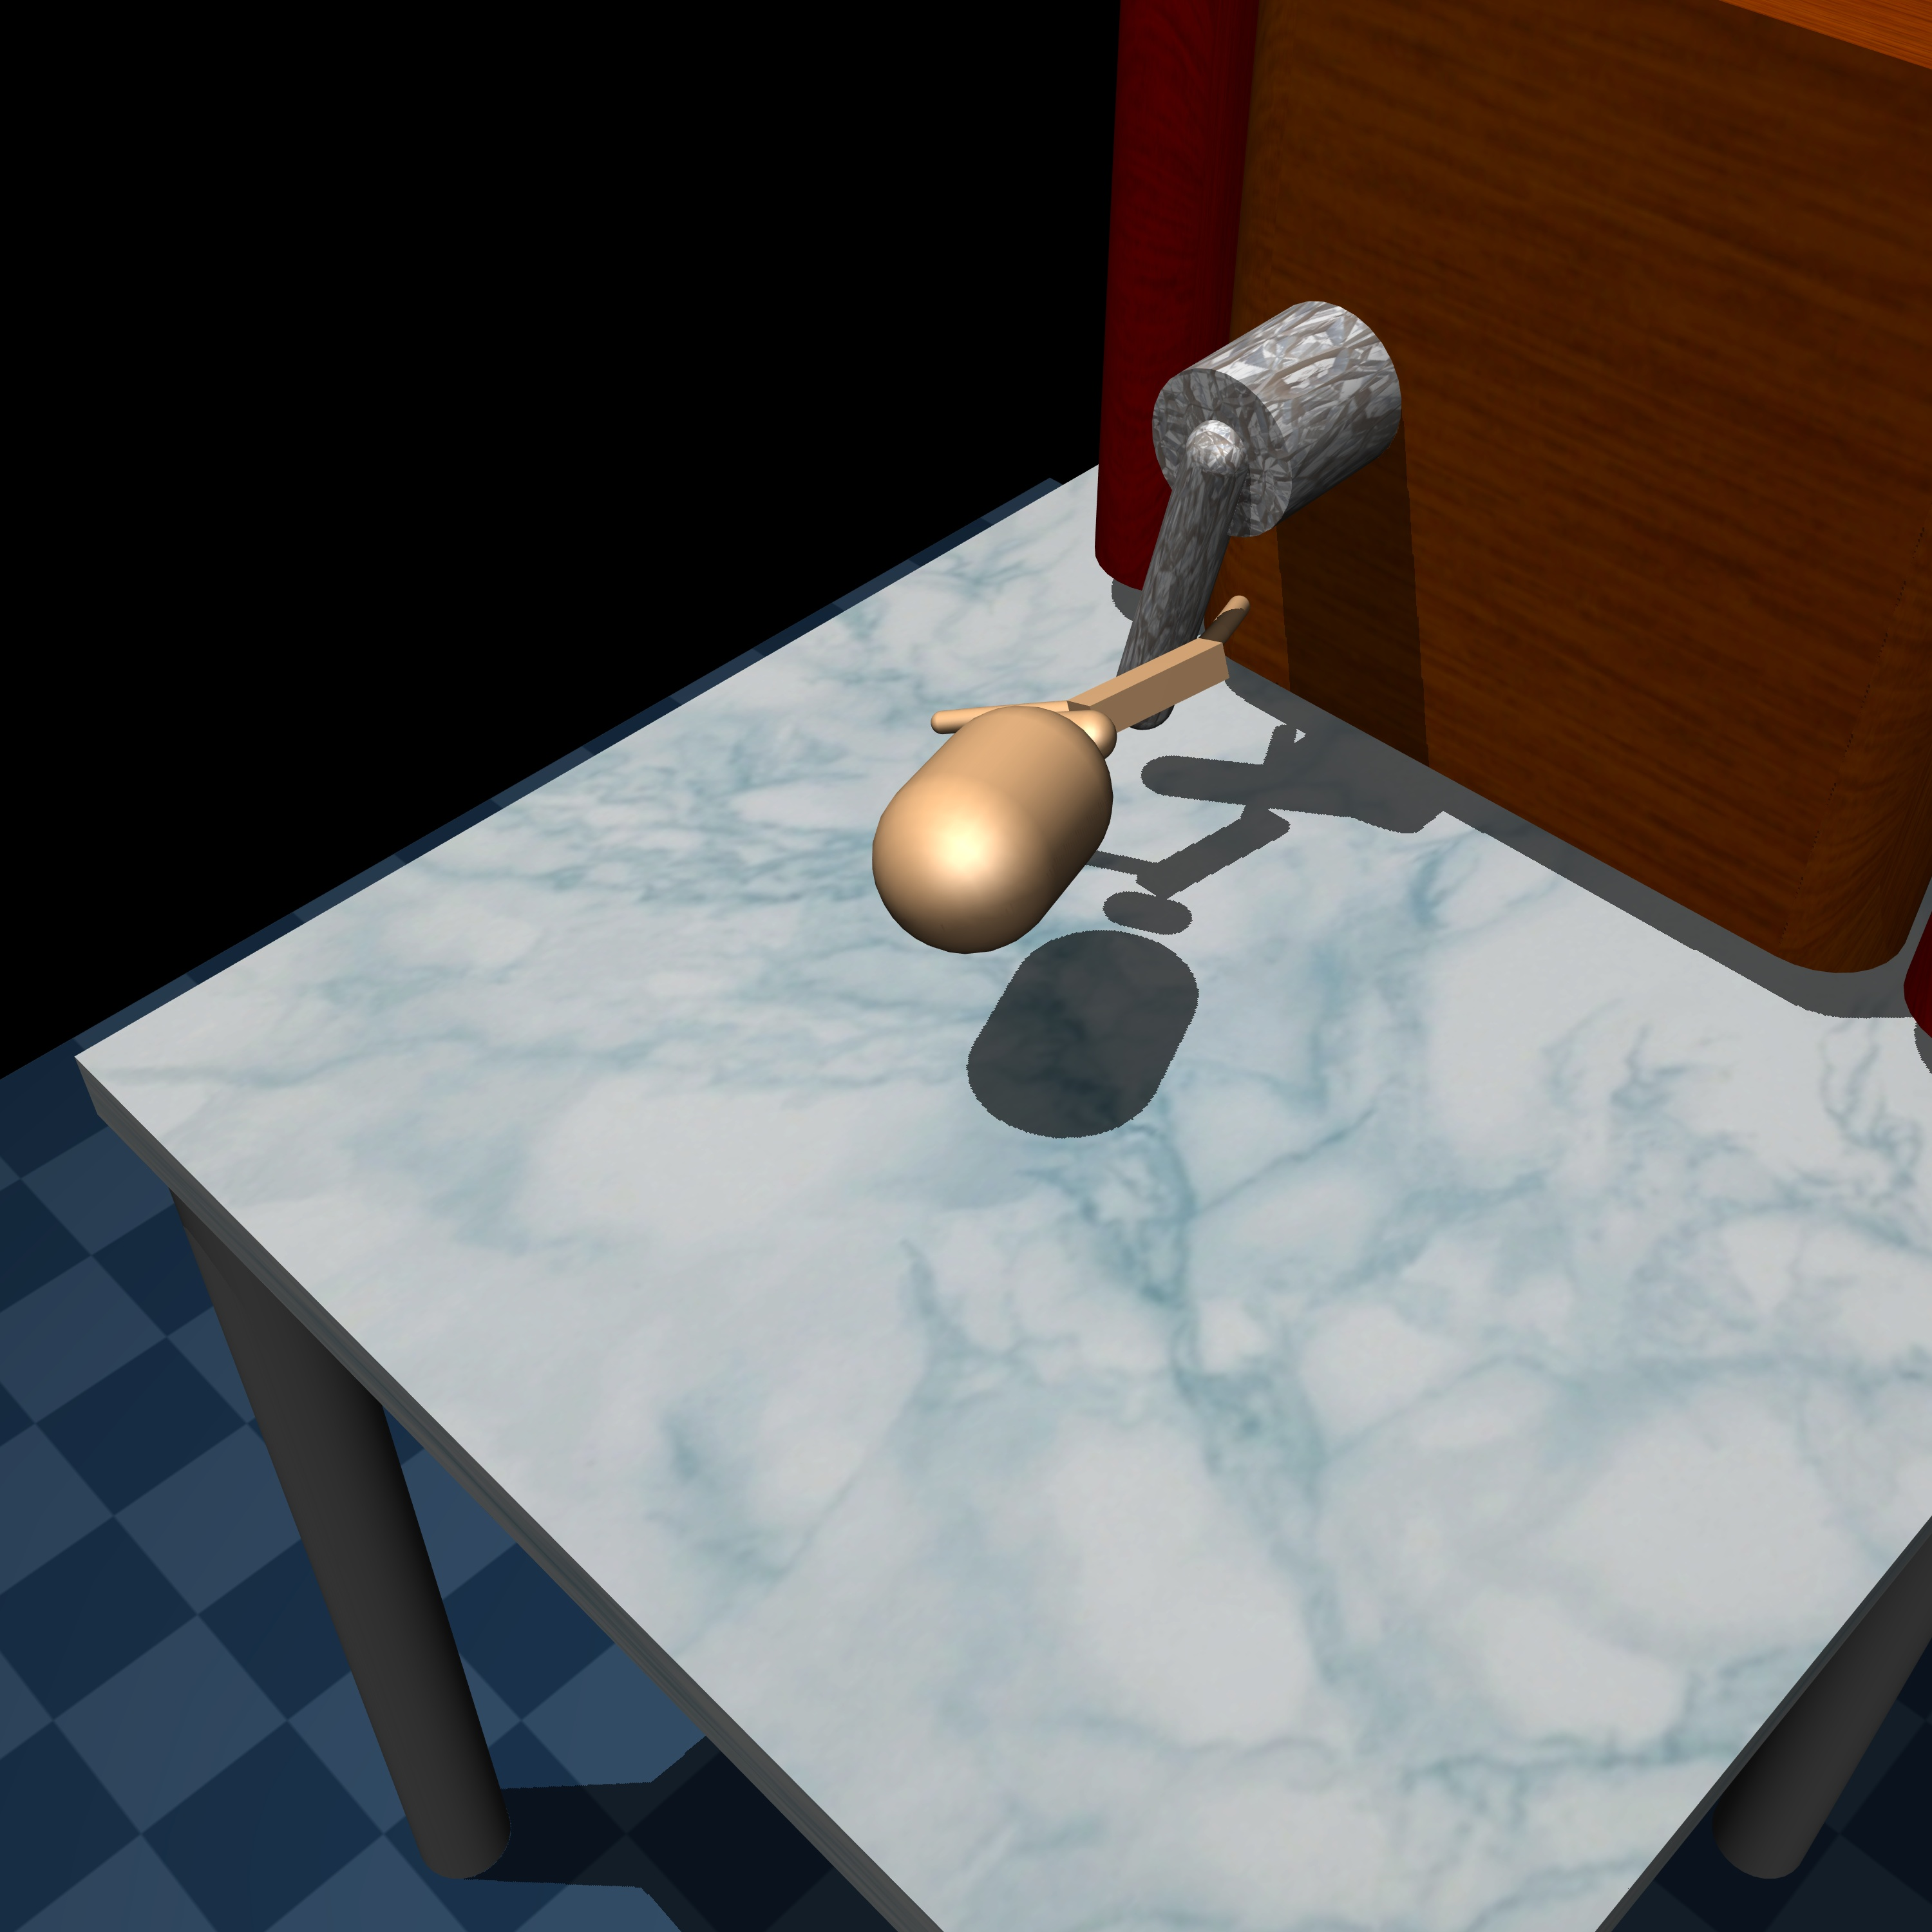
\includegraphics[width=\suppwidth\textwidth,valign=m]{Figures/supp/door/evolve/interp_1.0_image-0035.jpg} \\ \\
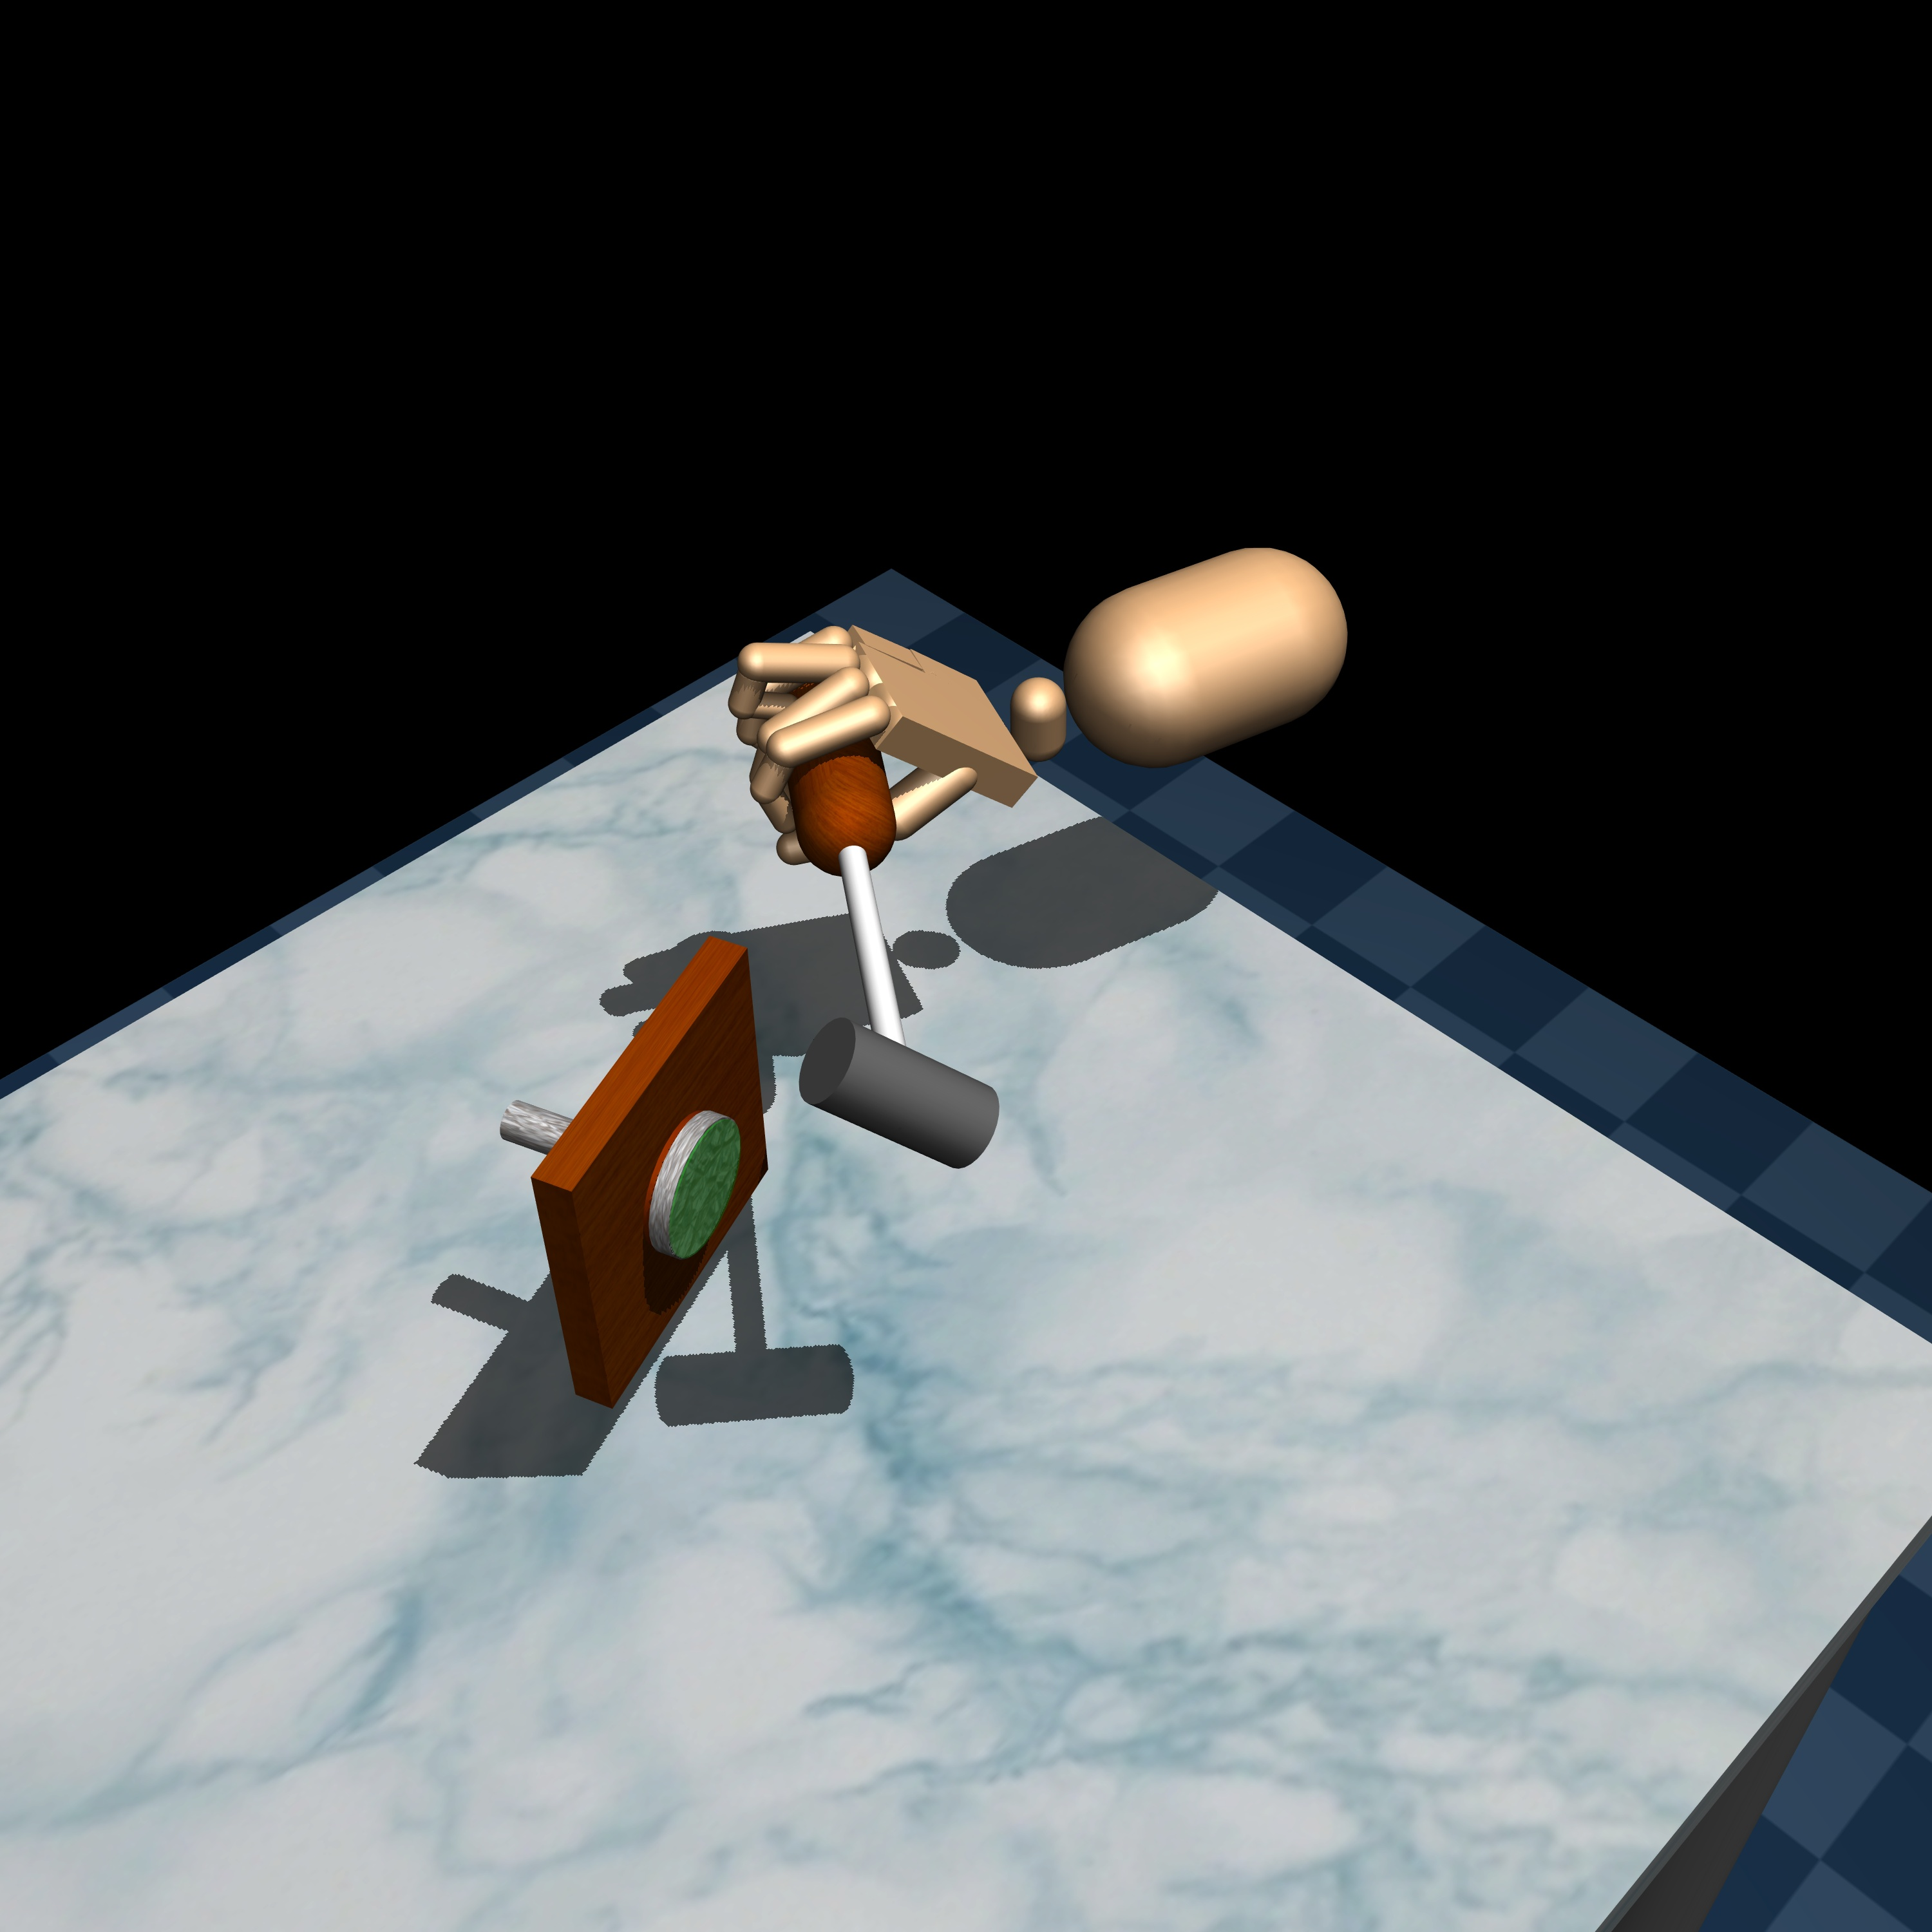
\includegraphics[width=\suppwidth\textwidth, valign=m]{Figures/supp/hammer/evolve/interp_0.0_image-0199.jpg}
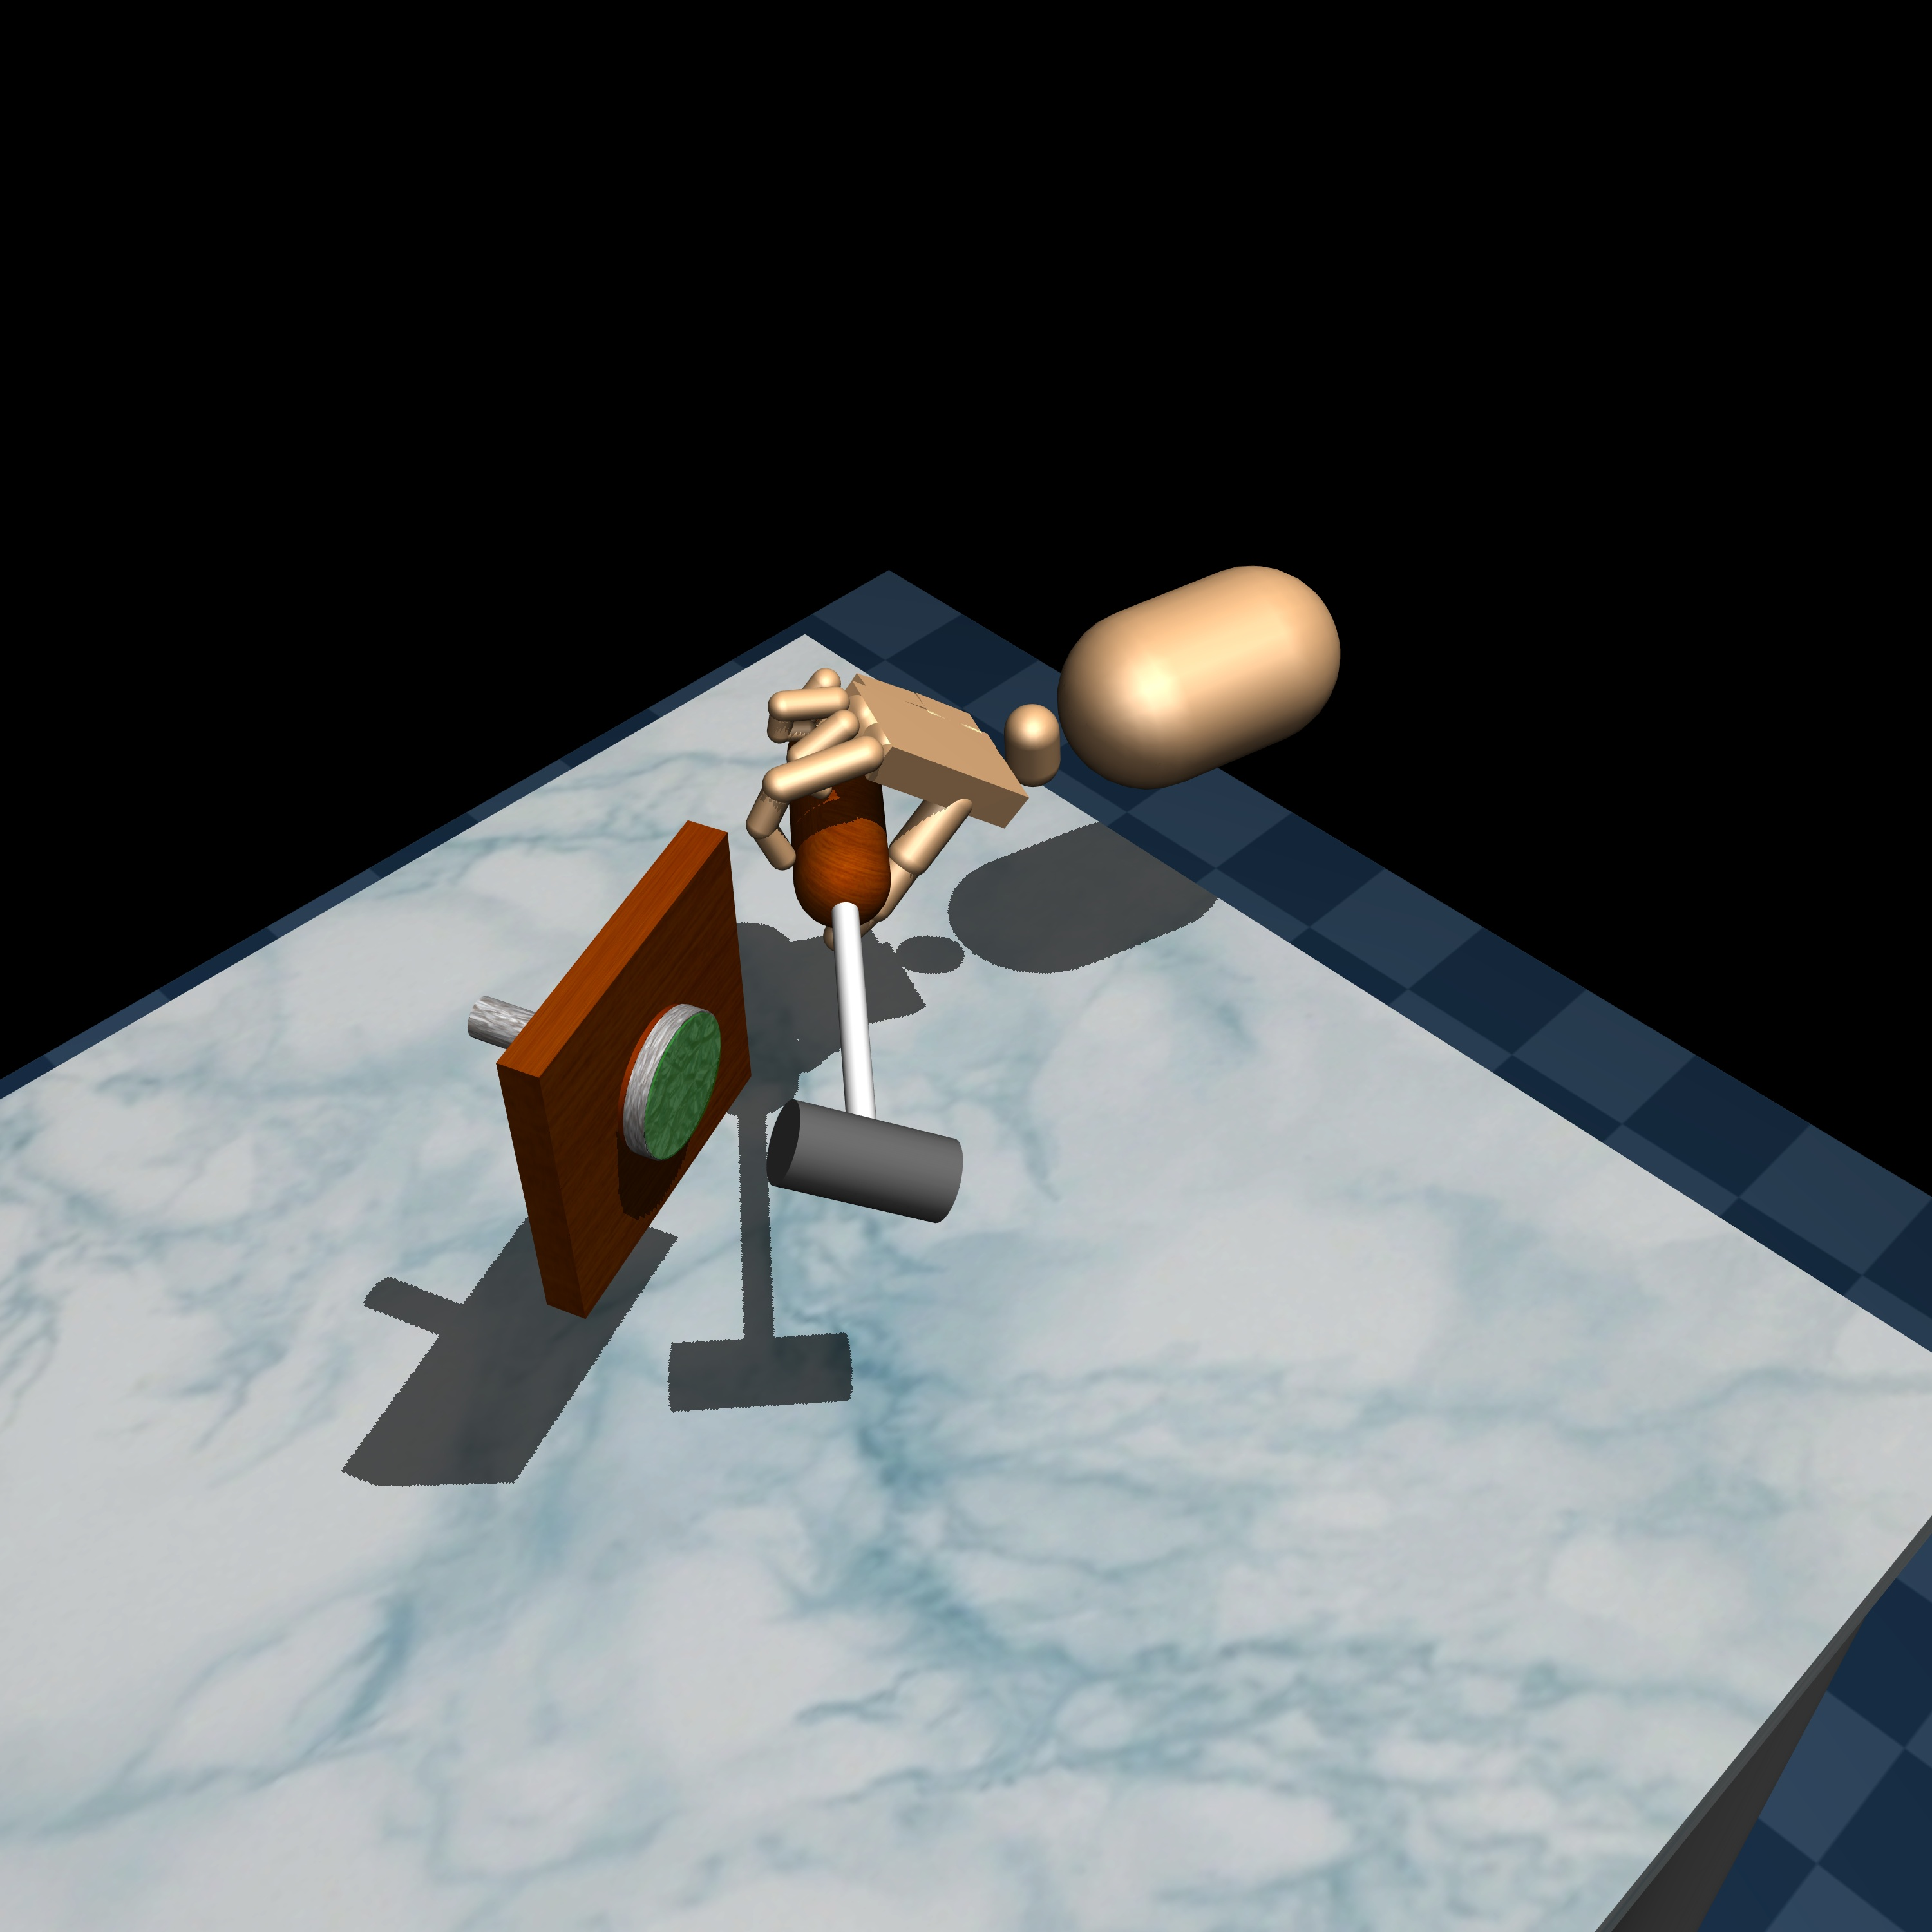
\includegraphics[width=\suppwidth\textwidth,valign=m]{Figures/supp/hammer/evolve/interp_0.2_image-0199.jpg}
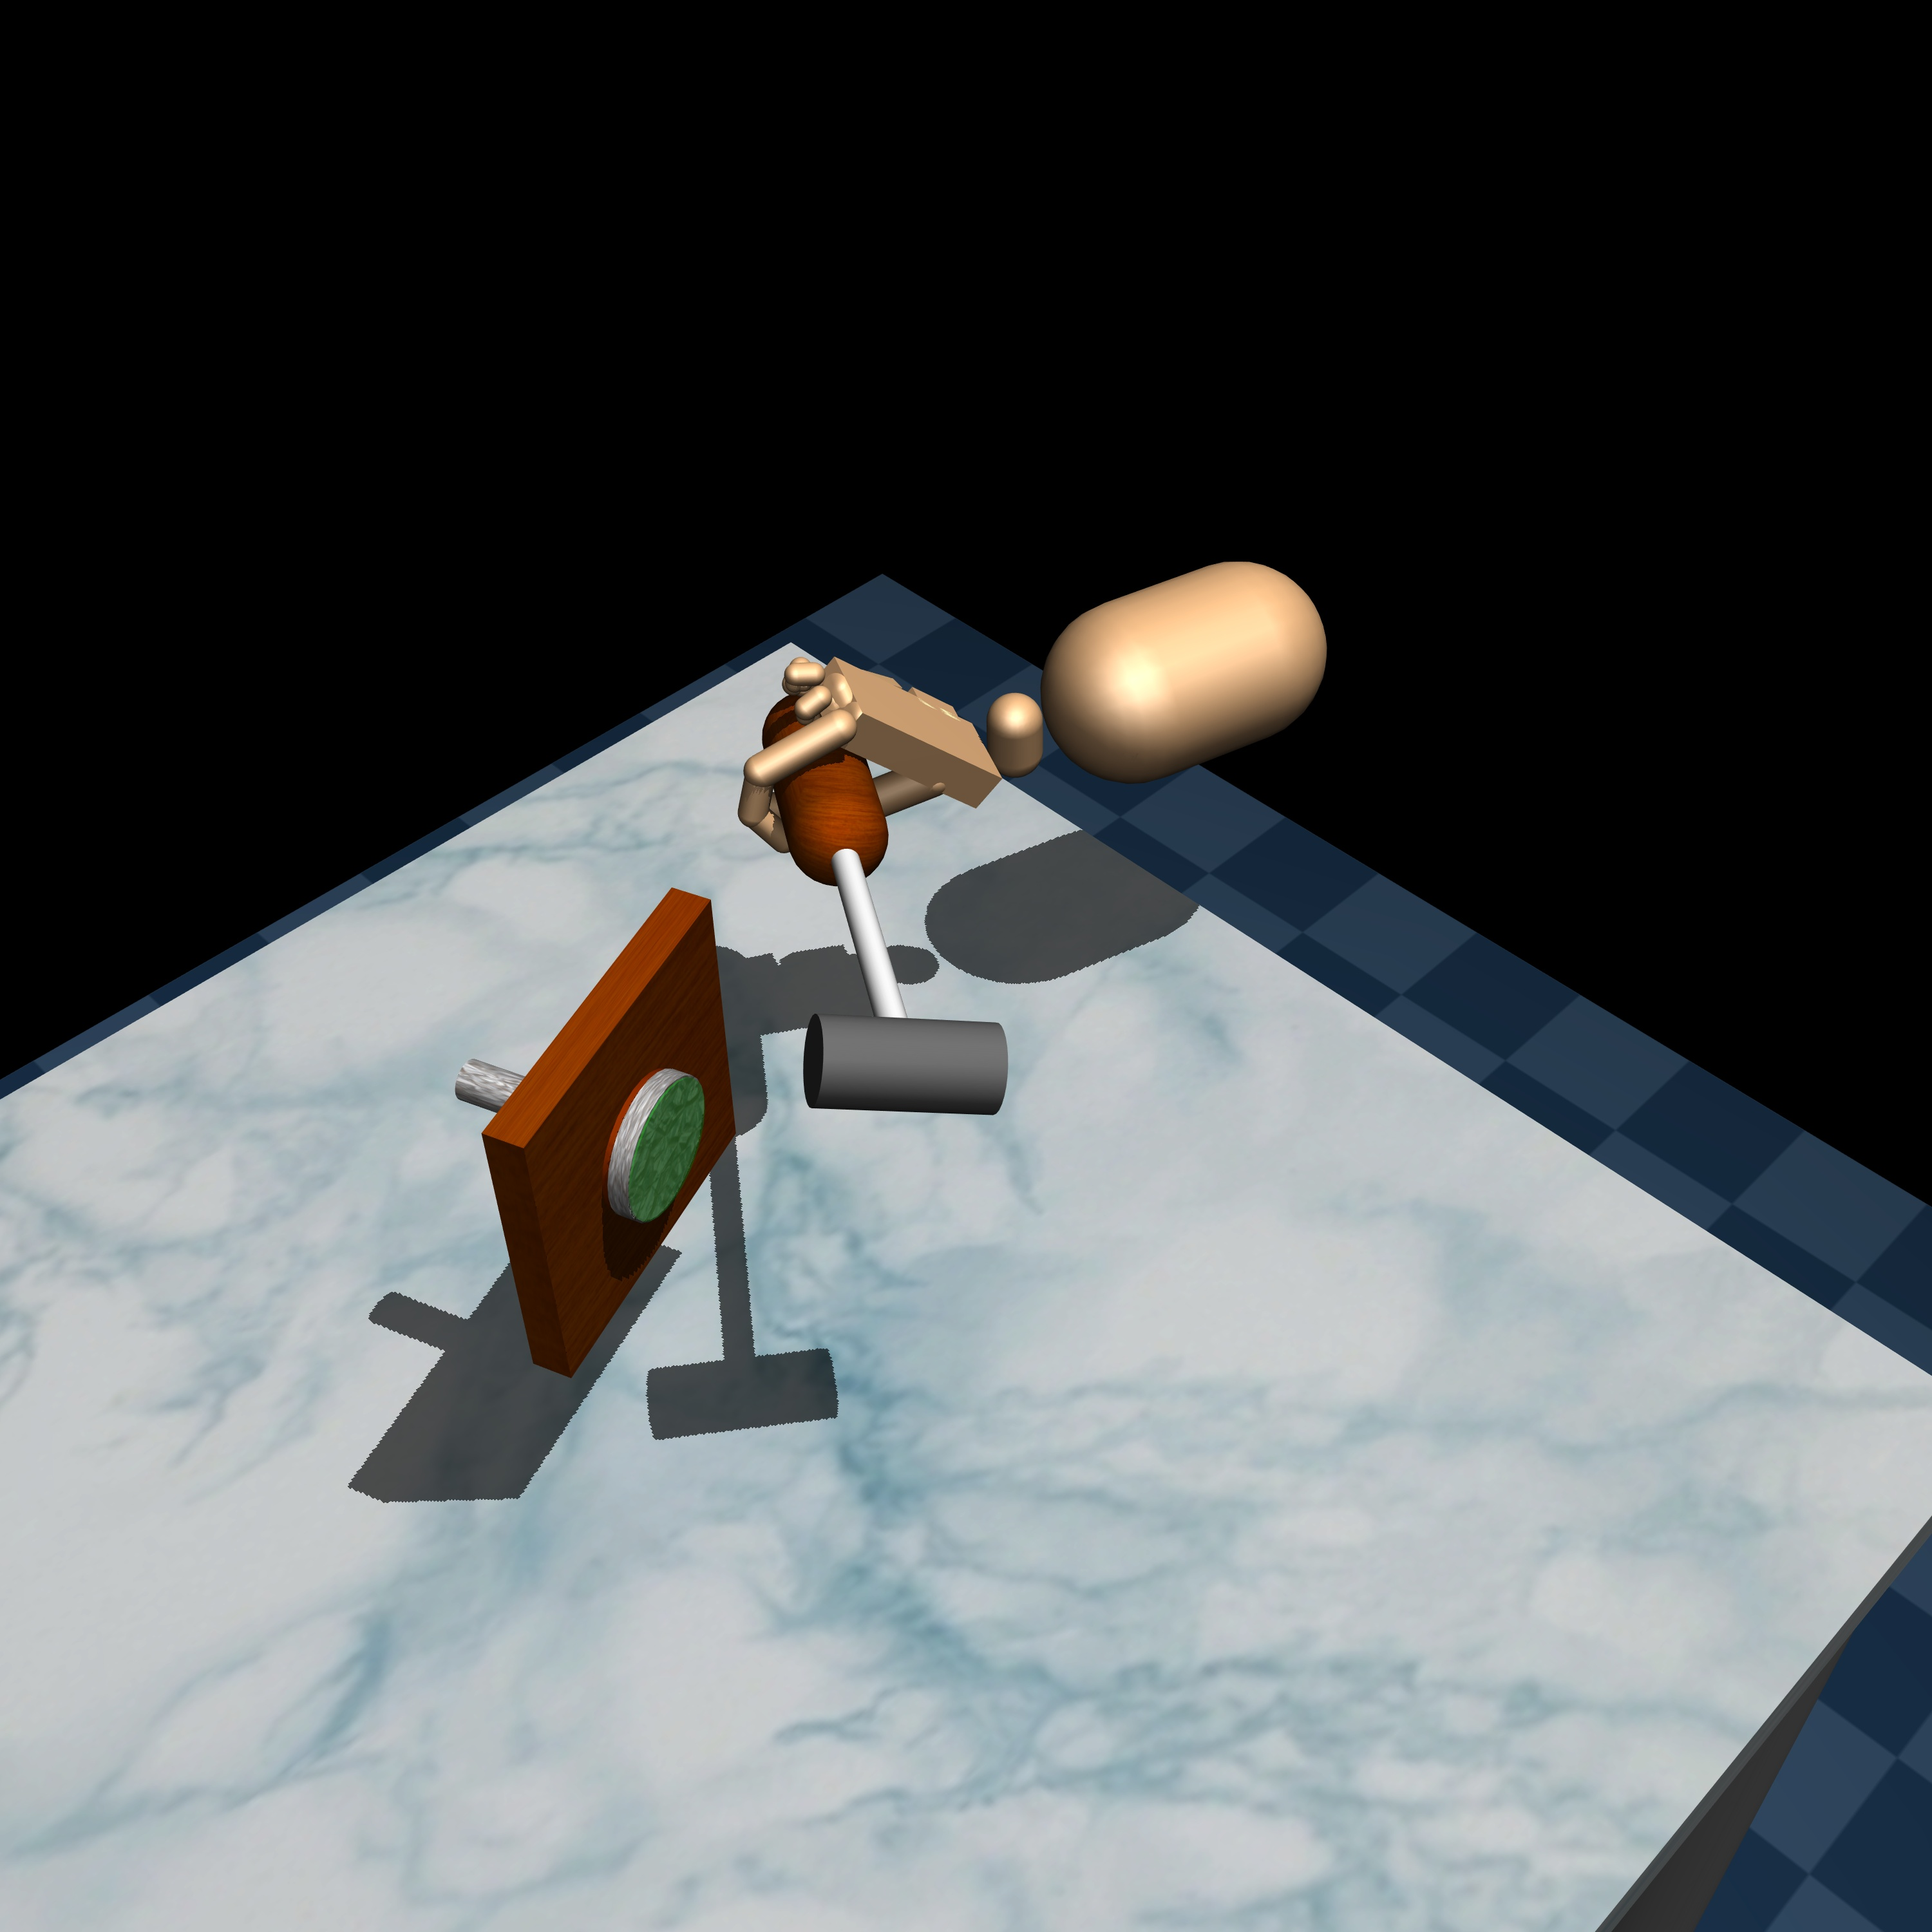
\includegraphics[width=\suppwidth\textwidth,valign=m]{Figures/supp/hammer/evolve/interp_0.4_image-0199.jpg}
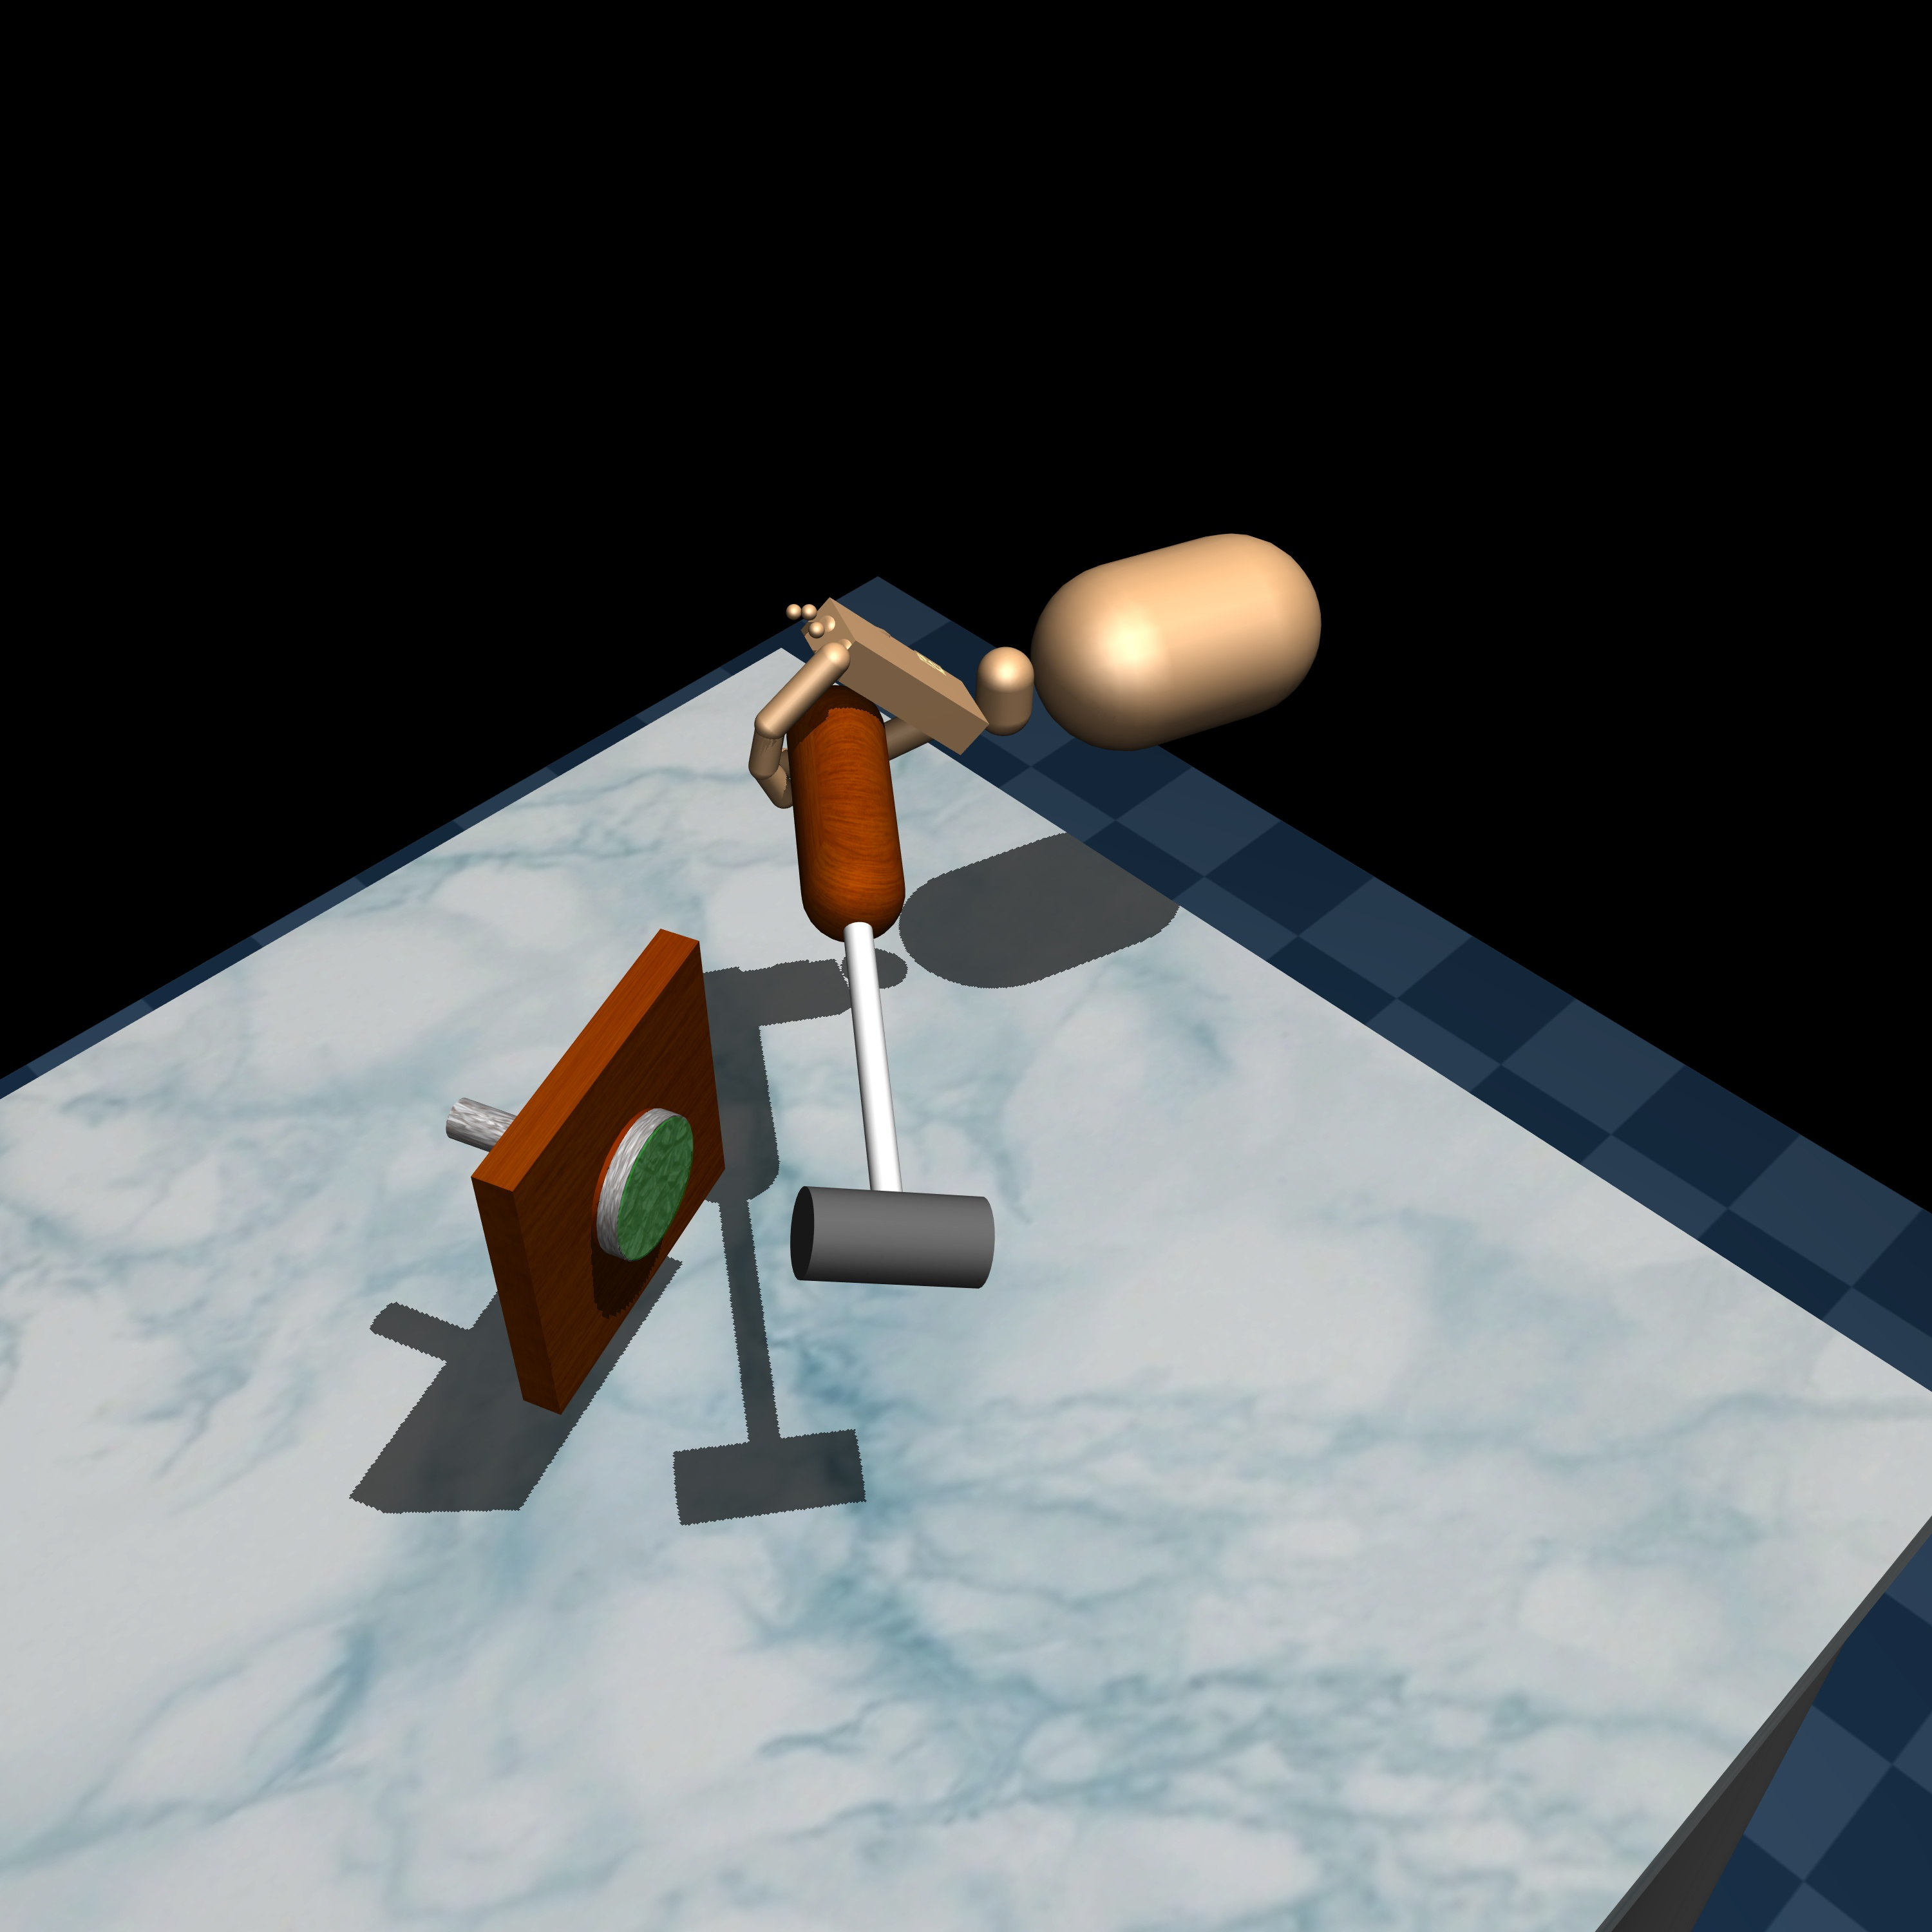
\includegraphics[width=\suppwidth\textwidth, valign=m]{Figures/supp/hammer/evolve/interp_0.6_image-0199.jpg}
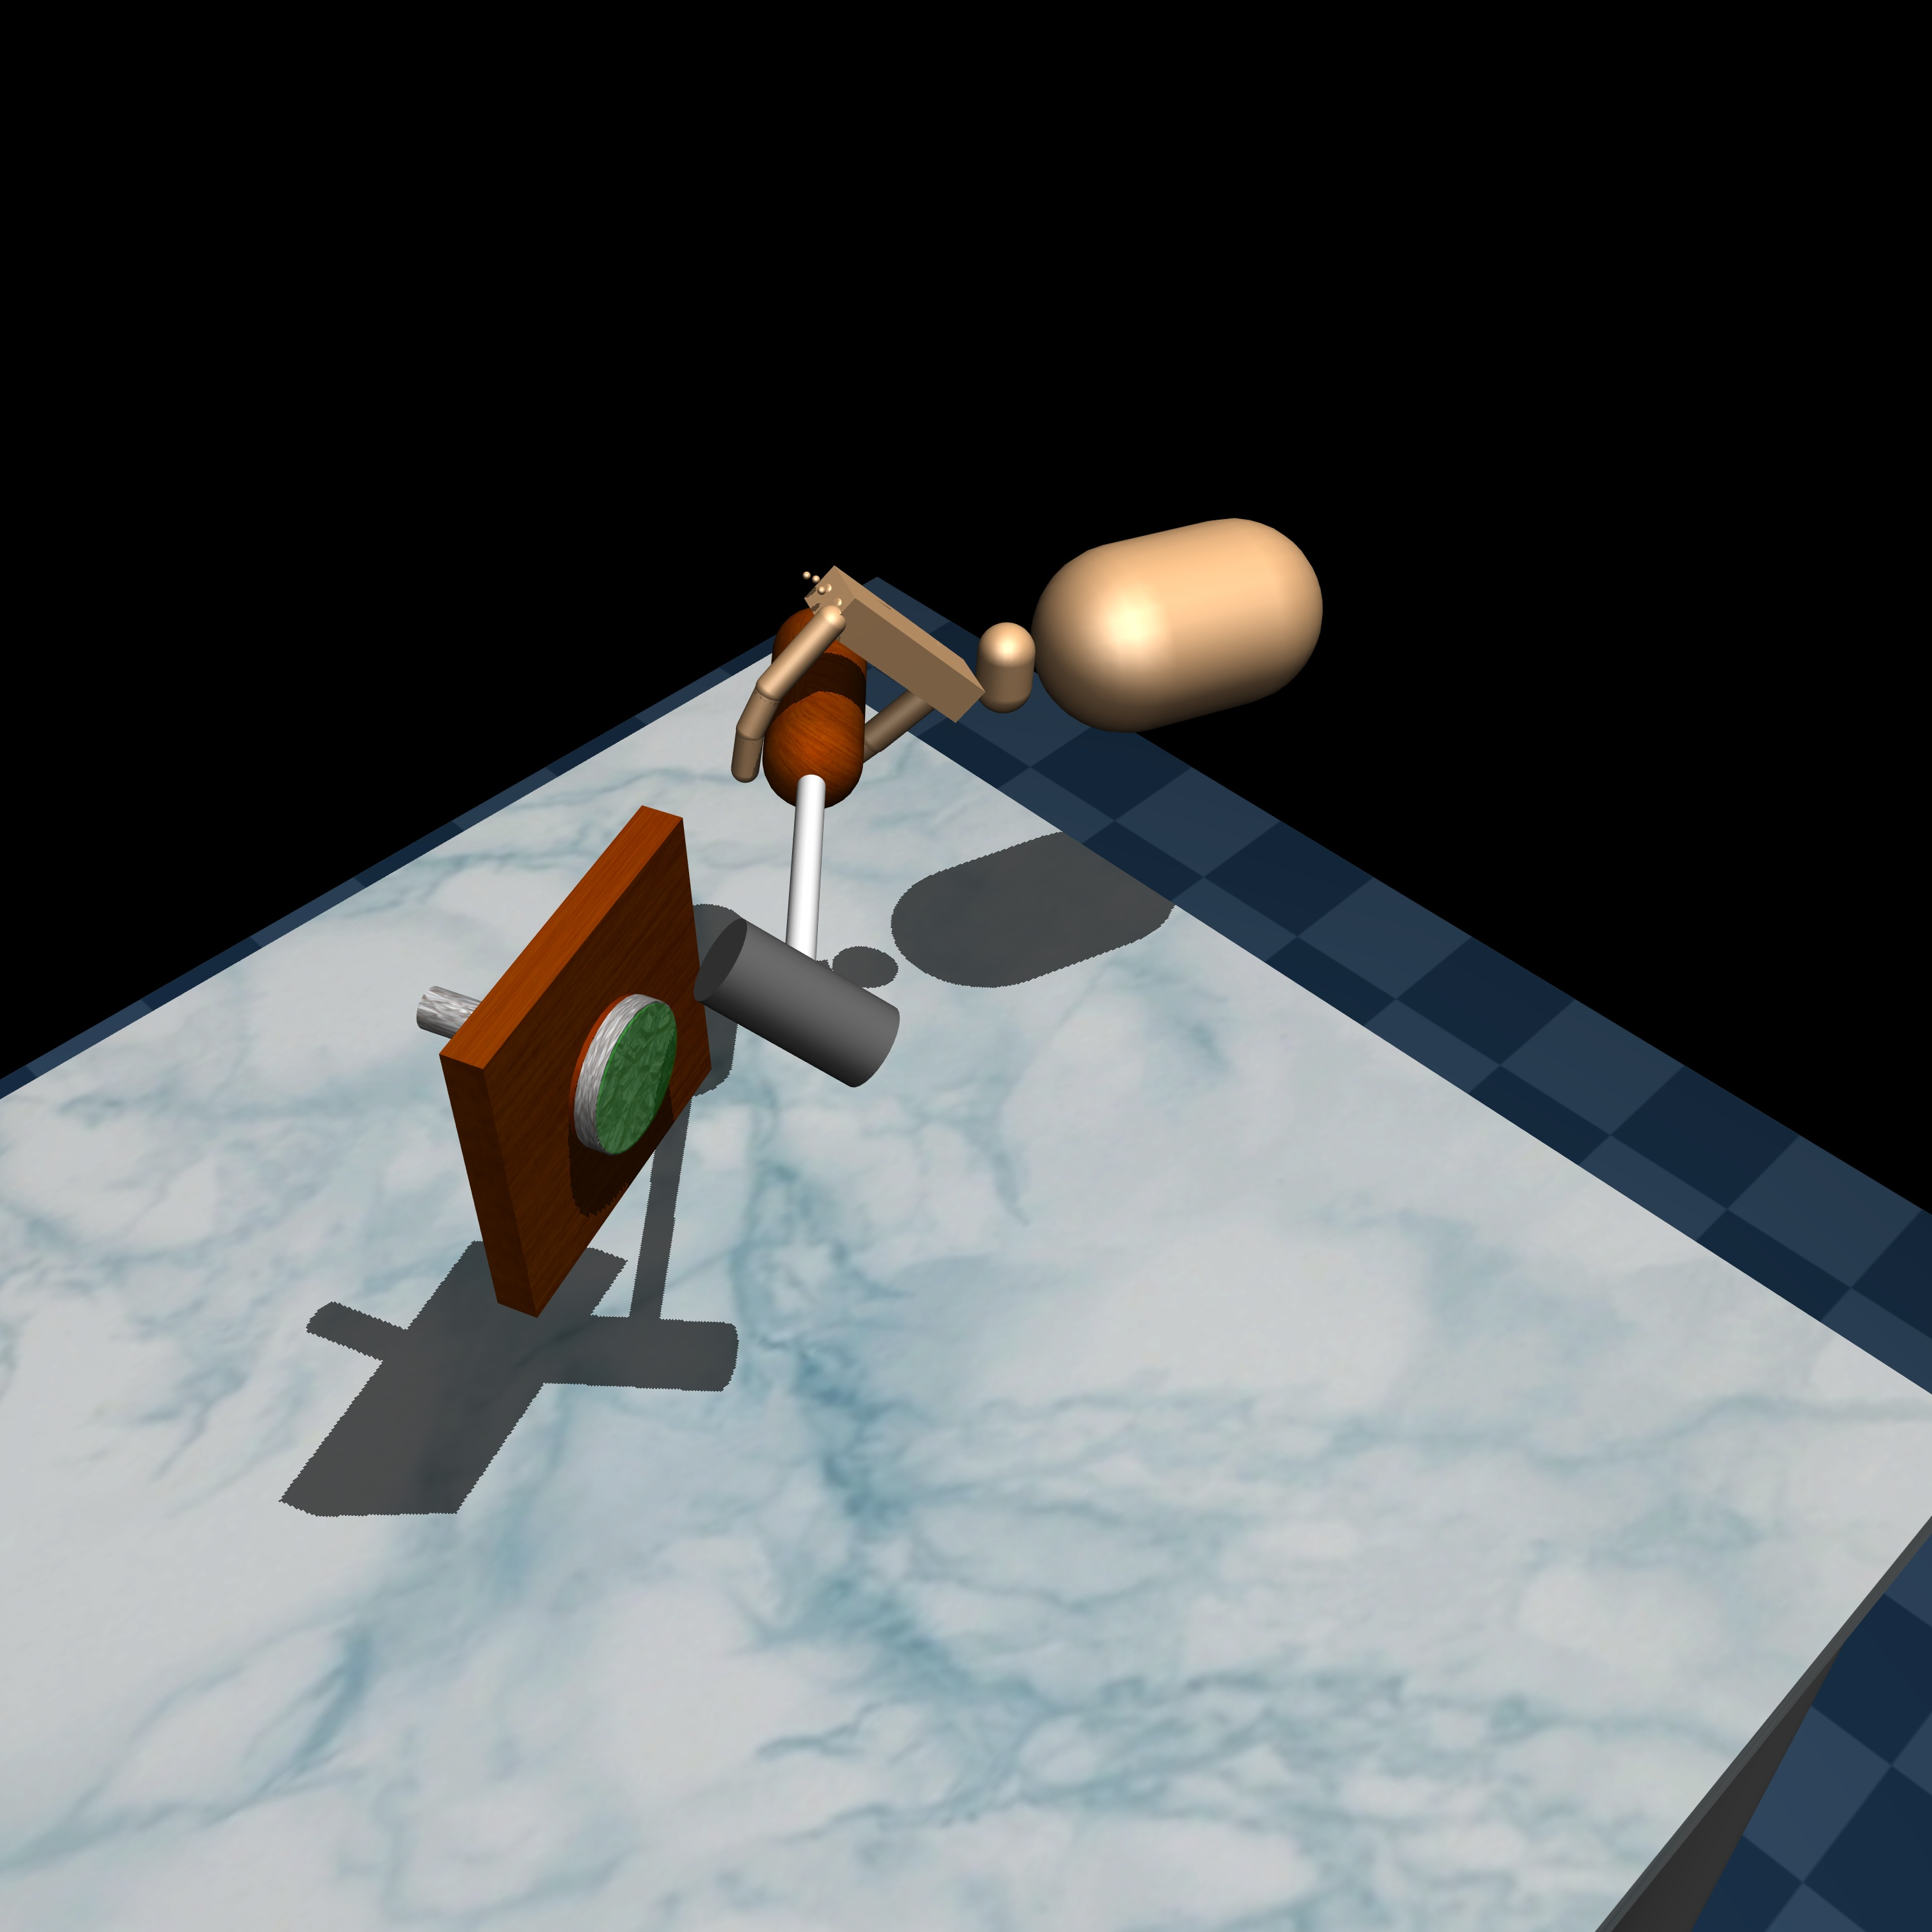
\includegraphics[width=\suppwidth\textwidth,valign=m]{Figures/supp/hammer/evolve/interp_0.8_image-0199.jpg}
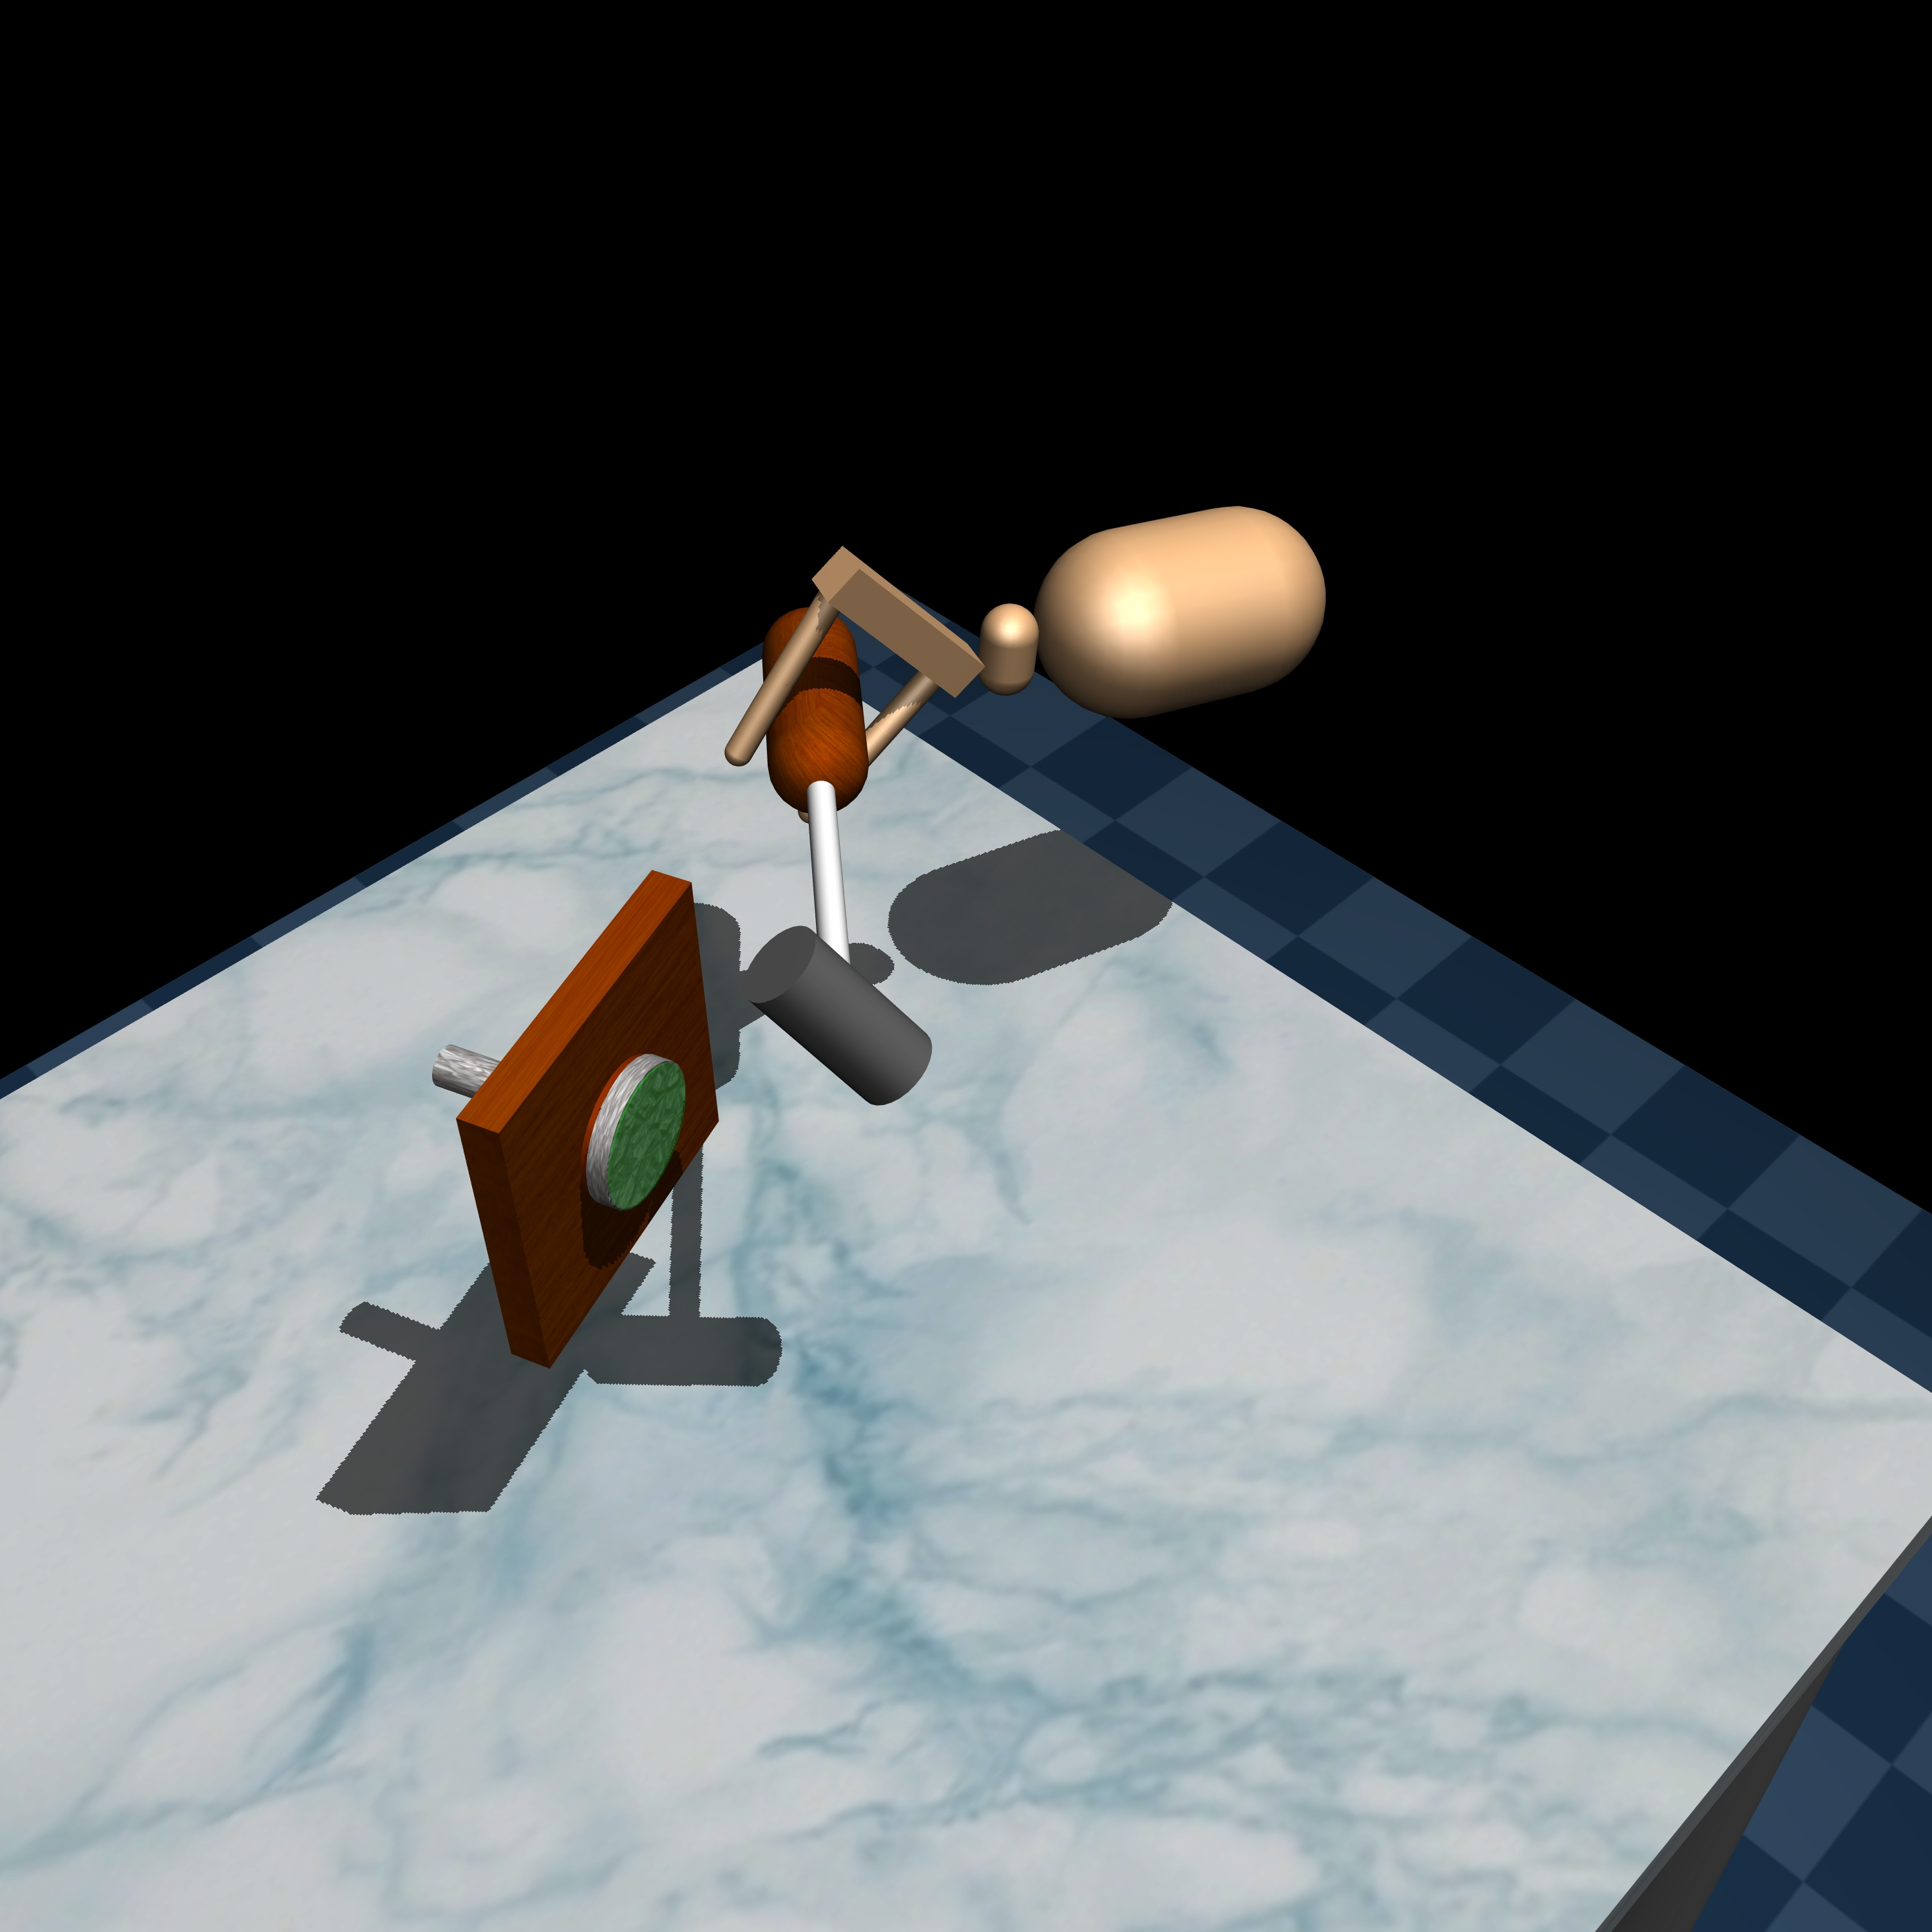
\includegraphics[width=\suppwidth\textwidth,valign=m]{Figures/supp/hammer/evolve/interp_1.0_image-0199.jpg} \\ \\

\includegraphics[width=\suppwidth\textwidth,valign=m]{Figures/supp/relocate/evolve/interp_0.0_image-0199.jpg}

\includegraphics[width=\suppwidth\textwidth,valign=m]{Figures/supp/relocate/evolve/interp_0.2_image-0199.jpg}

\includegraphics[width=\suppwidth\textwidth,valign=m]{Figures/supp/relocate/evolve/interp_0.4_image-0199.jpg}

\includegraphics[width=\suppwidth\textwidth,valign=m]{Figures/supp/relocate/evolve/interp_0.6_image-0199.jpg}

\includegraphics[width=\suppwidth\textwidth,valign=m]{Figures/supp/relocate/evolve/interp_0.8_image-0199.jpg}

\includegraphics[width=\suppwidth\textwidth,valign=m]{Figures/supp/relocate/evolve/interp_1.0_image-0199.jpg}
\end{tabular}
\vspace{-1ex}
\caption{
\textbf{Visualization of policy on evolving intermediate robots on Hand Manipulation Suite tasks.}
The three rows shows  \texttt{Door}, \texttt{Hammer}, and \texttt{Relocate} tasks respectively.
From left to right in each row, we show a snapshot of robot at evolution parameters $\alpha$ at $0, 0.2, 0.4, 0.6, 0.8, 1$ respectively in the six columns.
} 
\label{fig:dapg:evolve:viz}
\end{figure}


\begin{figure}[ht]
\centering
\newcommand\suppwidth{0.15}
\begin{tabular}{cccccc}
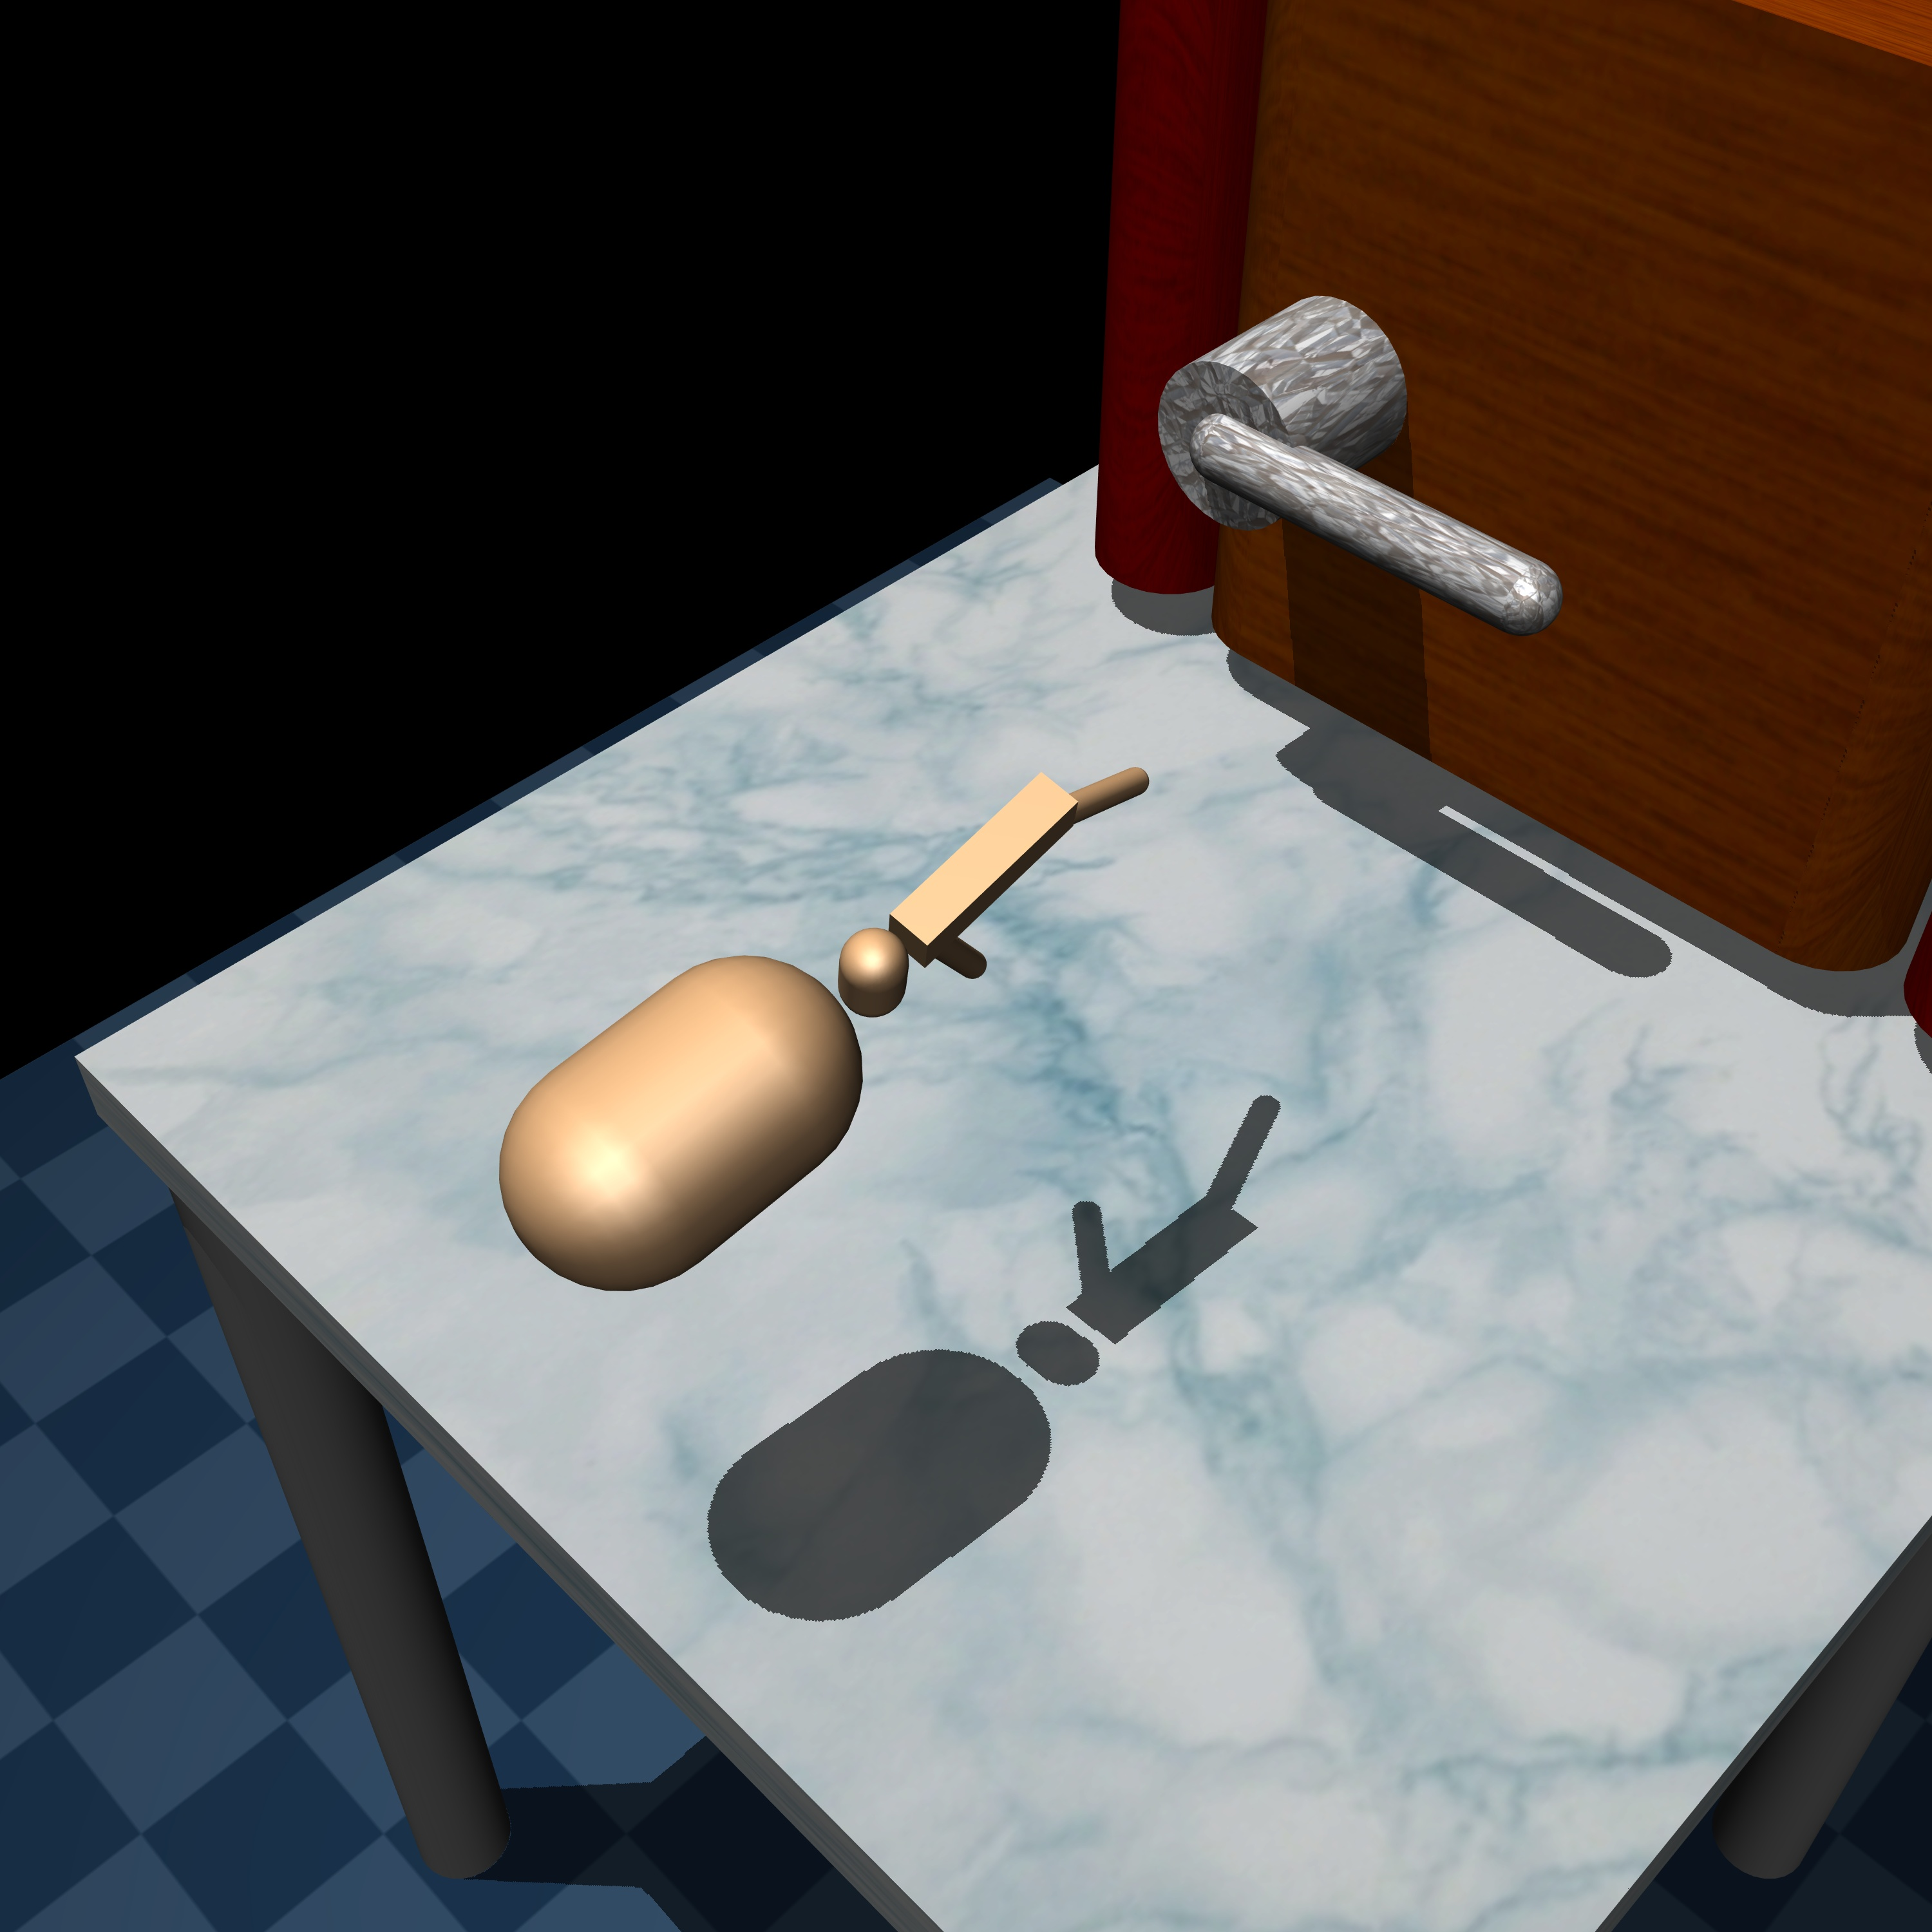
\includegraphics[width=\suppwidth\textwidth,valign=m]{Figures/supp/door/target/image-0005.jpg}
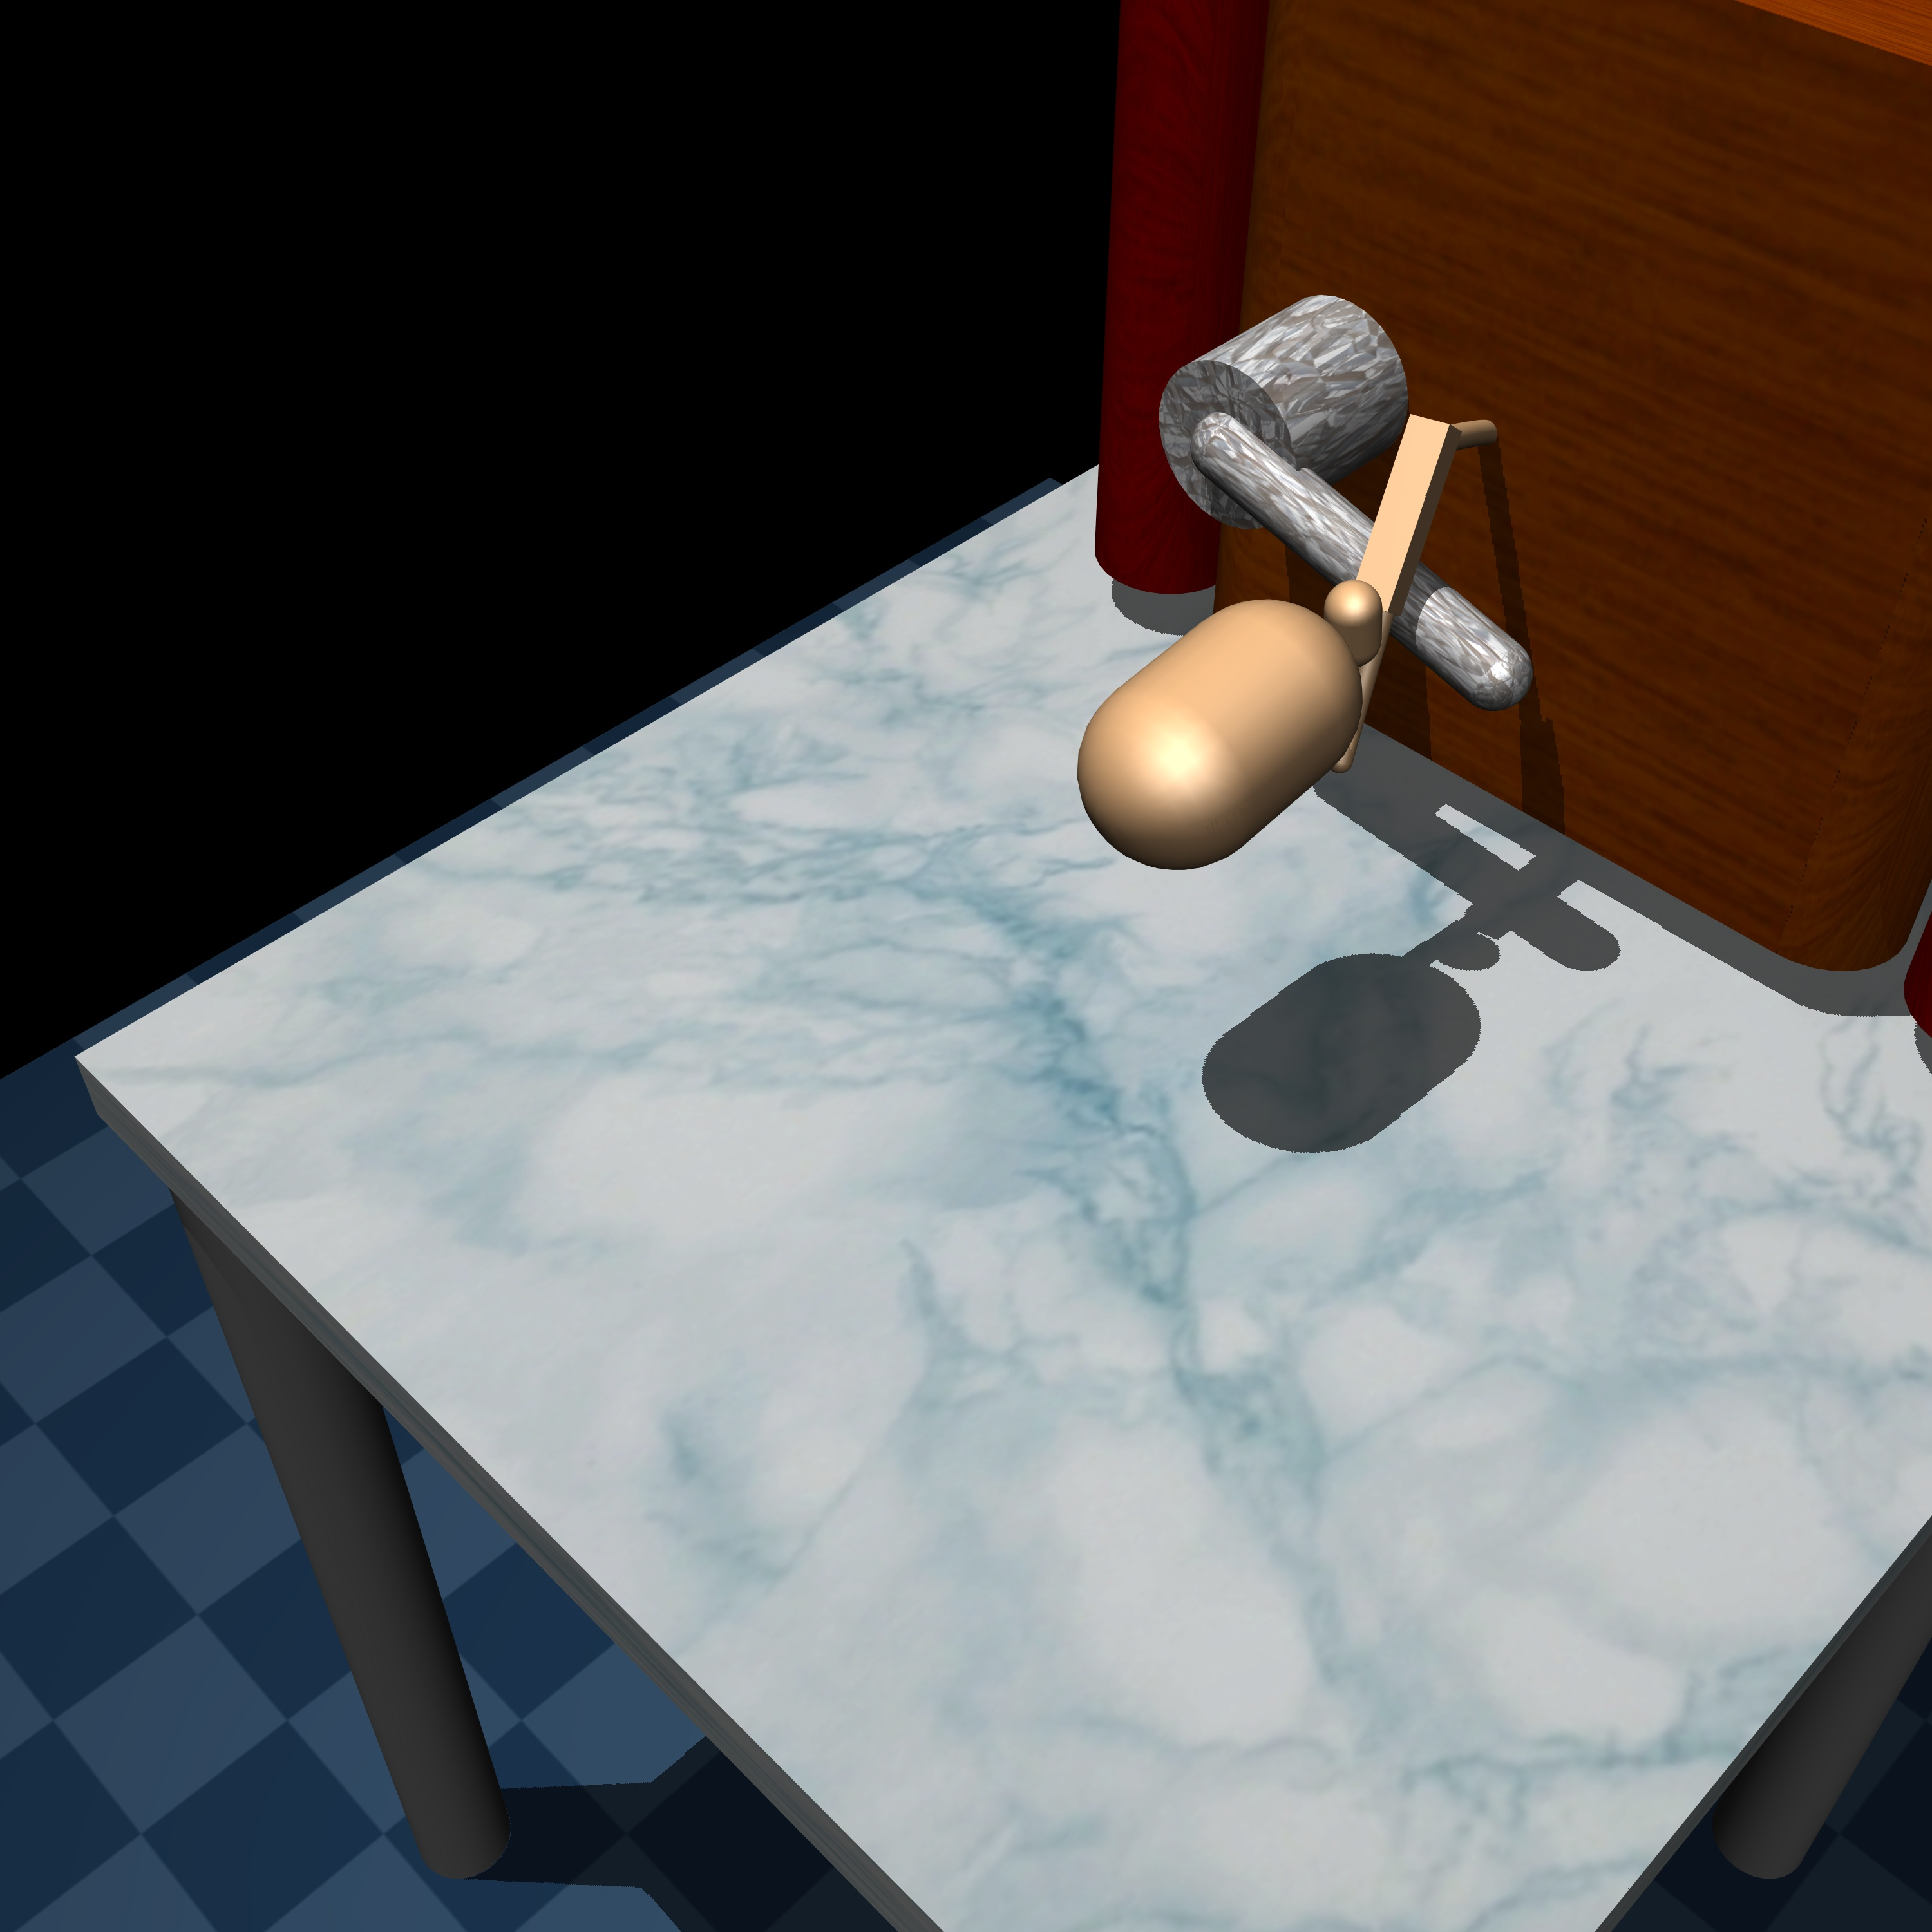
\includegraphics[width=\suppwidth\textwidth,valign=m]{Figures/supp/door/target/image-0020.jpg}
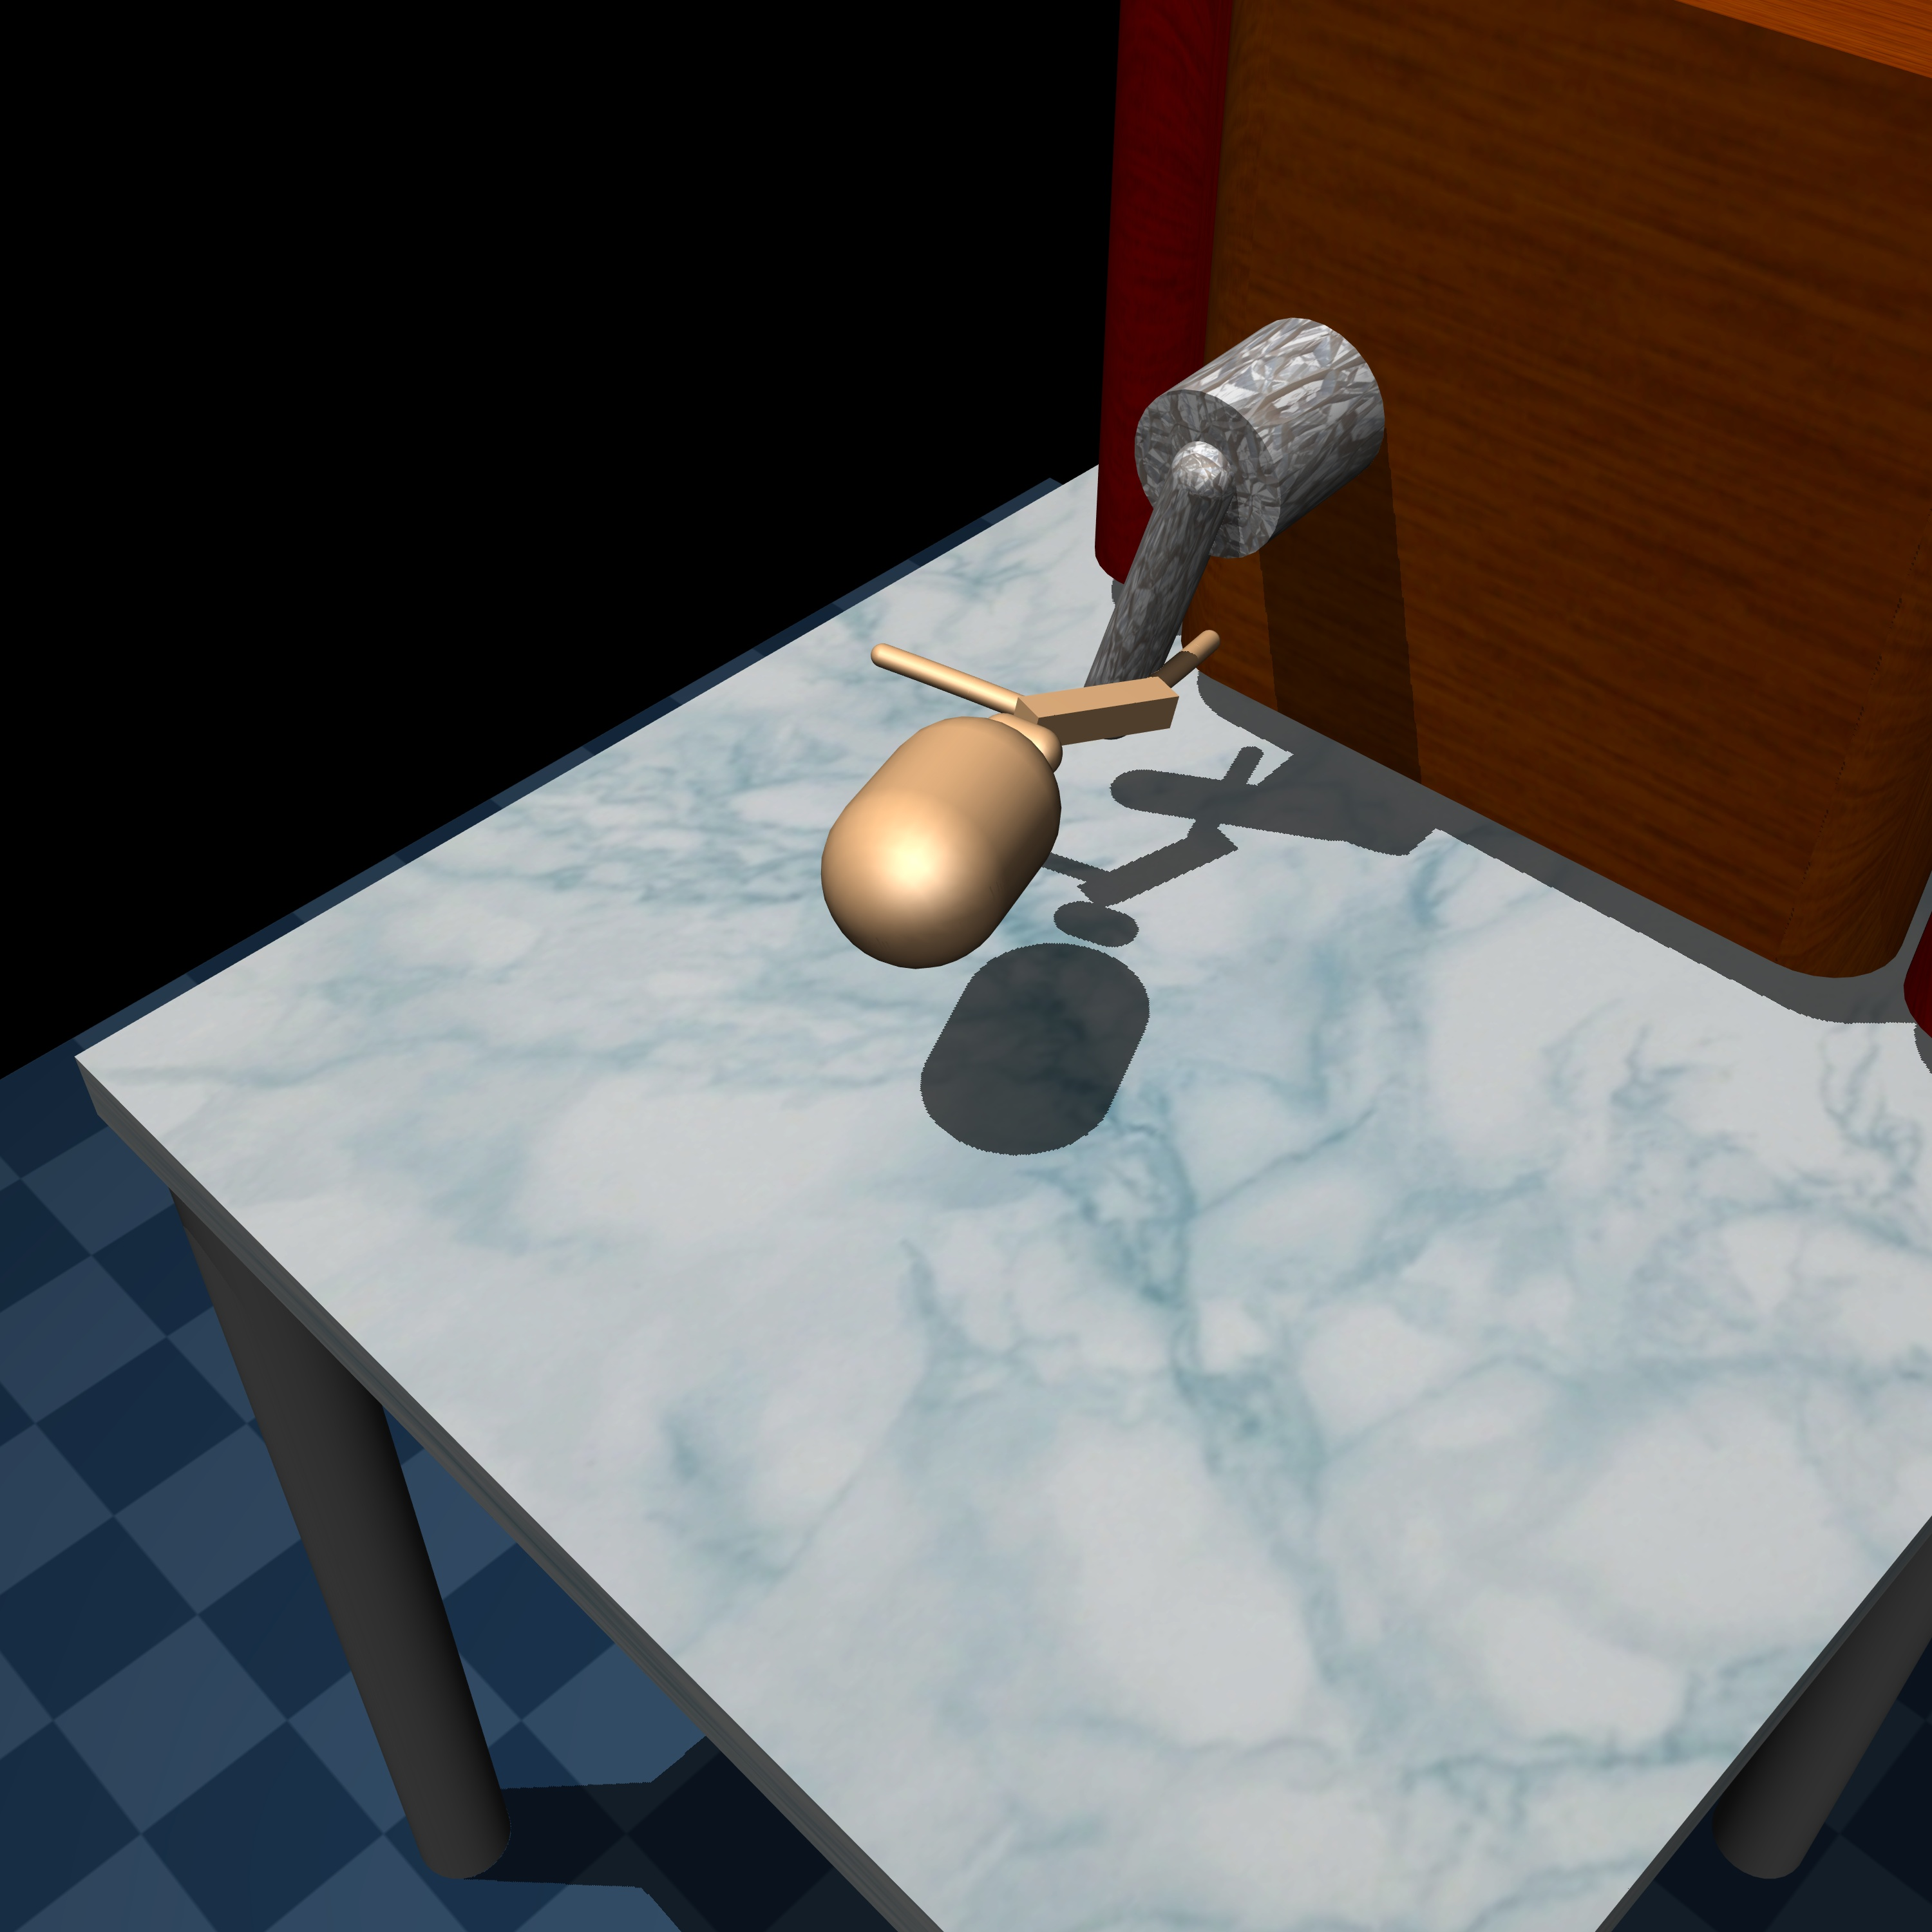
\includegraphics[width=\suppwidth\textwidth,valign=m]{Figures/supp/door/target/image-0040.jpg}
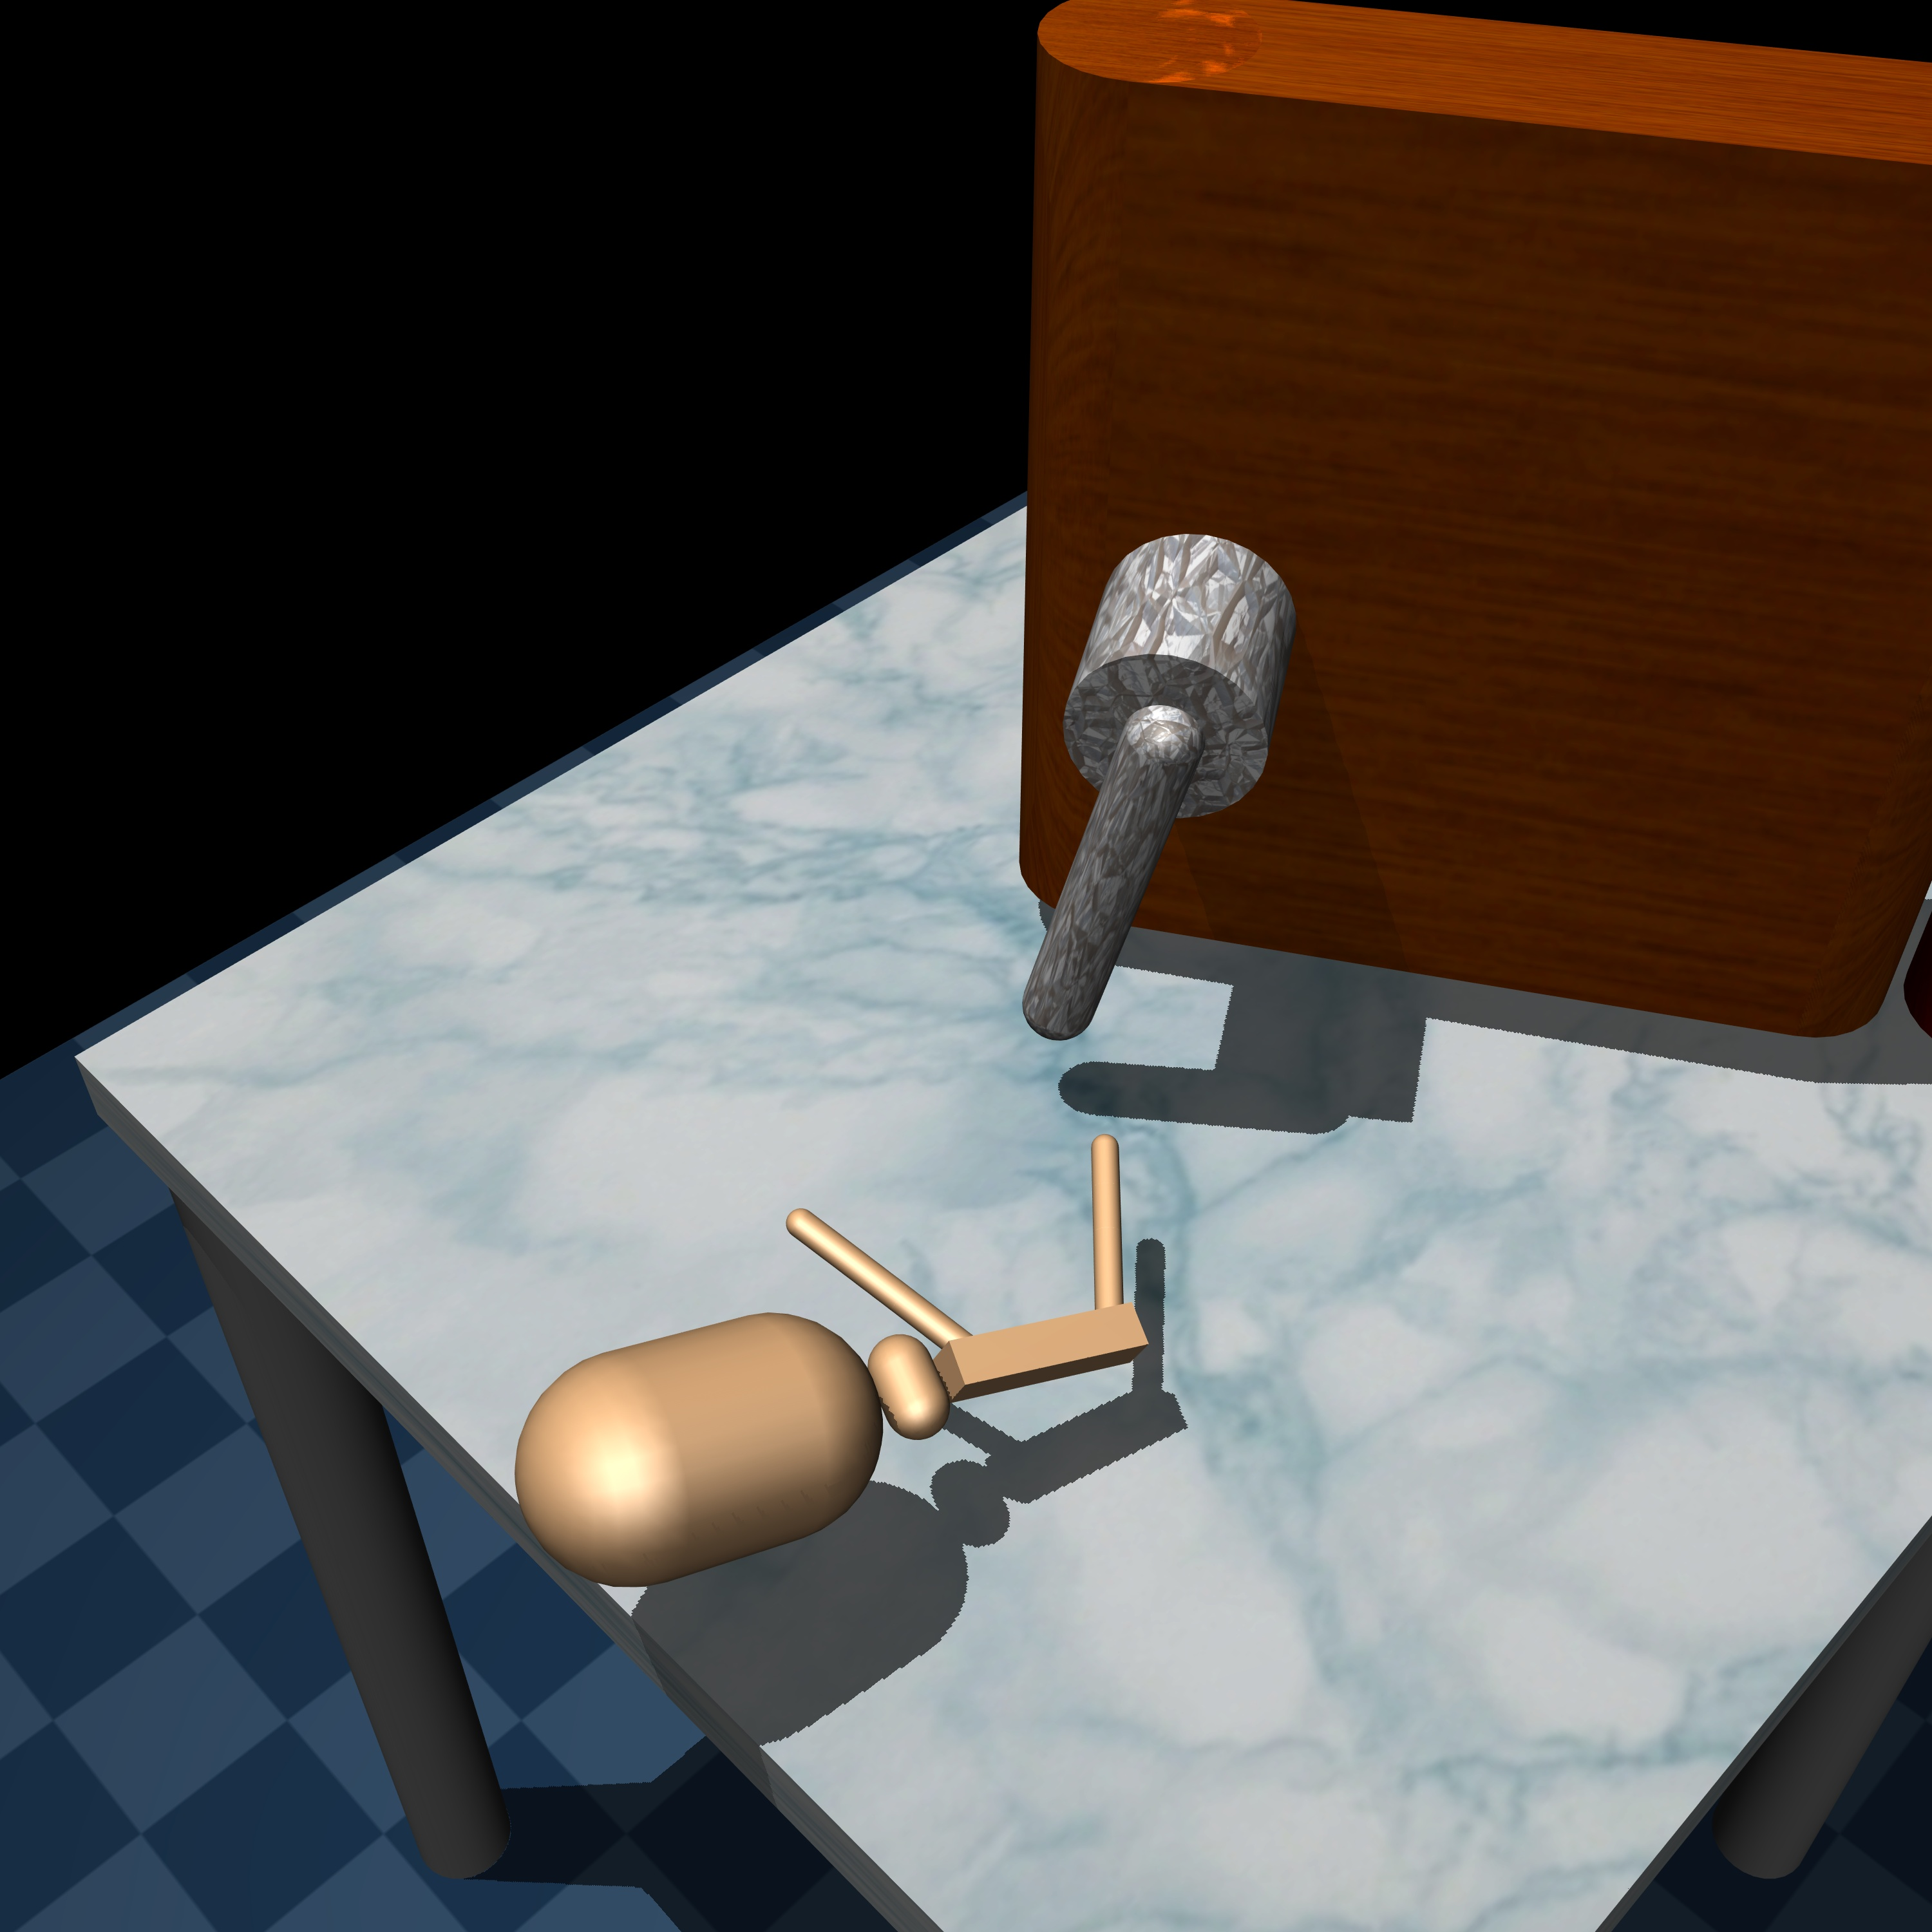
\includegraphics[width=\suppwidth\textwidth,valign=m]{Figures/supp/door/target/image-0060.jpg}
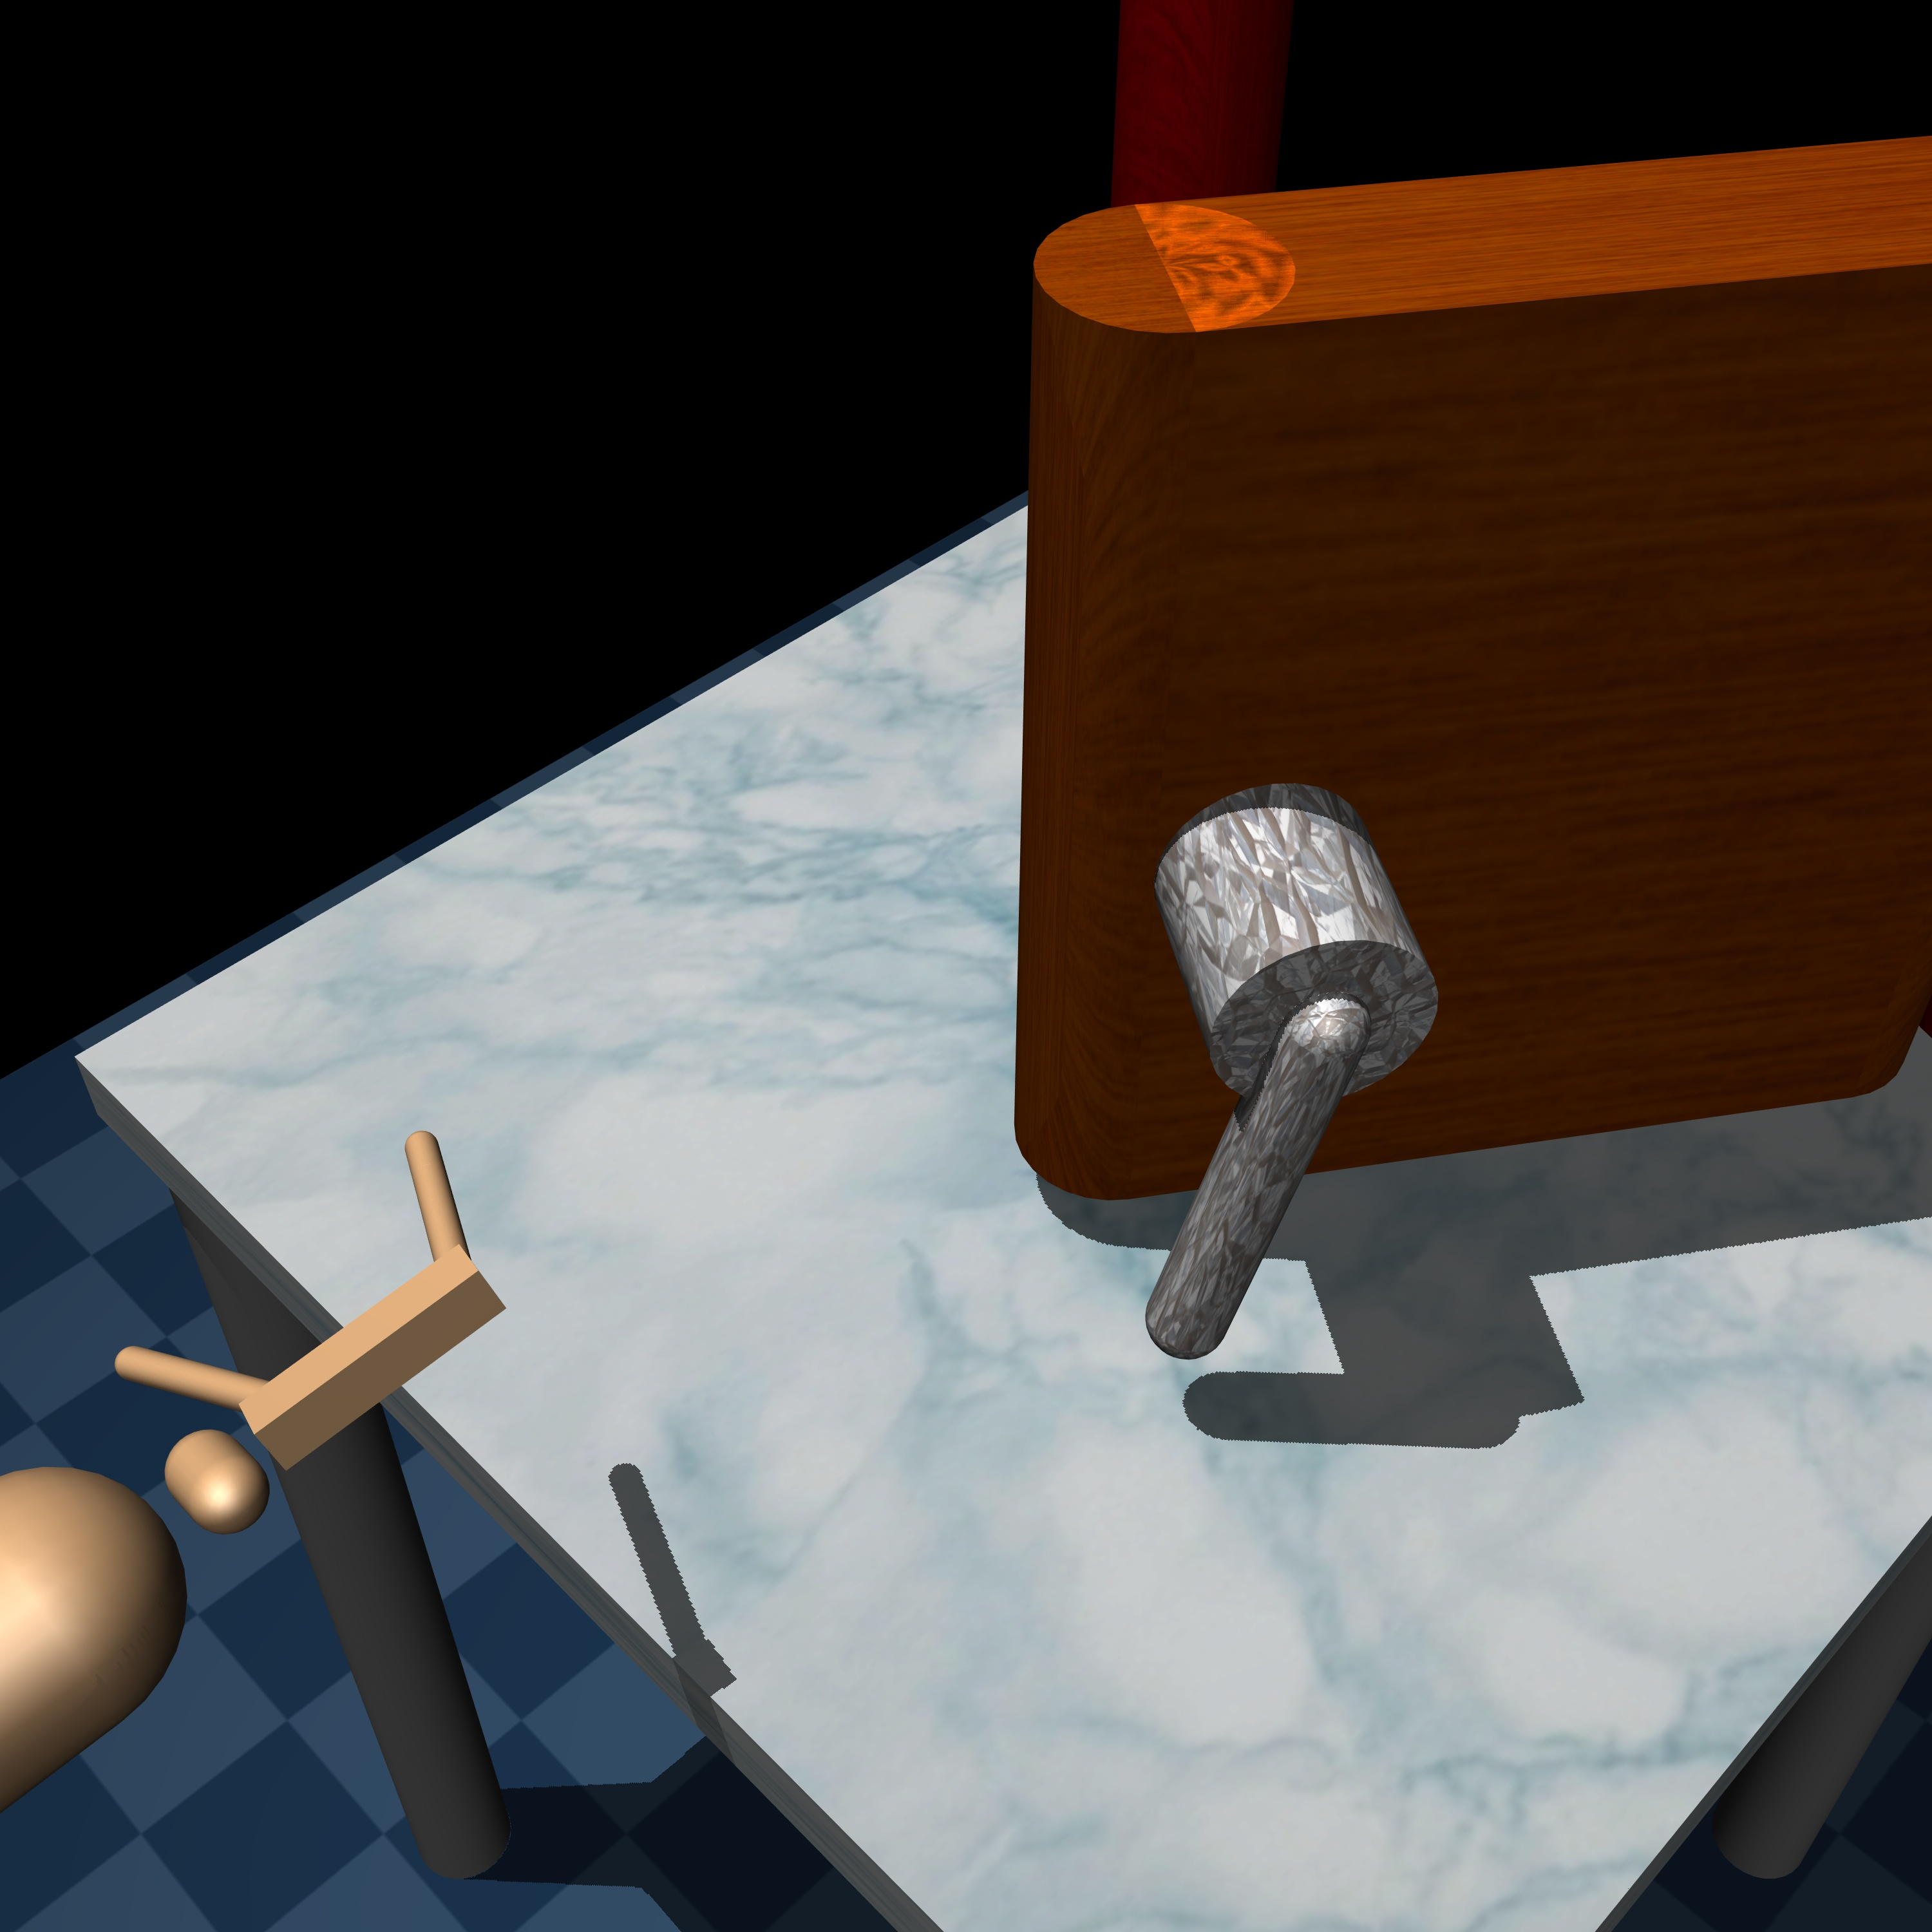
\includegraphics[width=\suppwidth\textwidth,valign=m]{Figures/supp/door/target/image-0080.jpg}
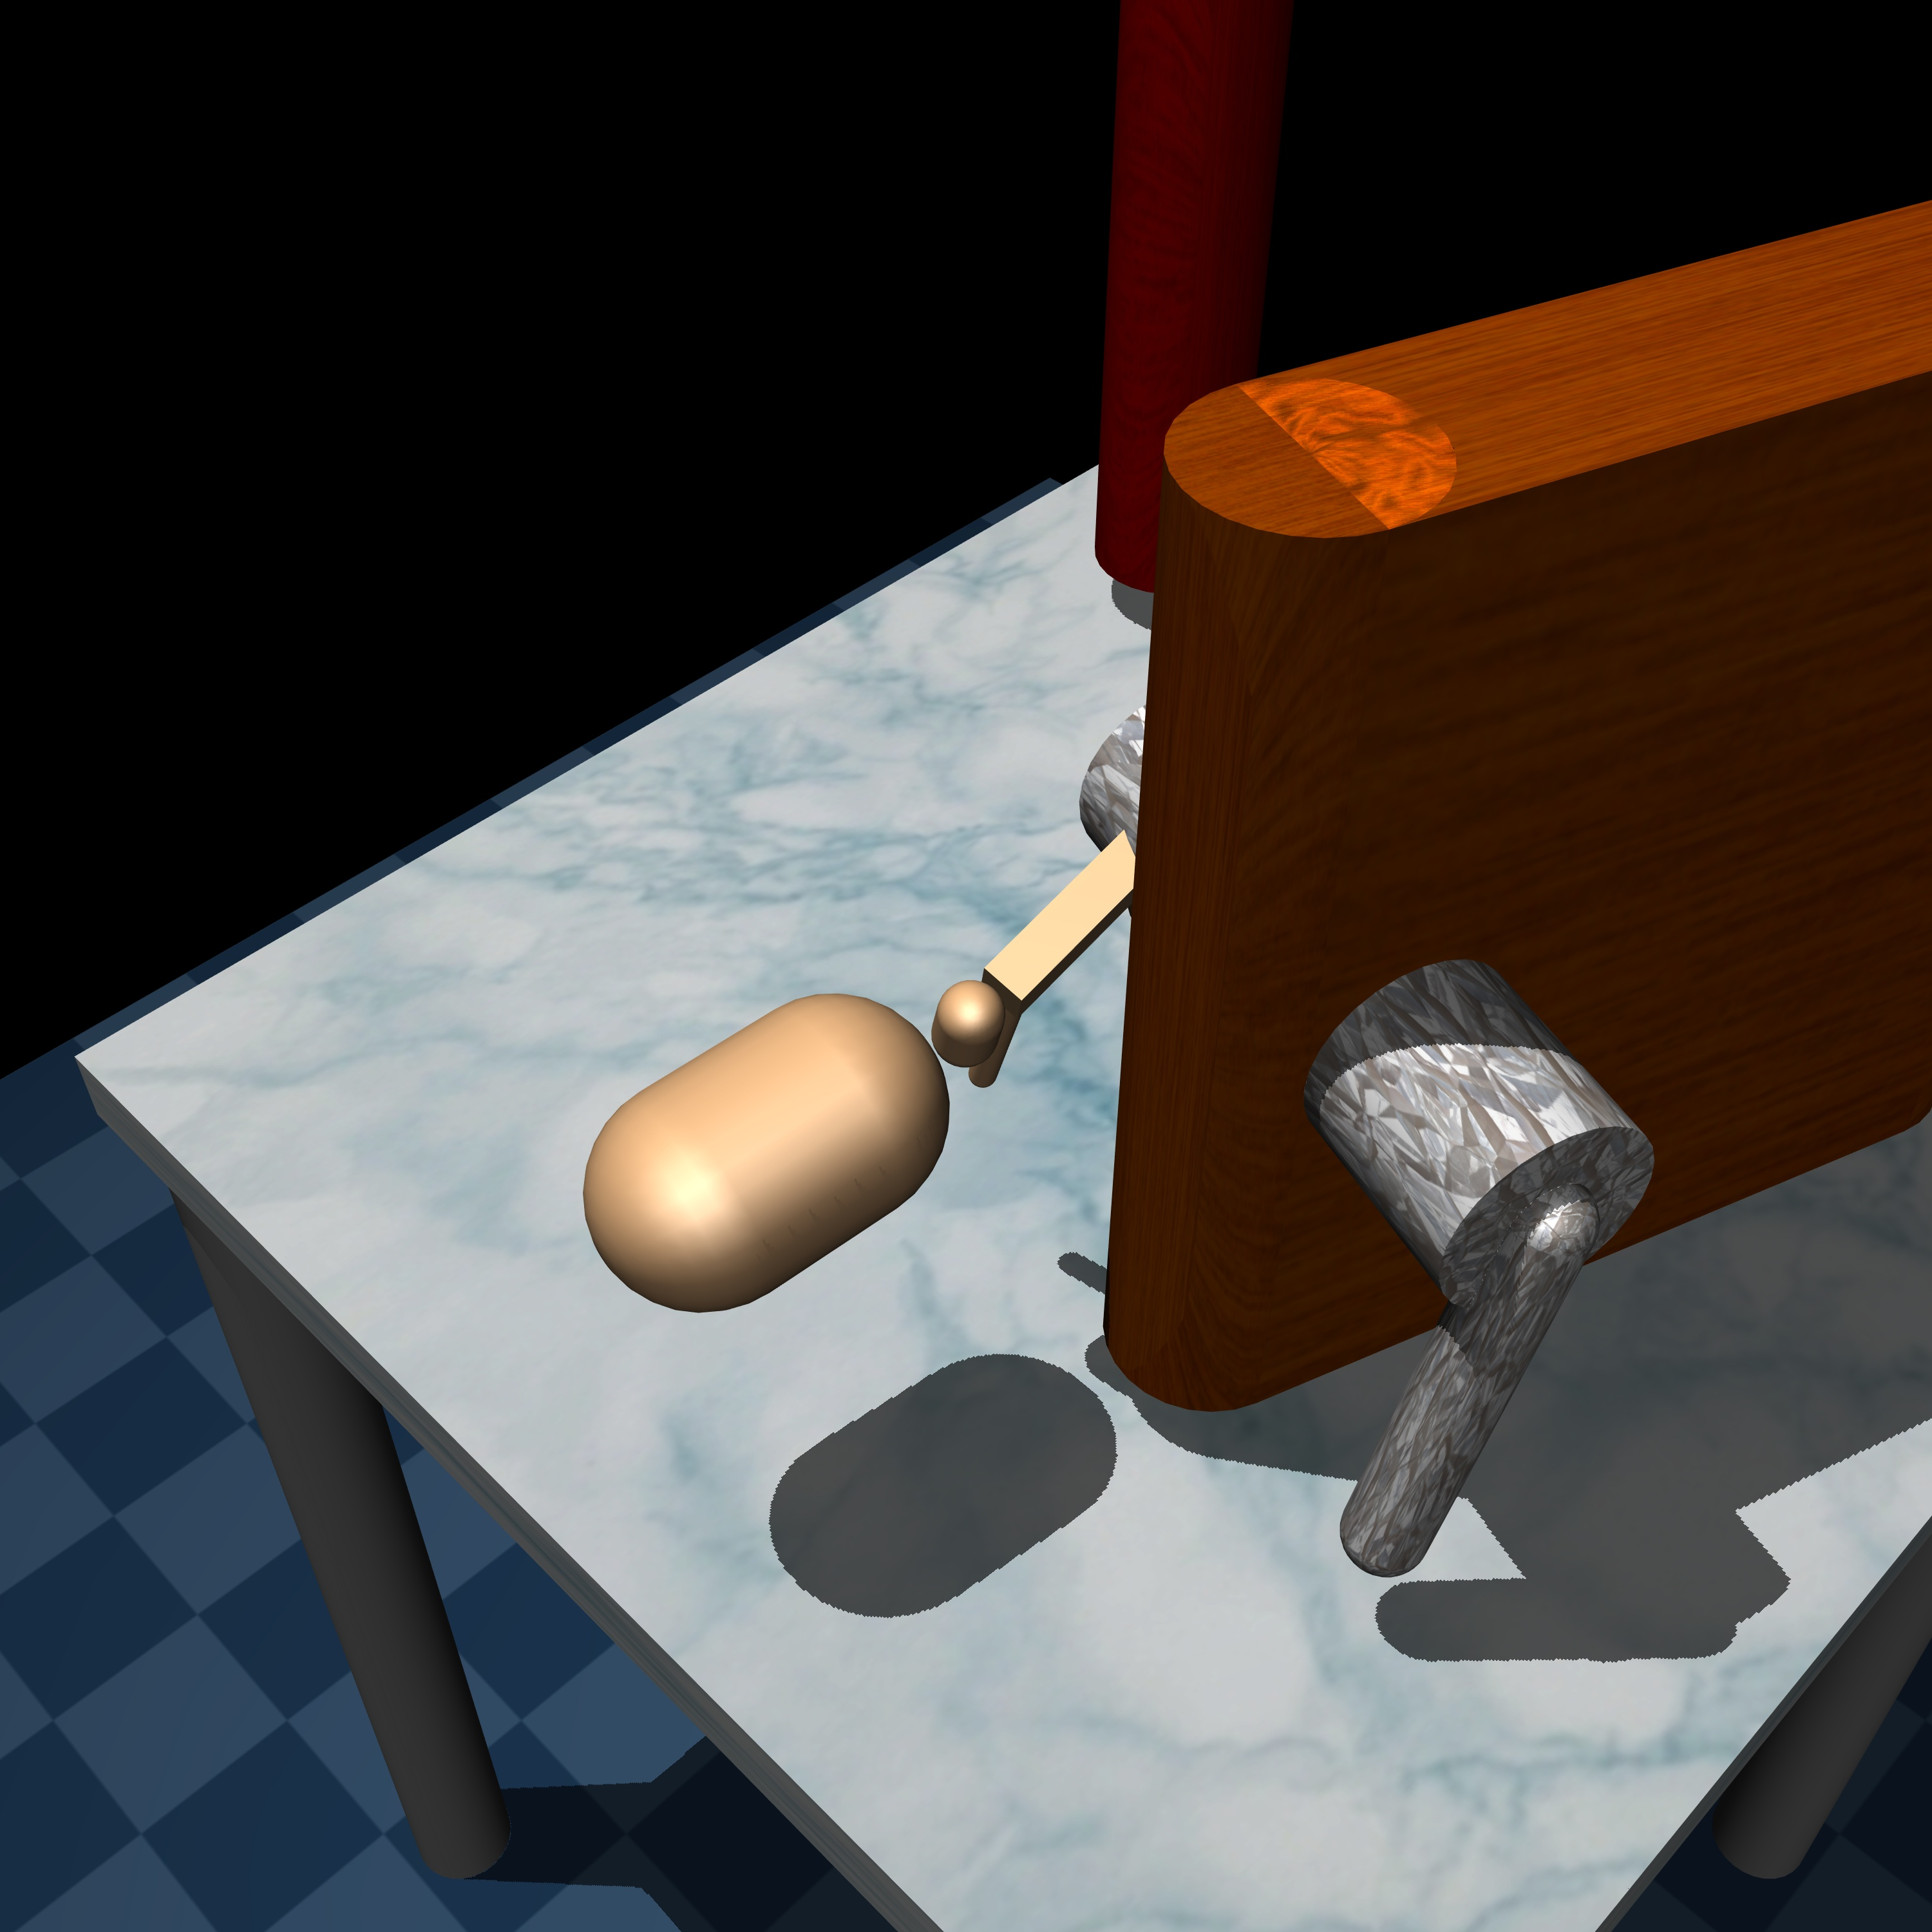
\includegraphics[width=\suppwidth\textwidth,valign=m]{Figures/supp/door/target/image-0100.jpg} \\ \\
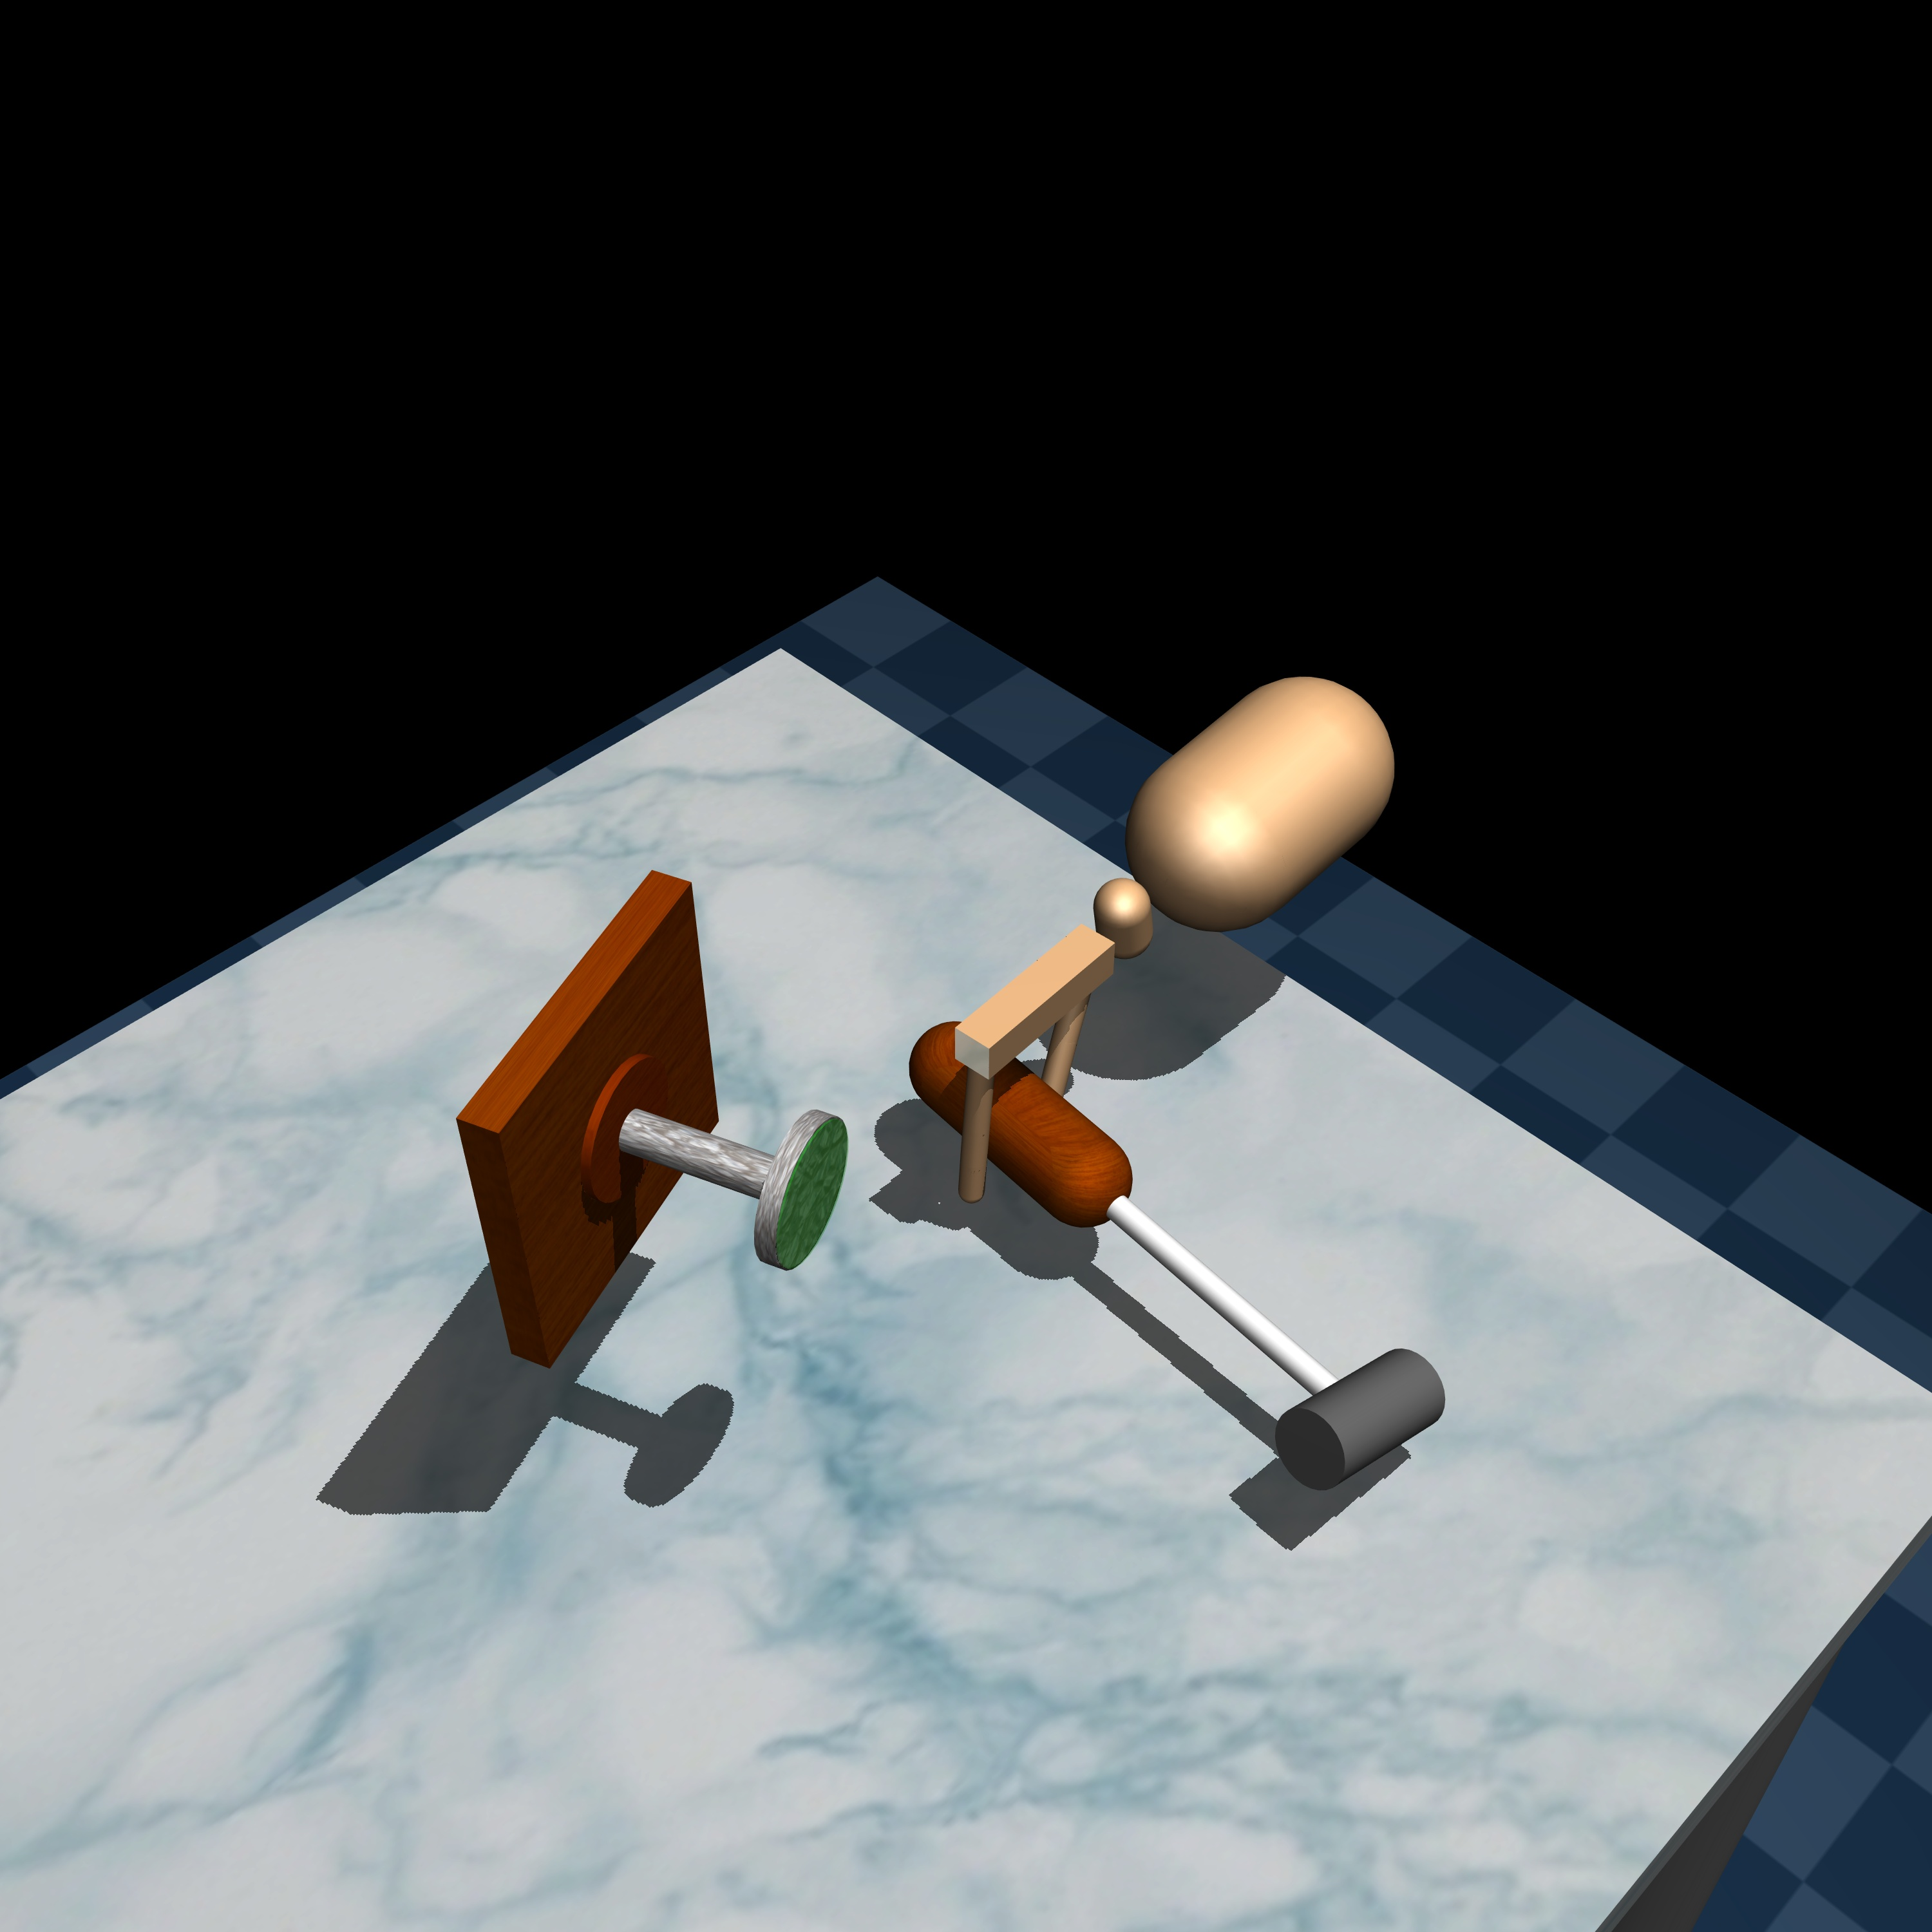
\includegraphics[width=\suppwidth\textwidth, valign=m]{Figures/supp/hammer/target/image-0018.jpg}
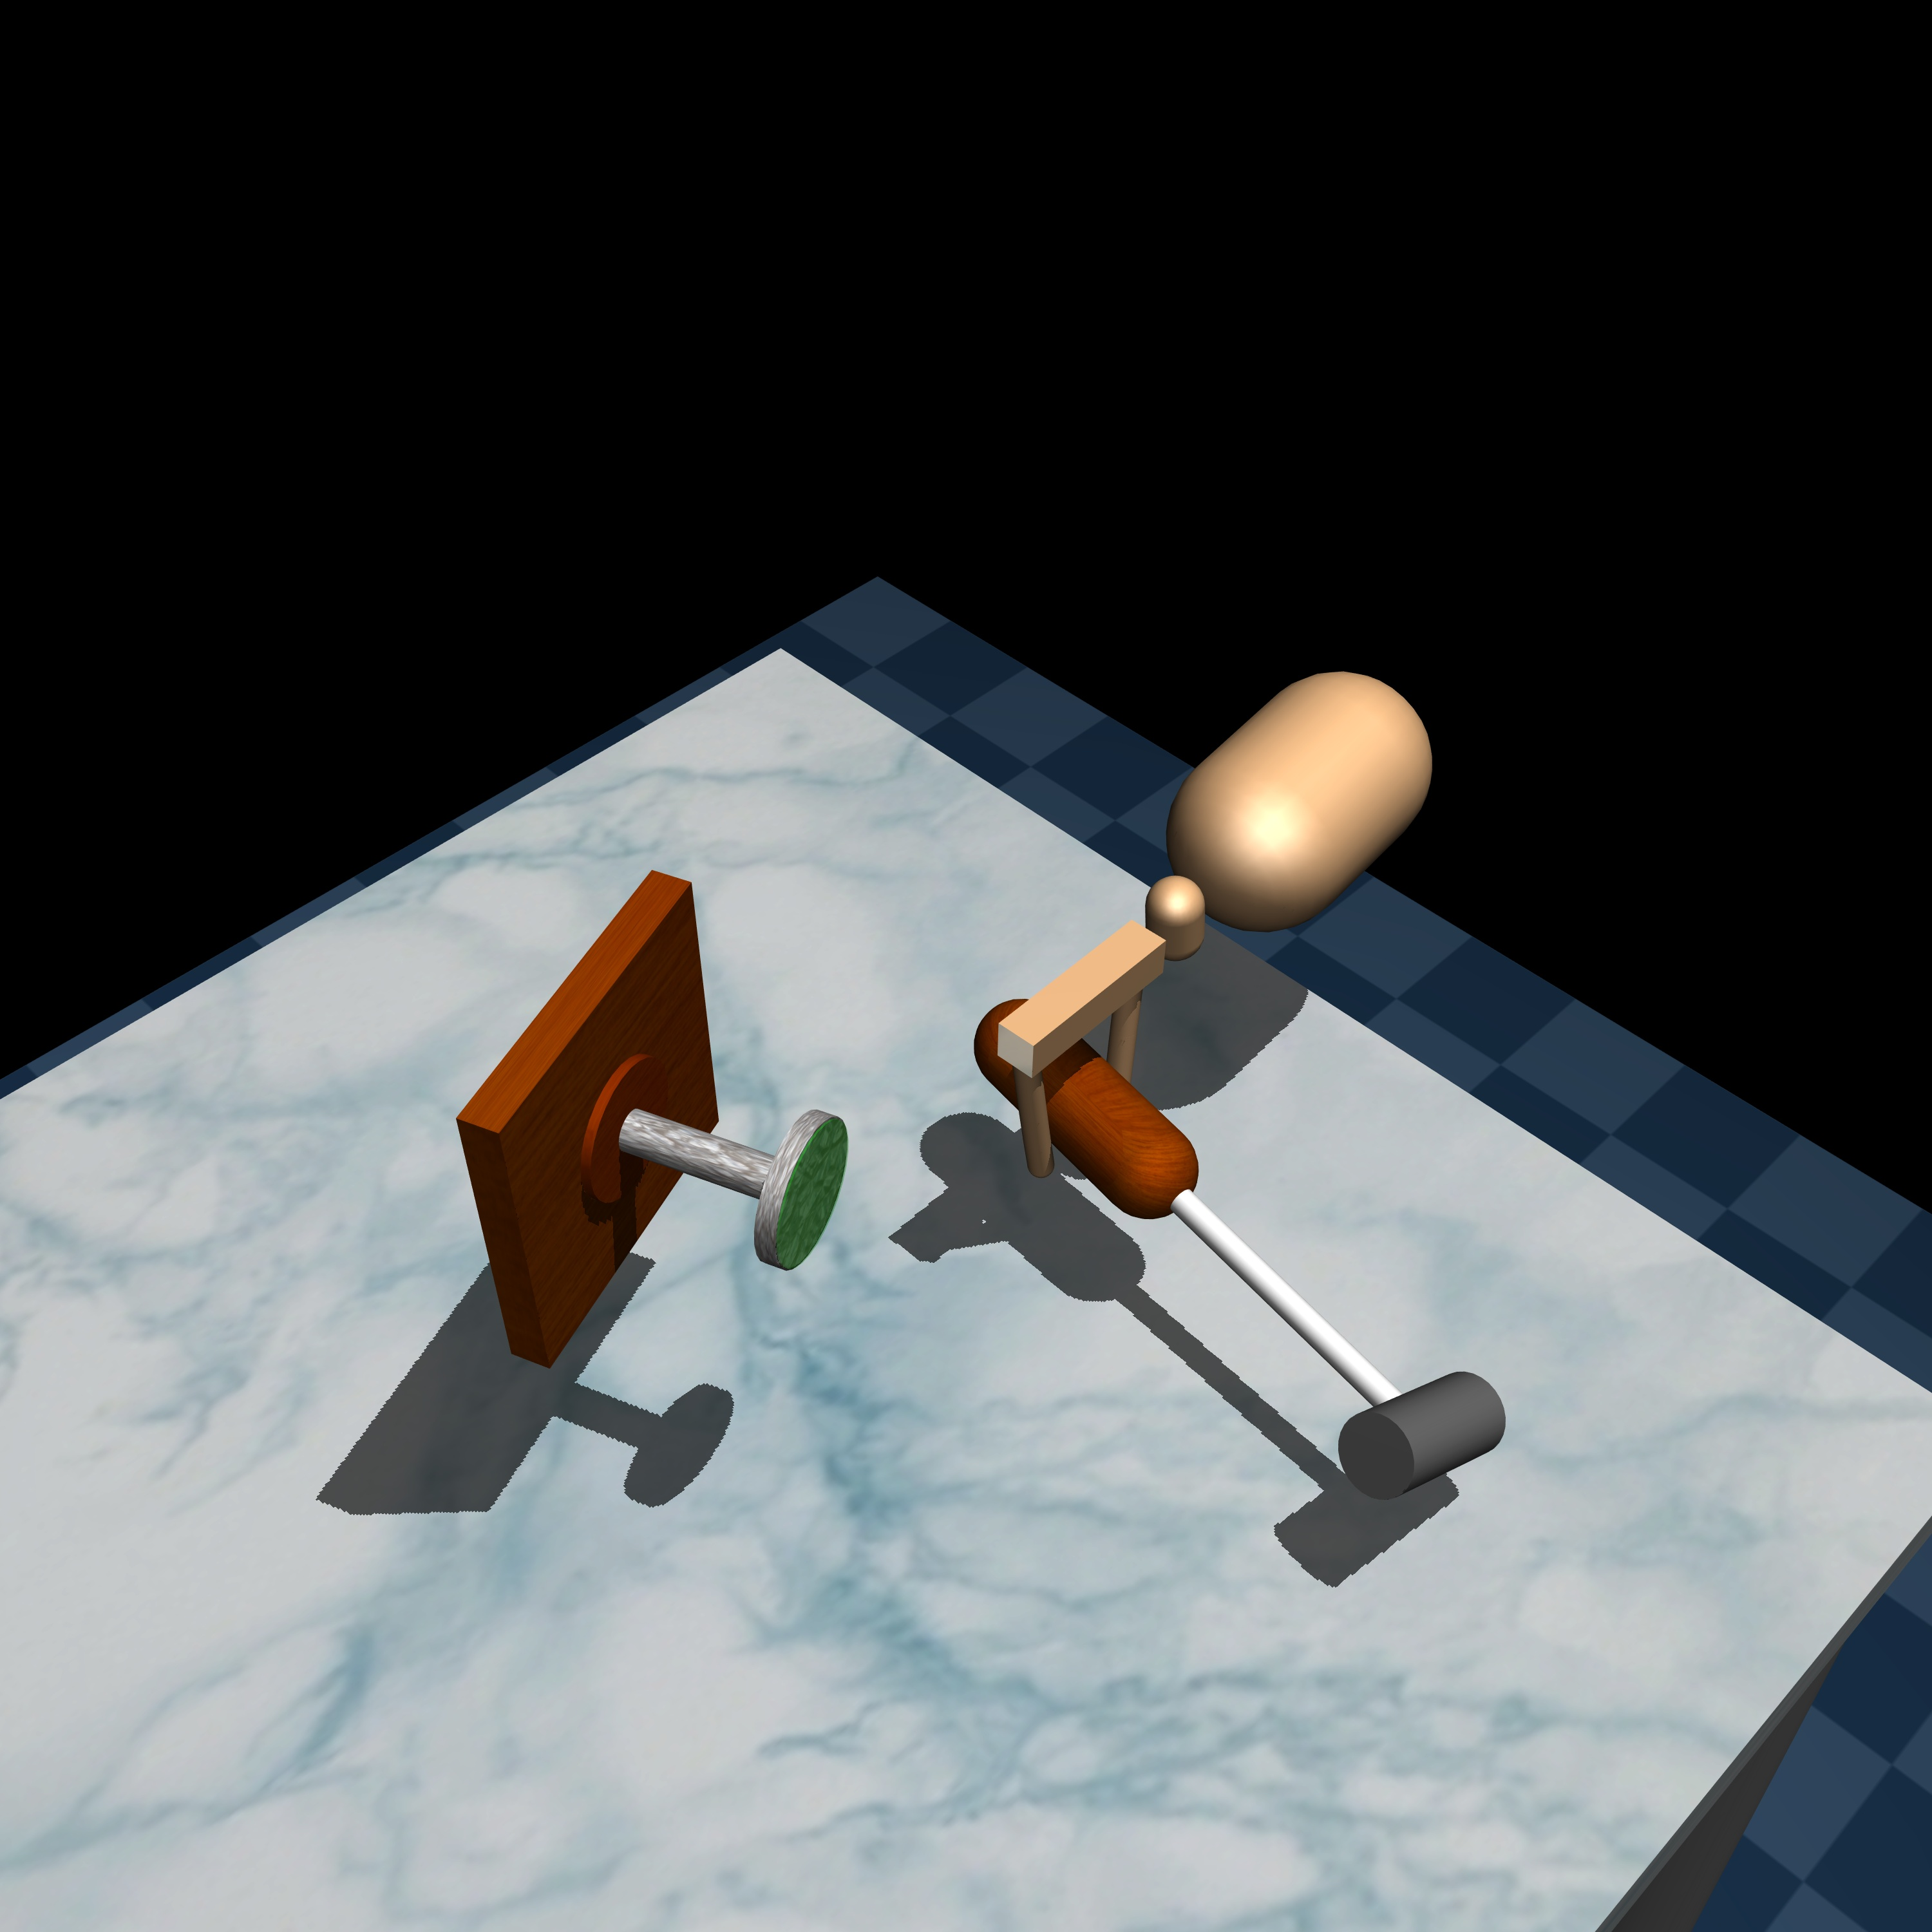
\includegraphics[width=\suppwidth\textwidth,valign=m]{Figures/supp/hammer/target/image-0028.jpg}
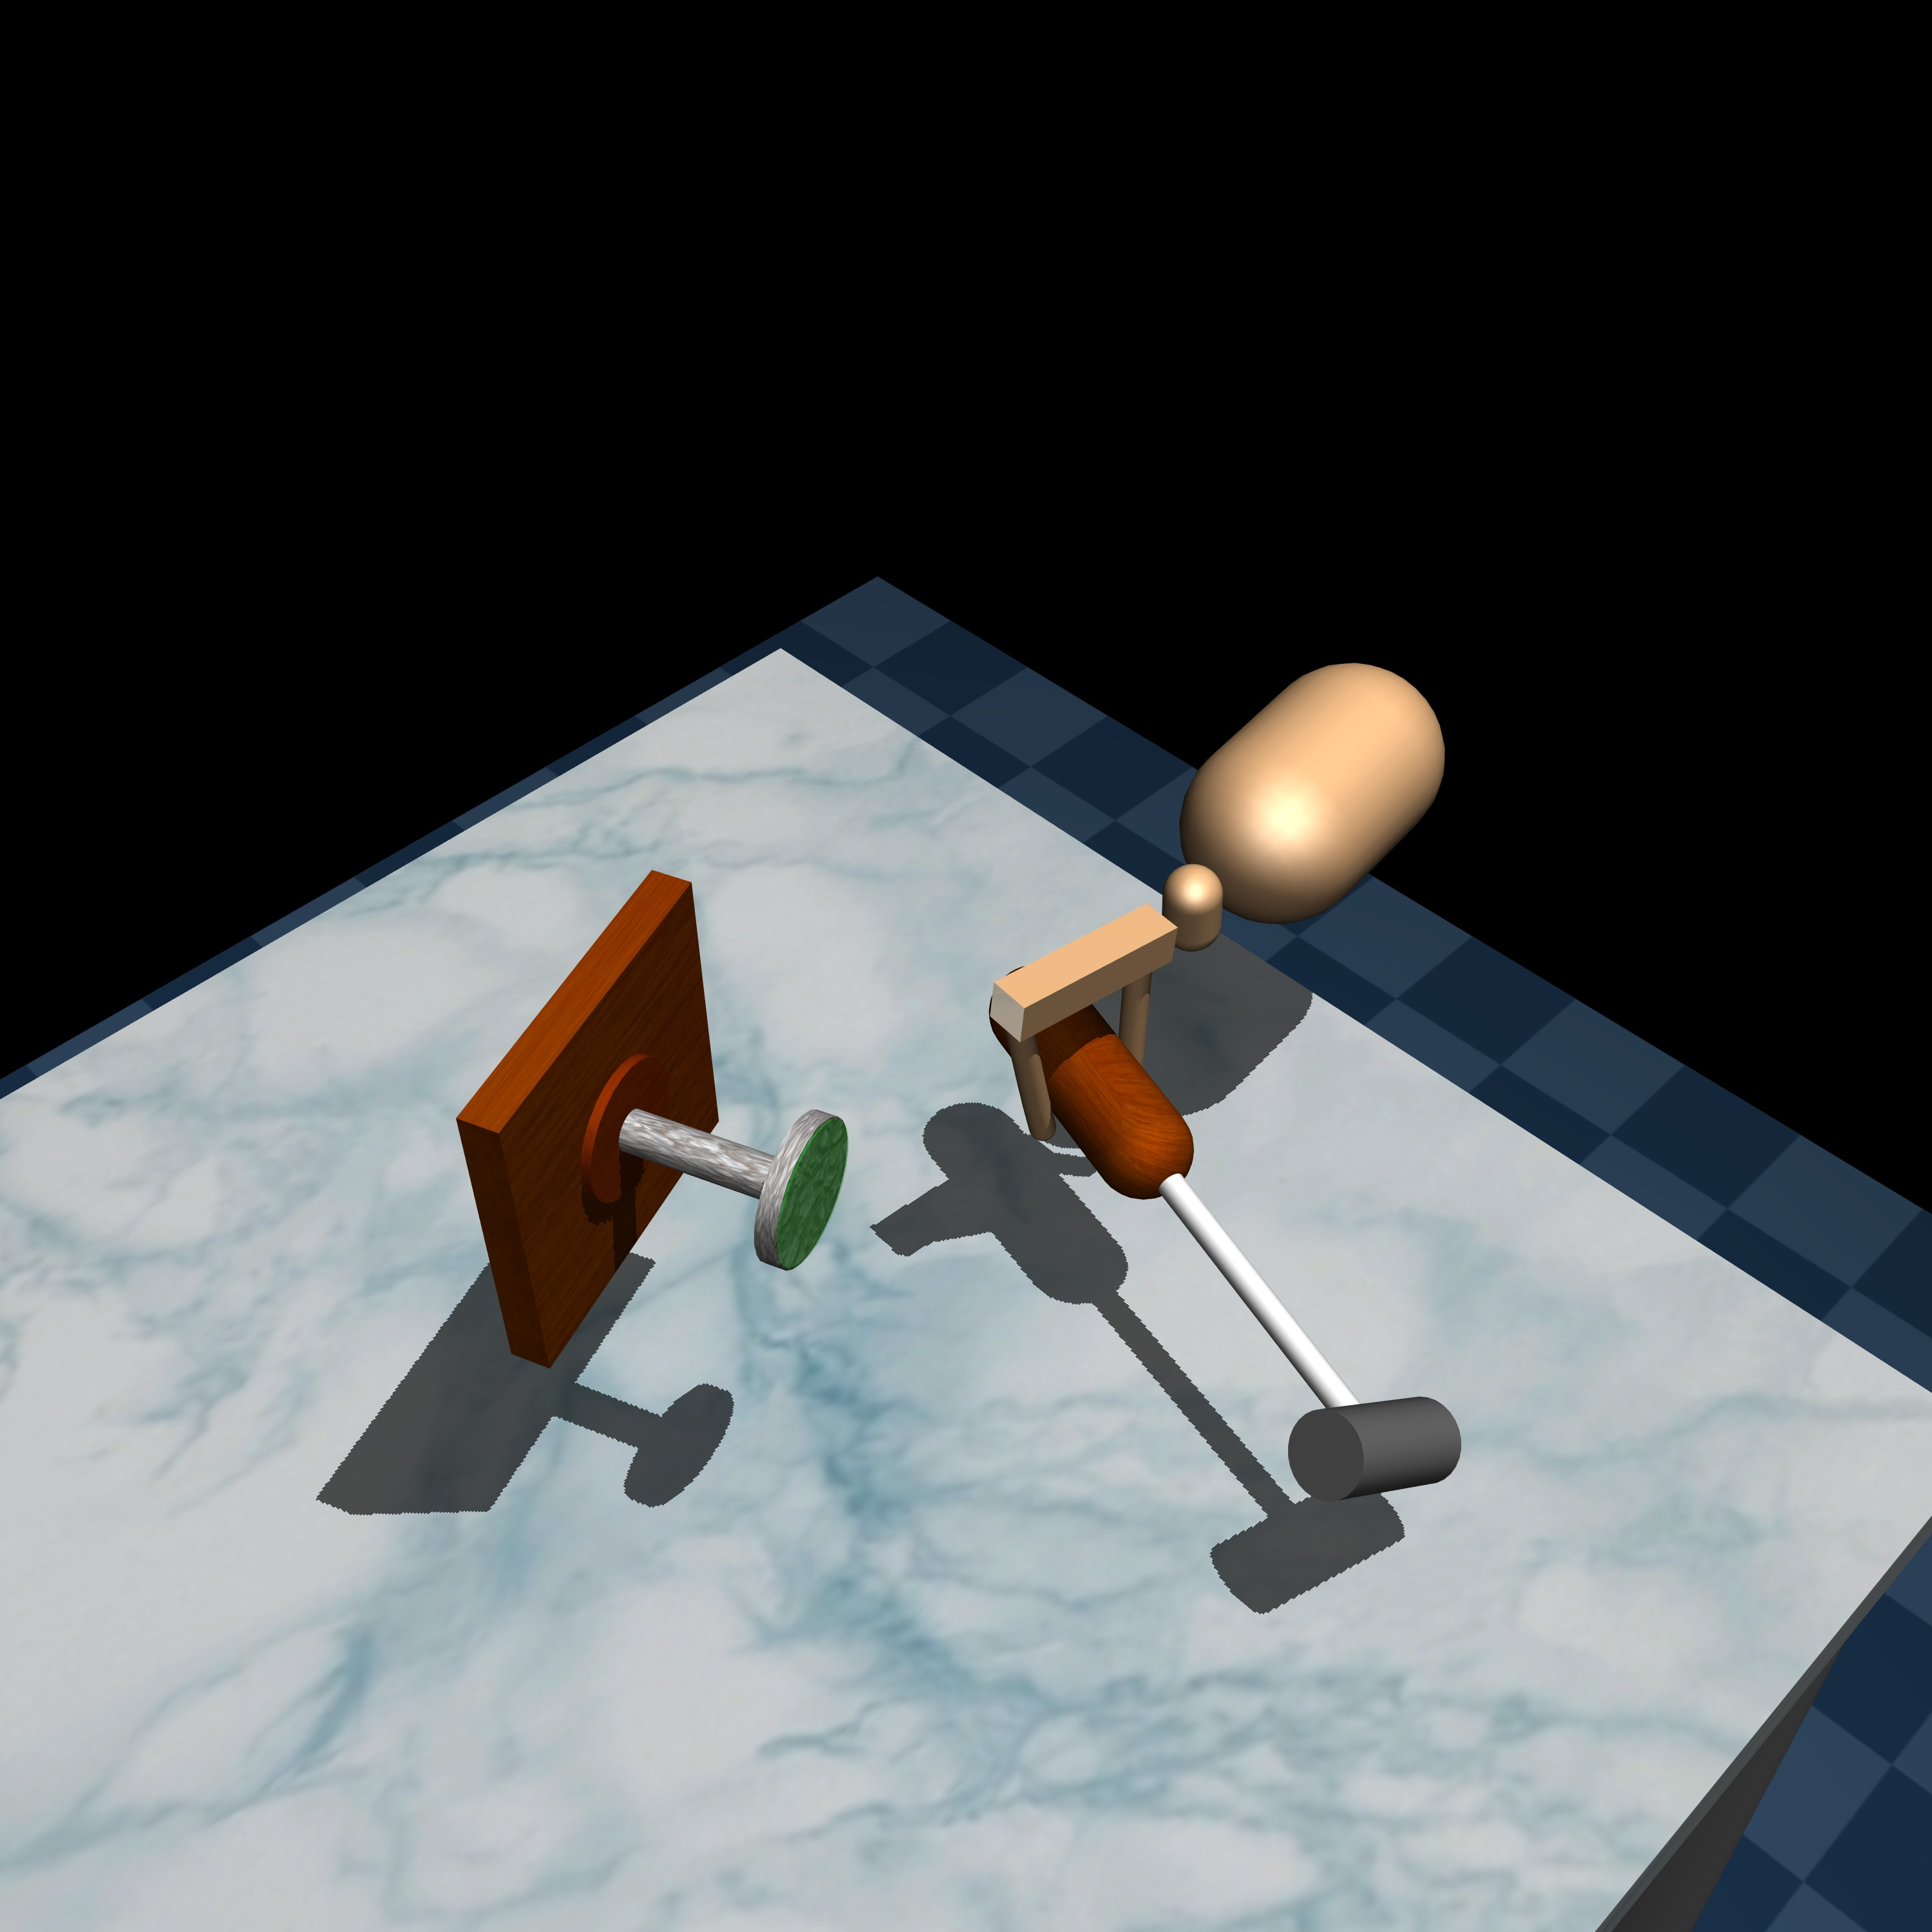
\includegraphics[width=\suppwidth\textwidth,valign=m]{Figures/supp/hammer/target/image-0038.jpg}
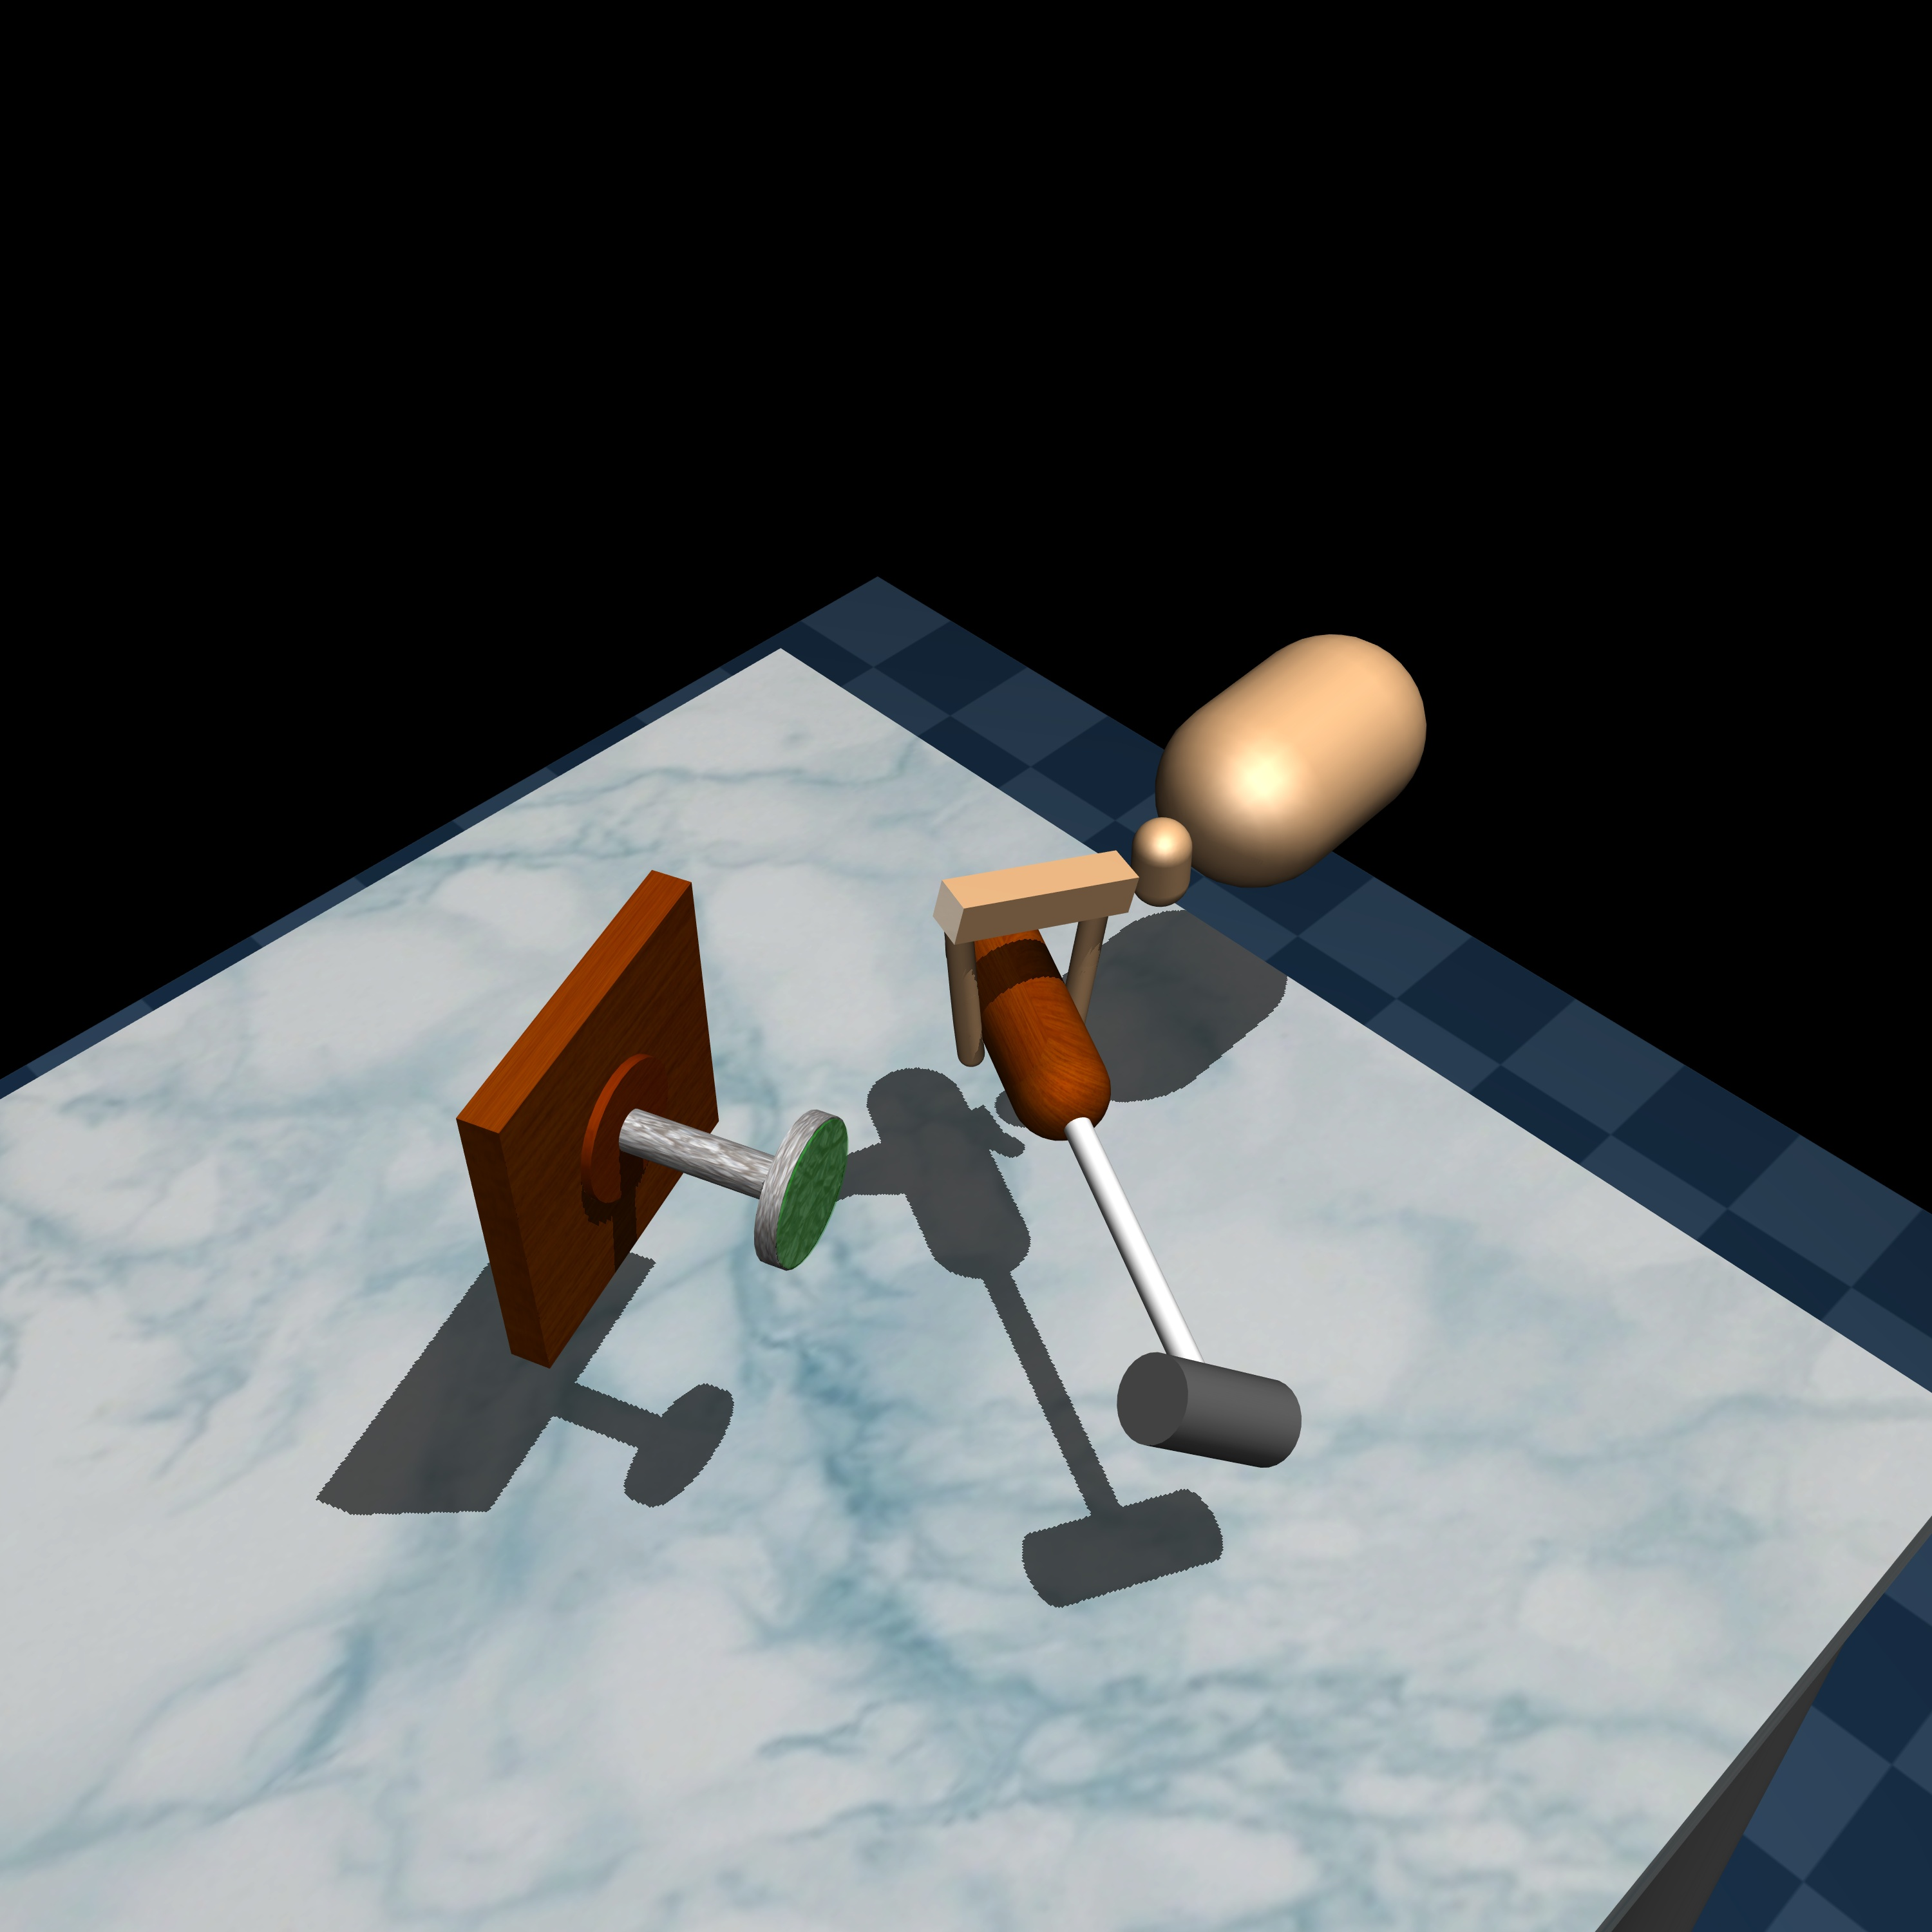
\includegraphics[width=\suppwidth\textwidth, valign=m]{Figures/supp/hammer/target/image-0048.jpg}
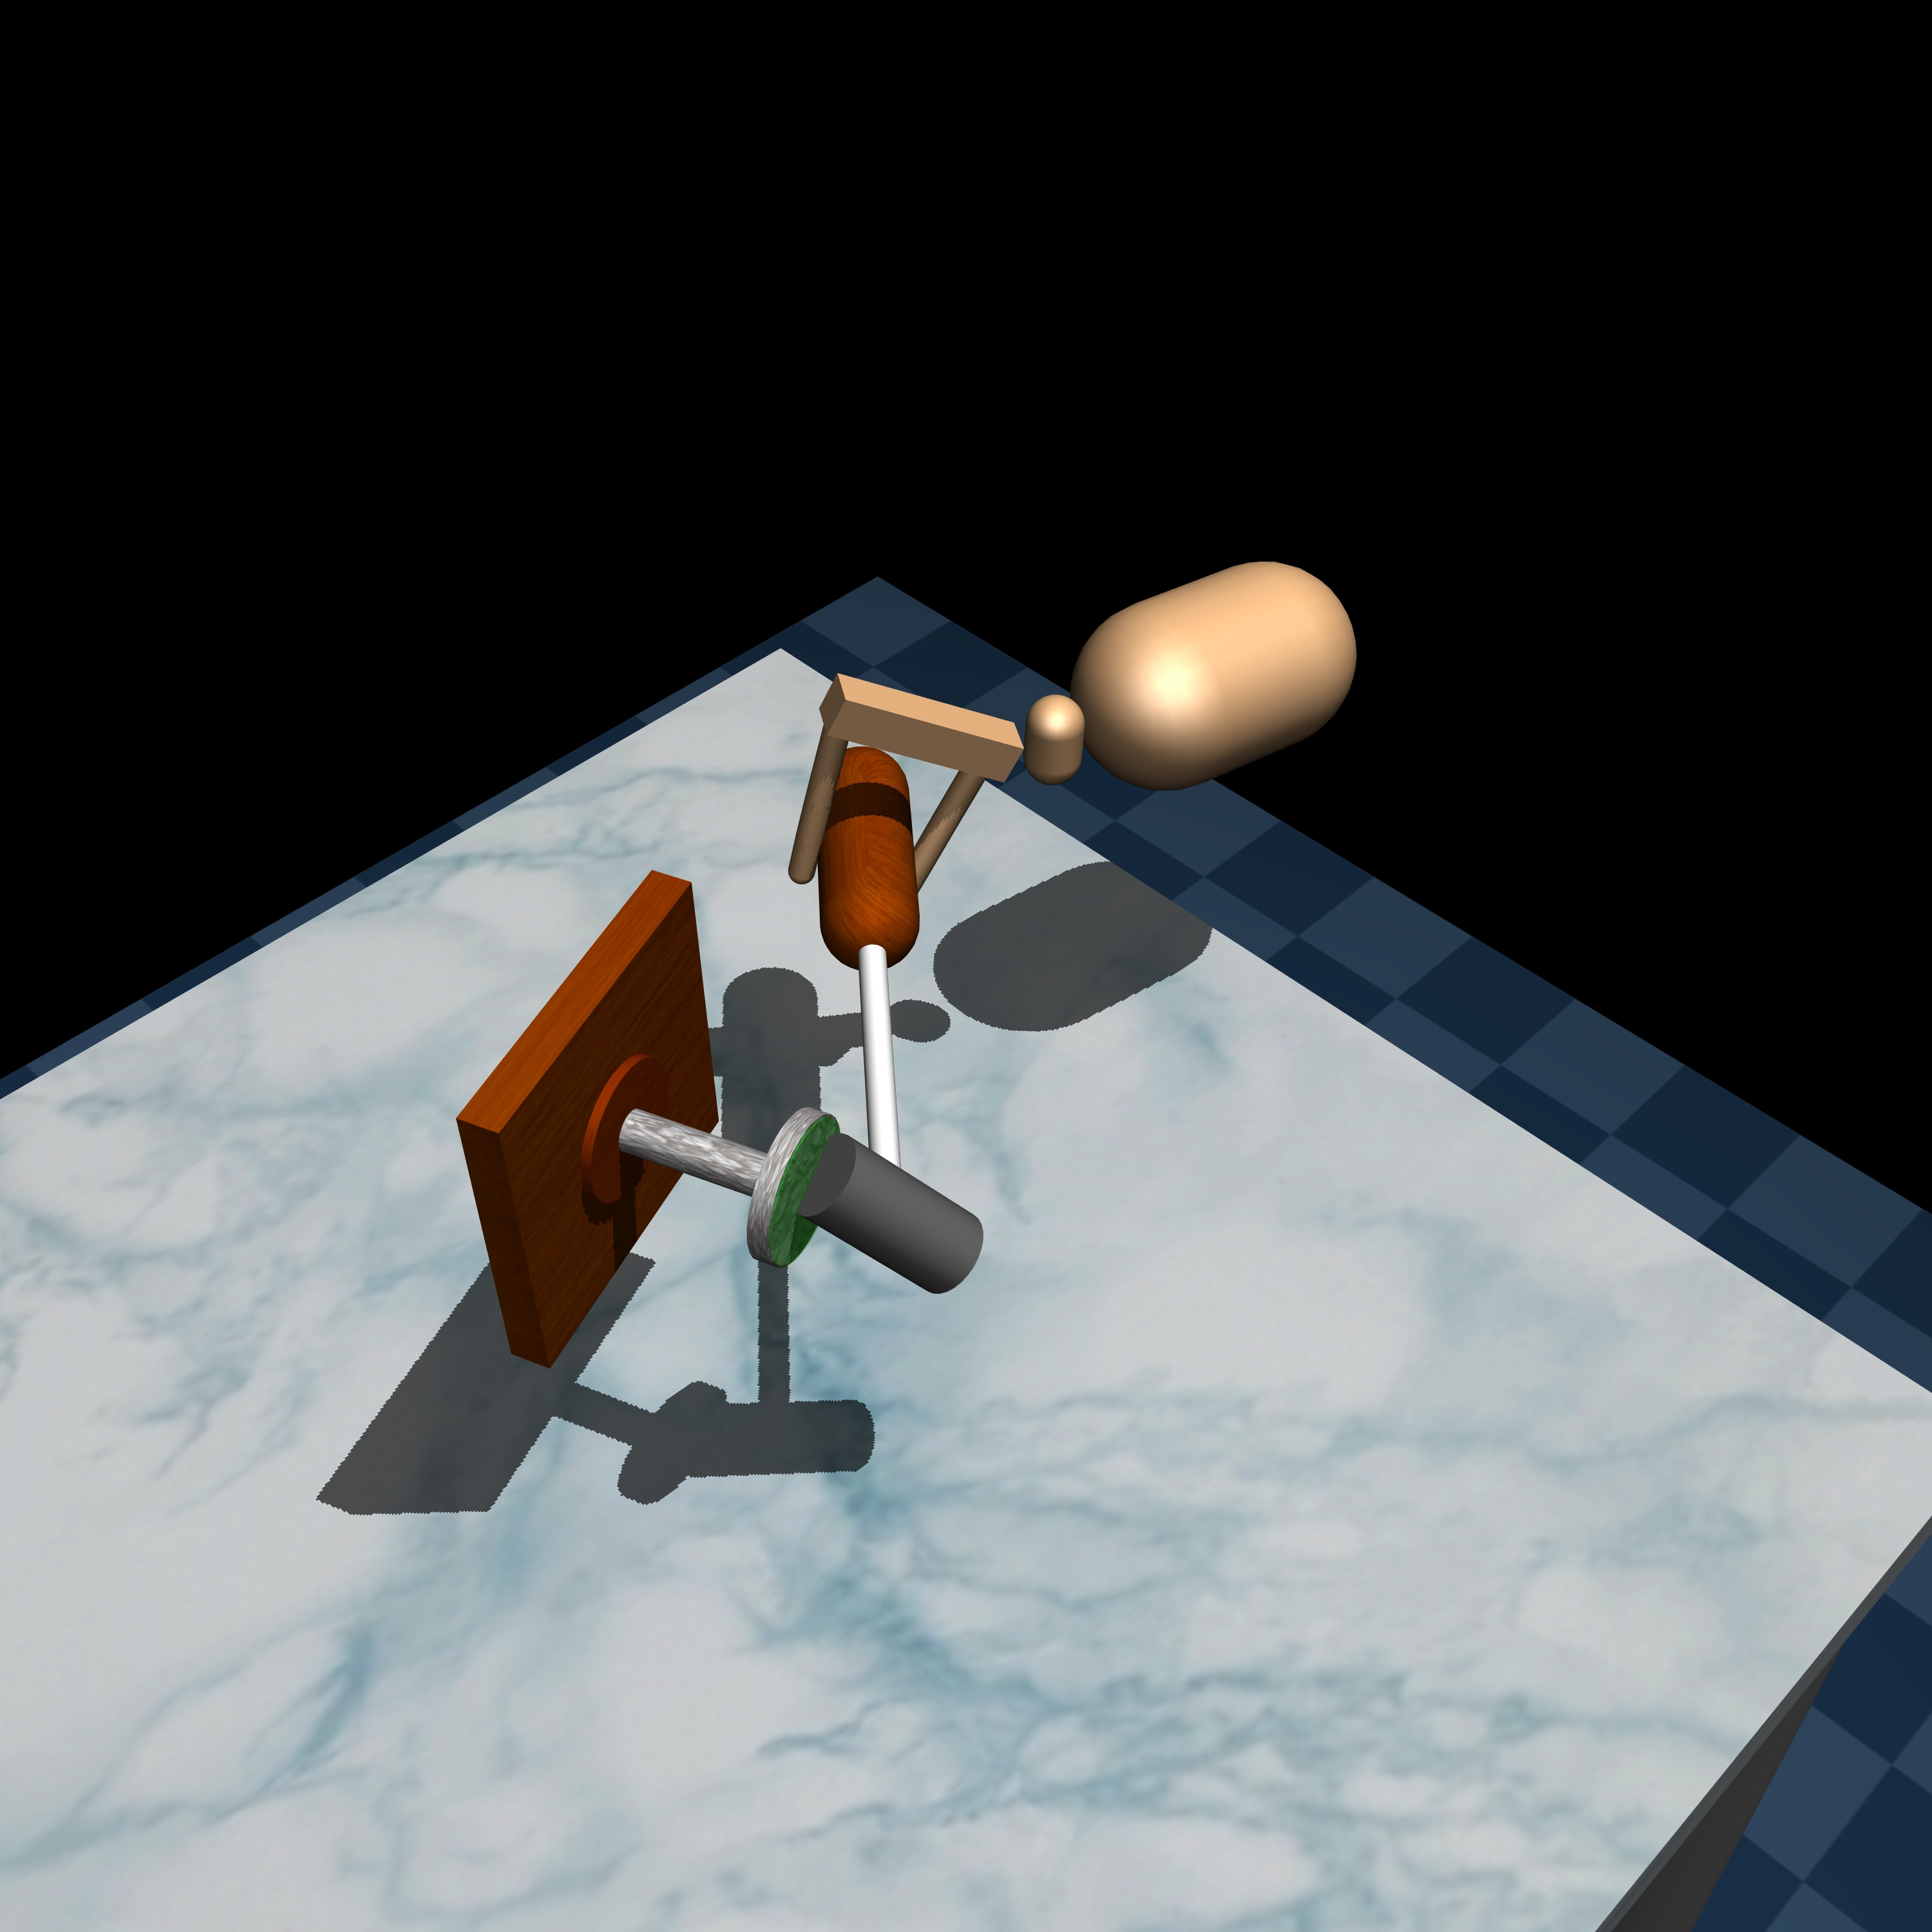
\includegraphics[width=\suppwidth\textwidth,valign=m]{Figures/supp/hammer/target/image-0058.jpg}
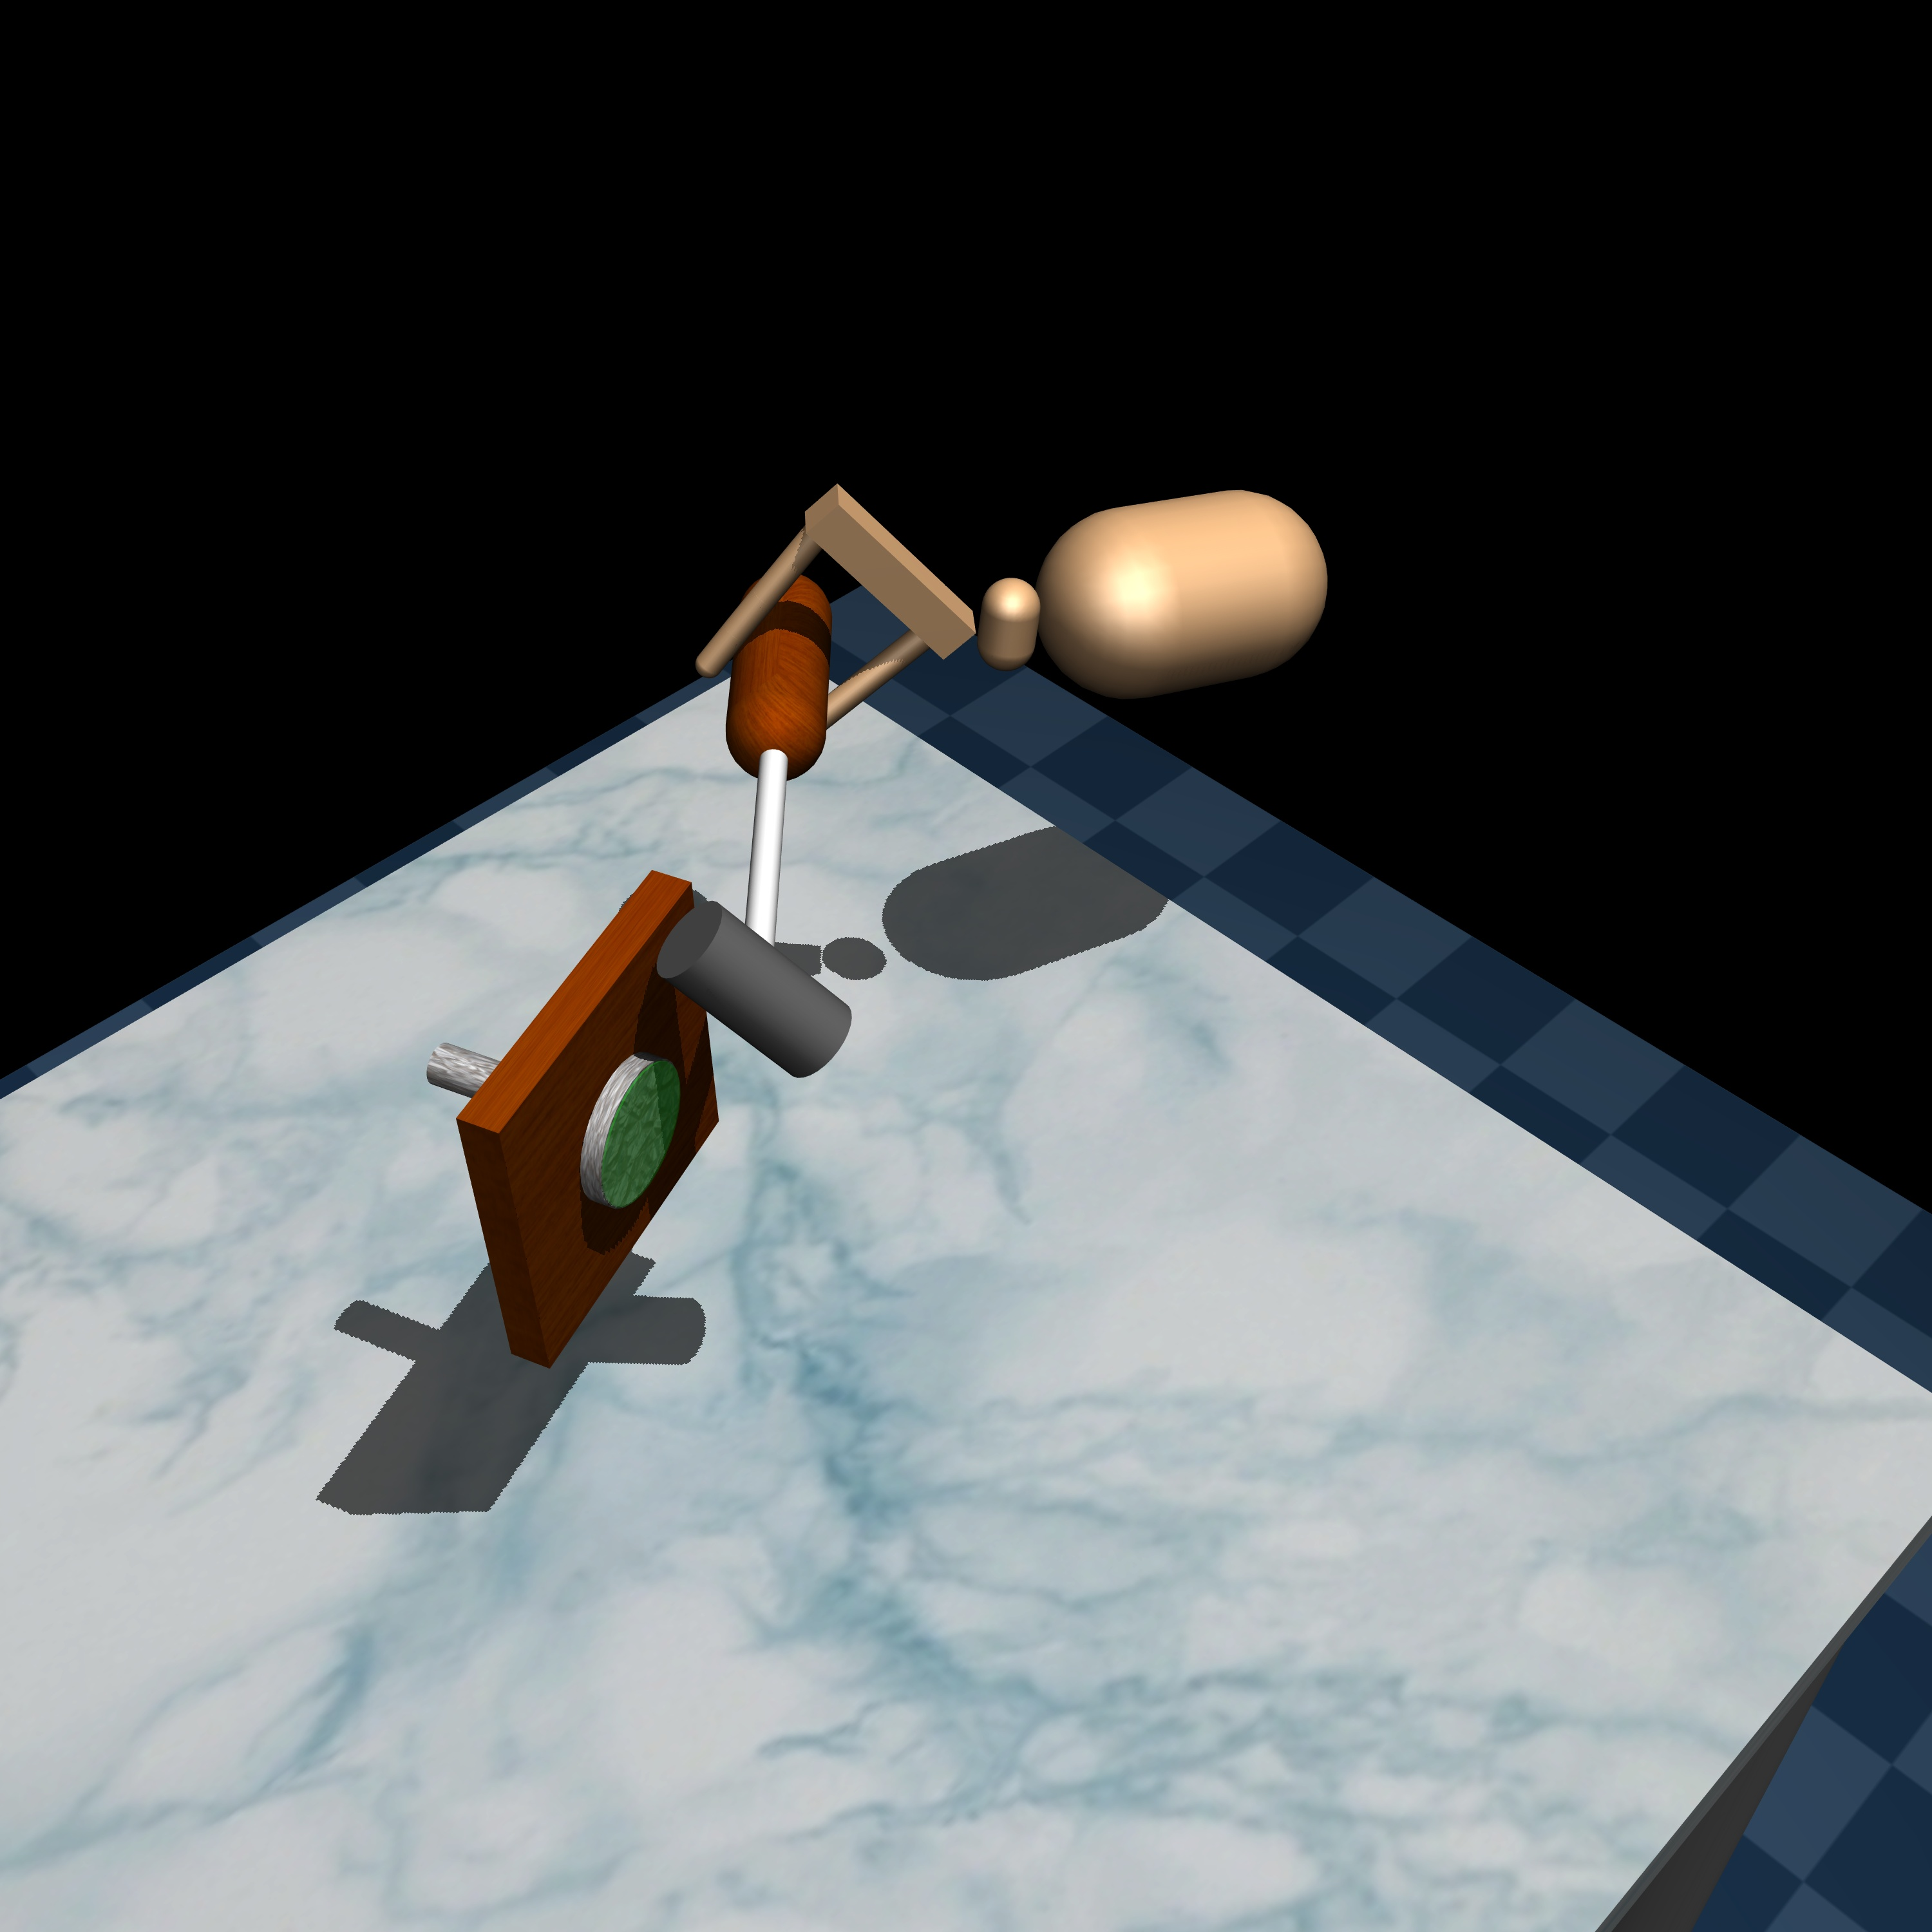
\includegraphics[width=\suppwidth\textwidth,valign=m]{Figures/supp/hammer/target/image-0068.jpg} \\ \\
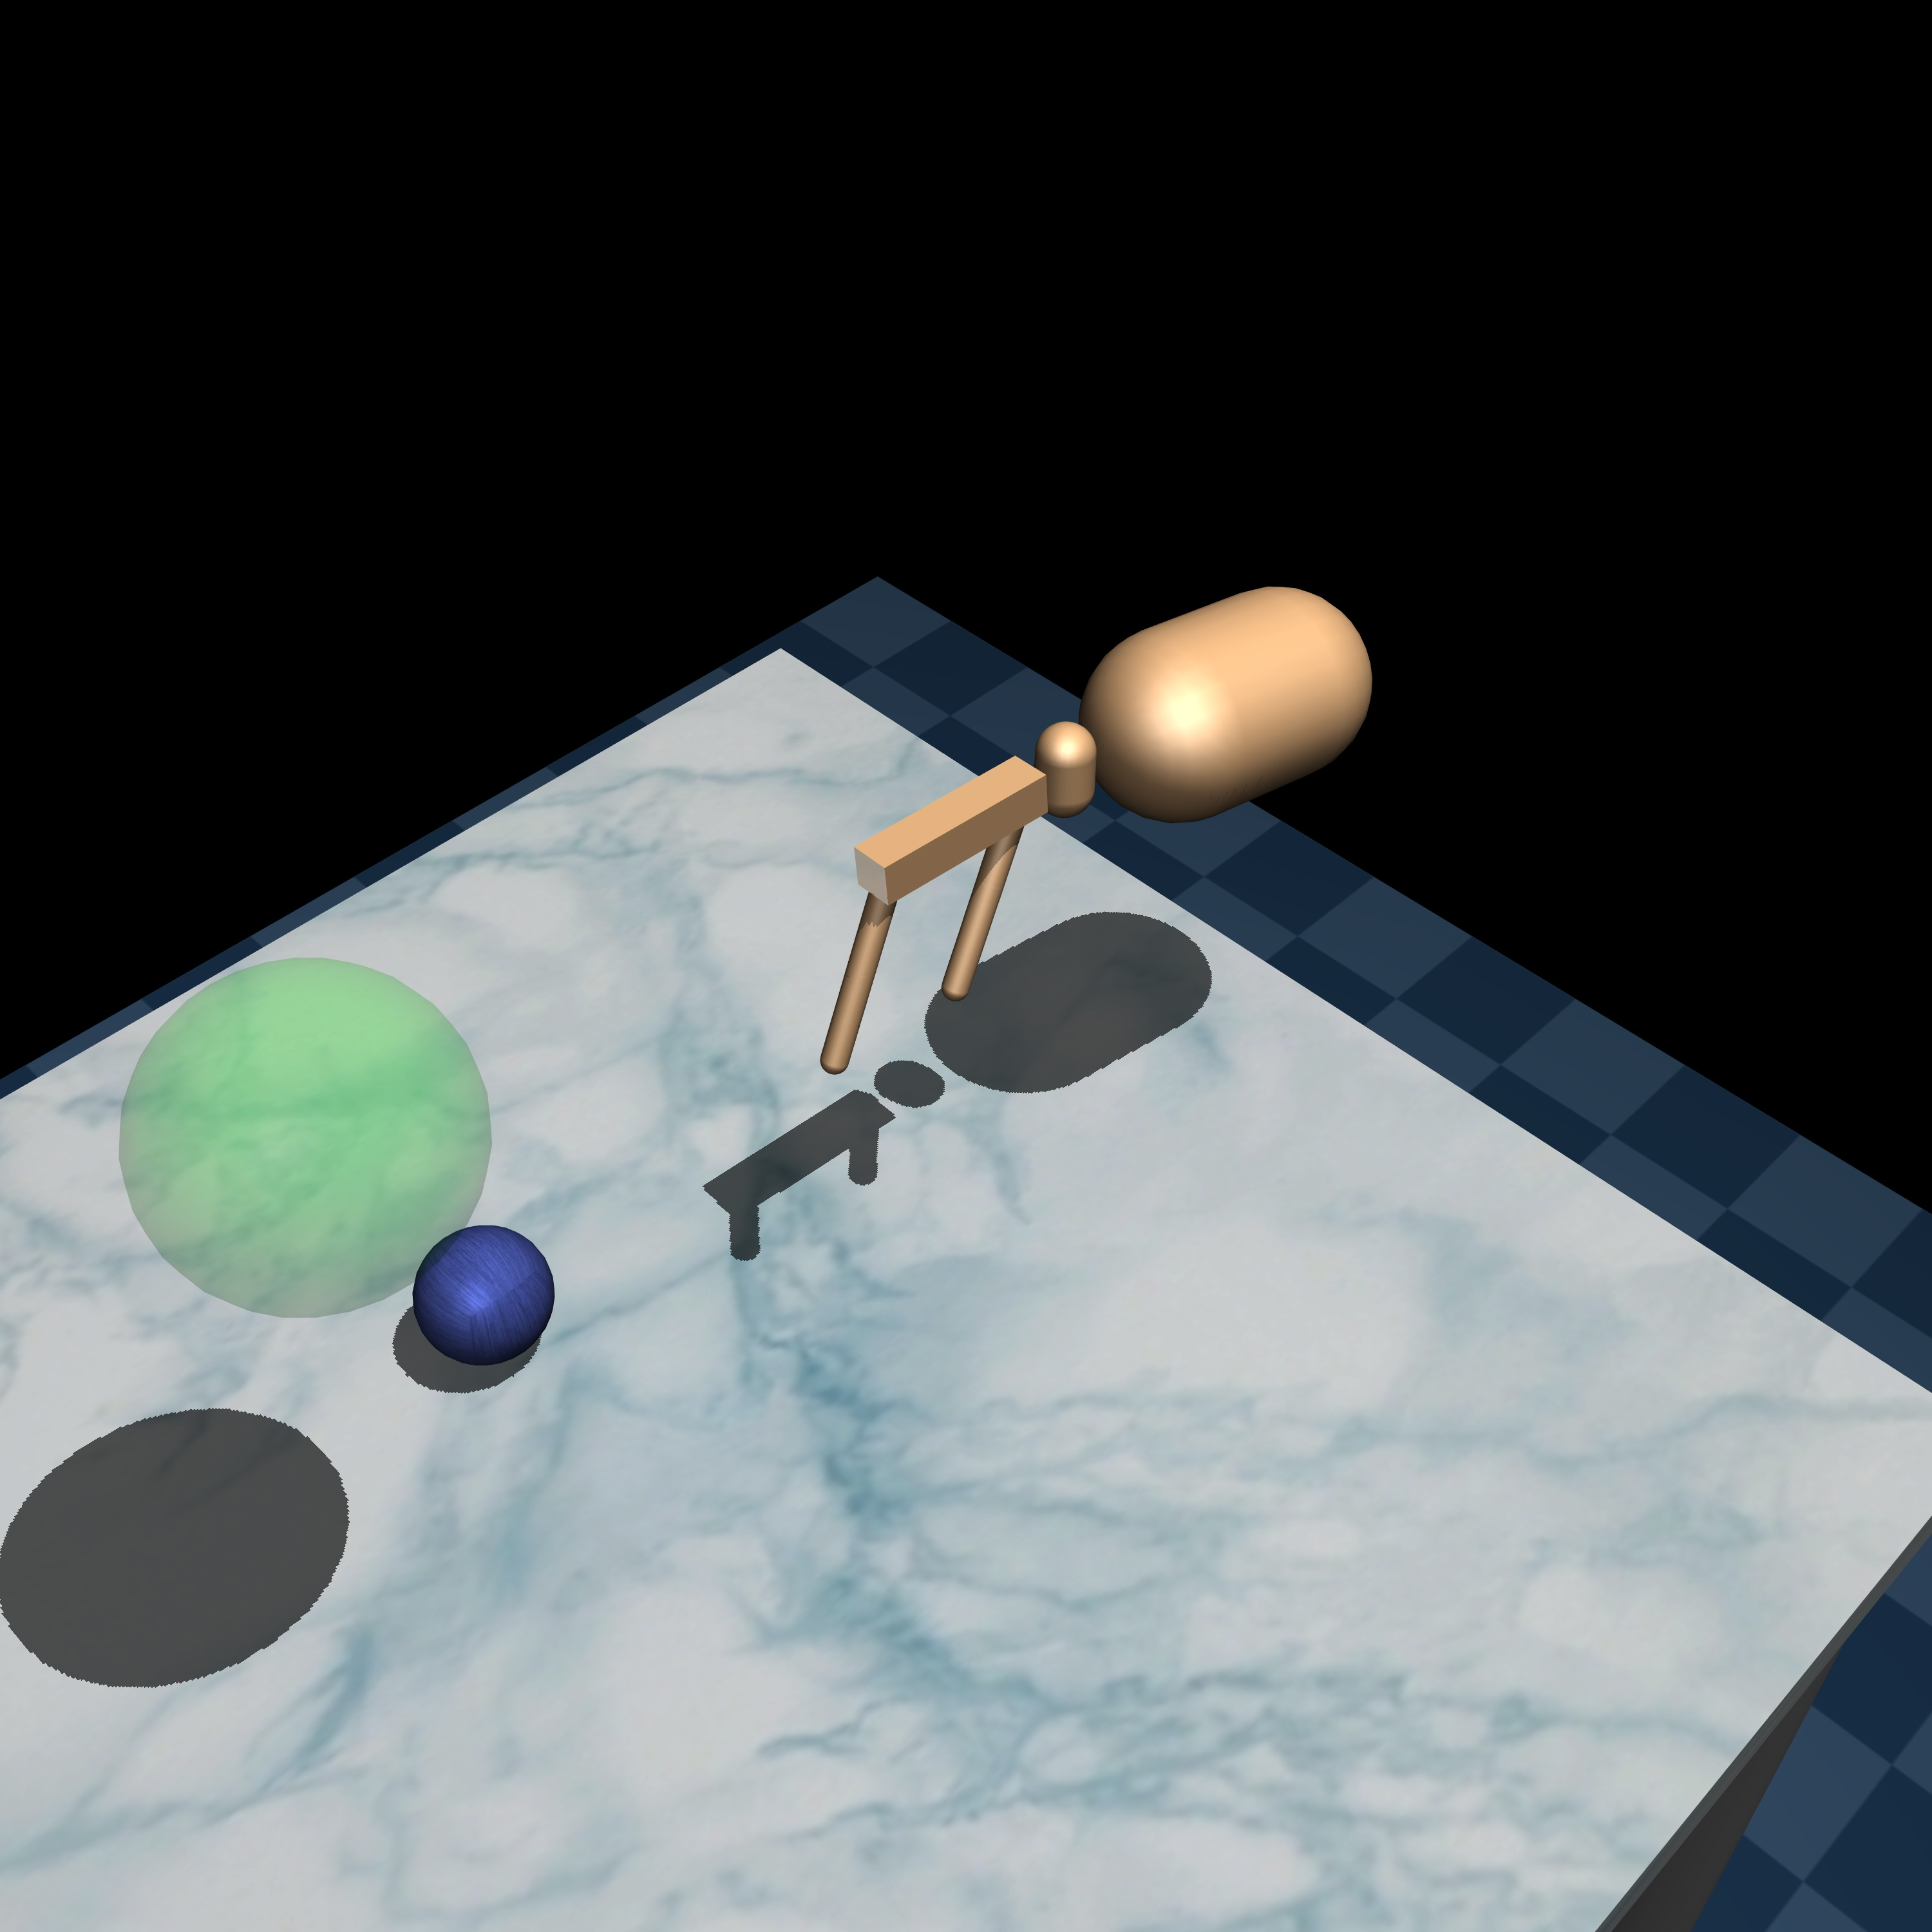
\includegraphics[width=\suppwidth\textwidth,valign=m]{Figures/supp/relocate/target/image-0006.jpg}
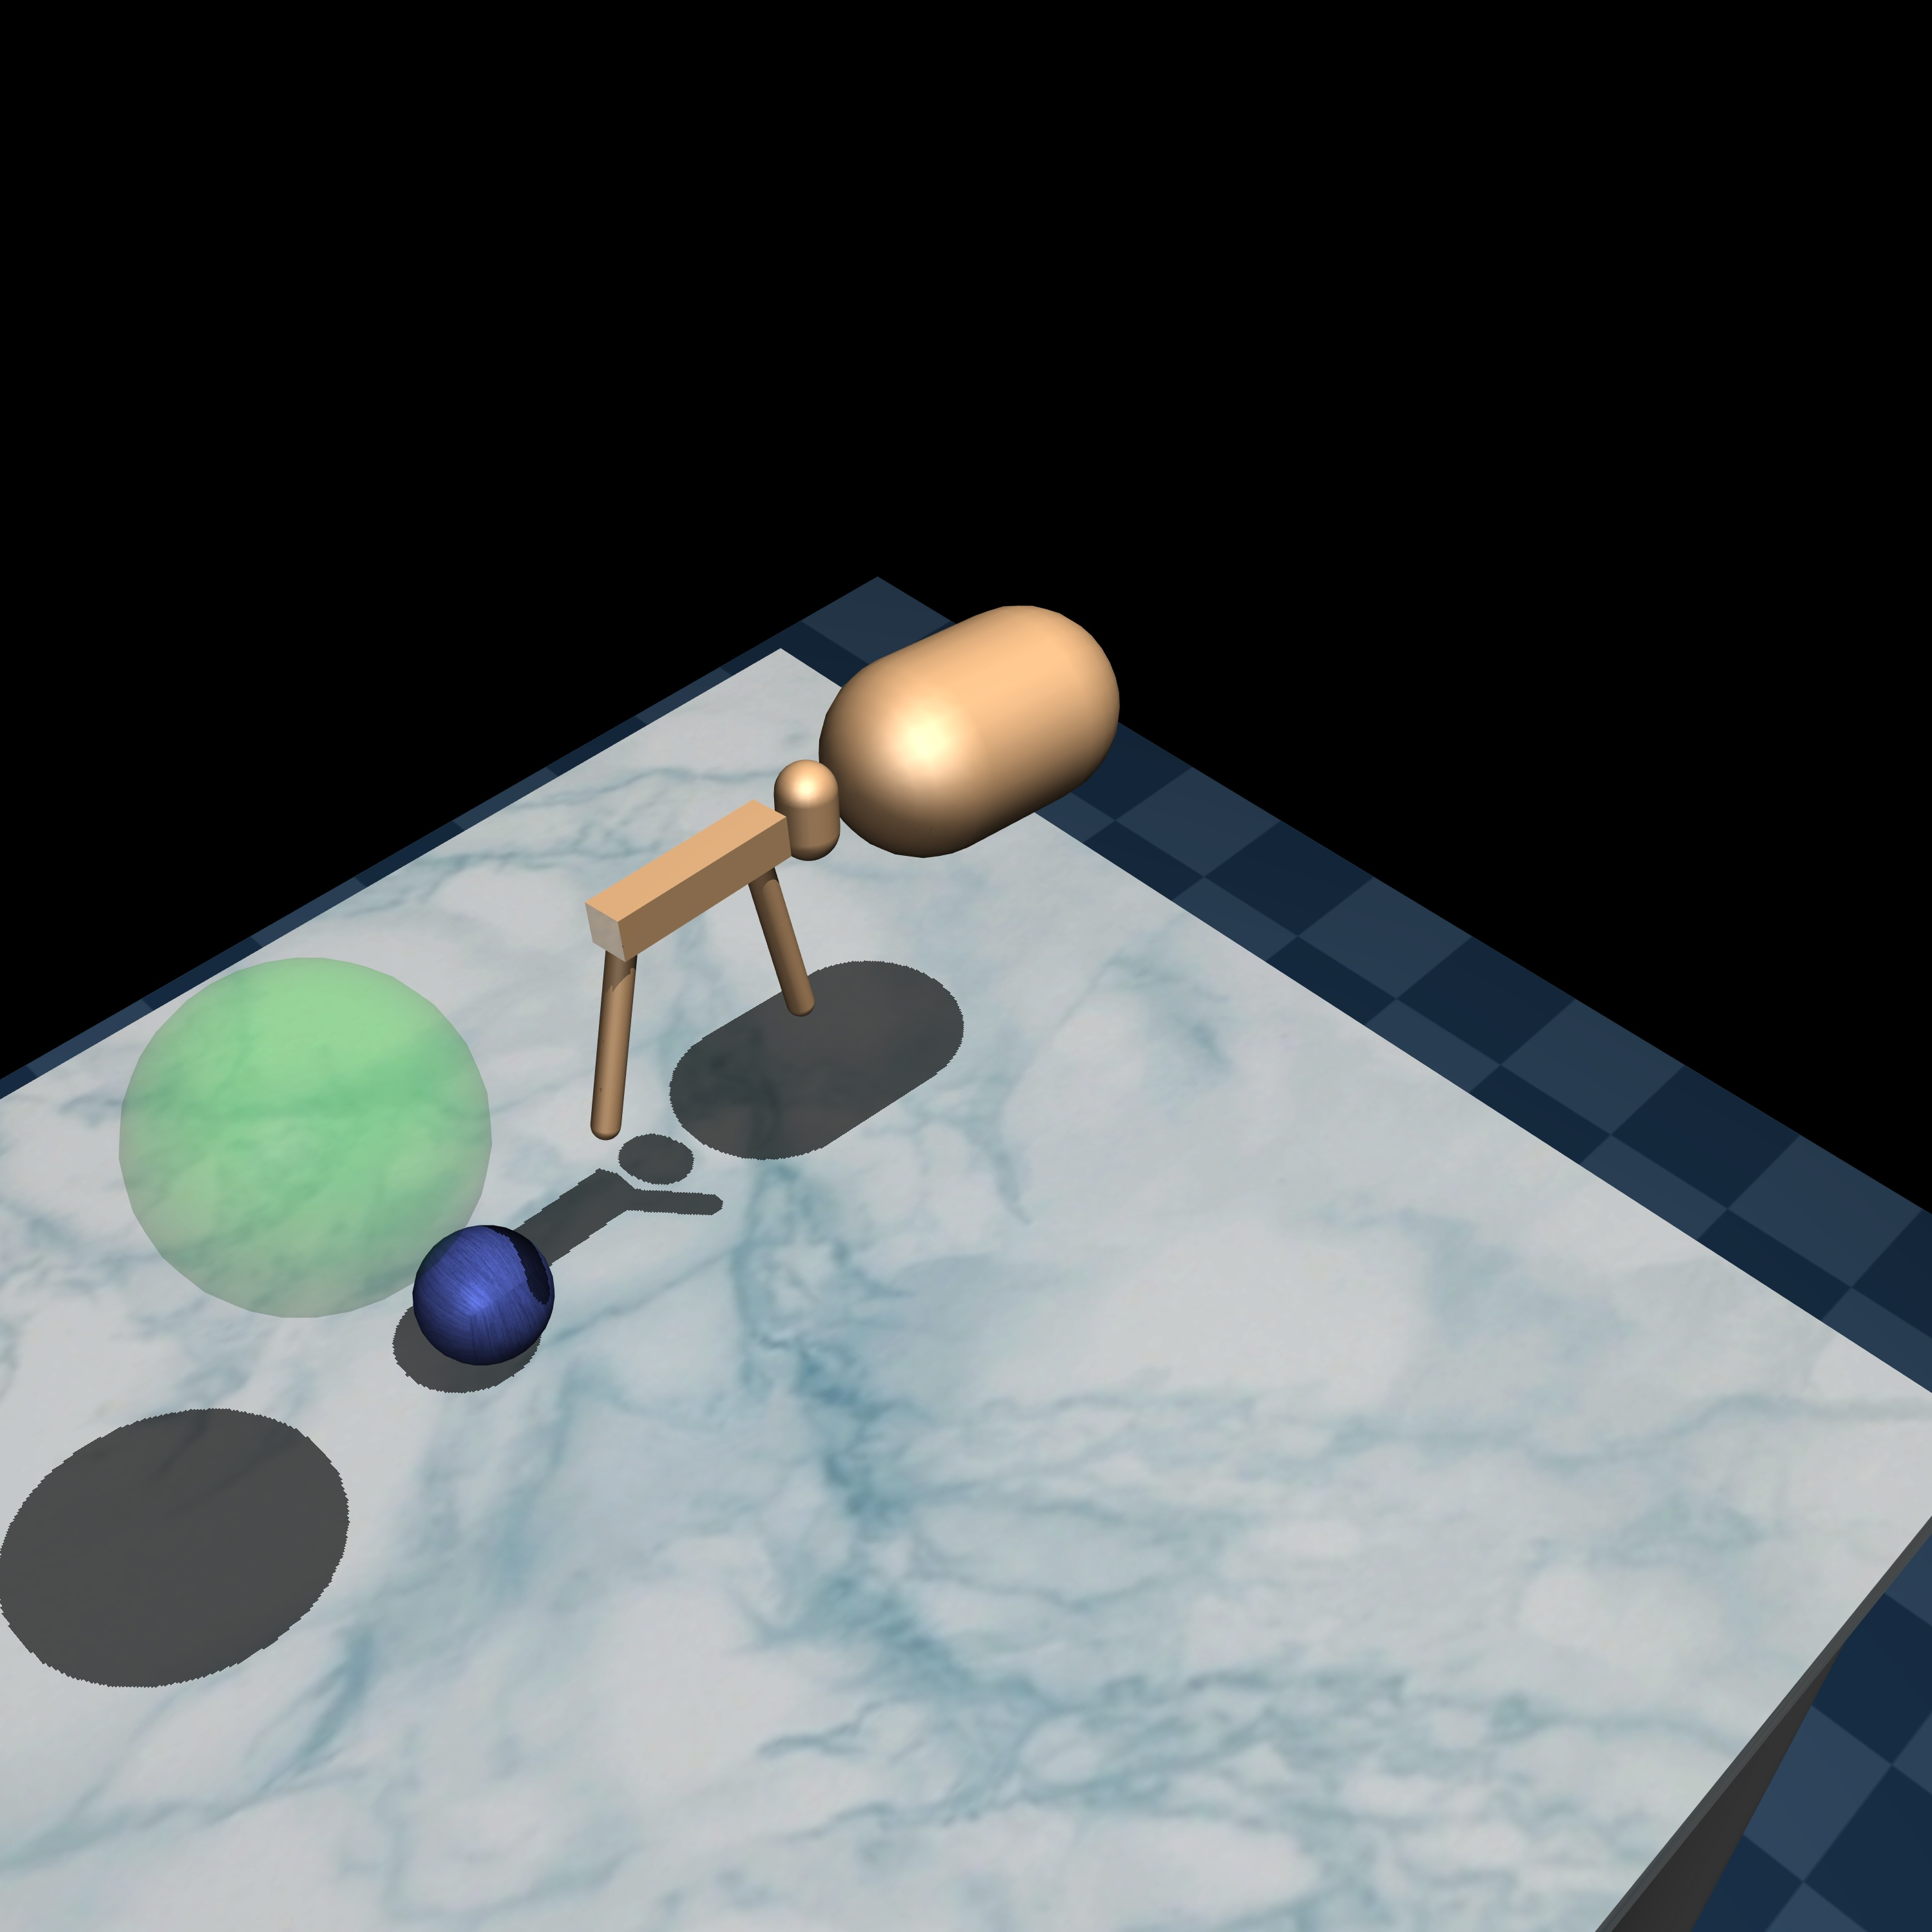
\includegraphics[width=\suppwidth\textwidth,valign=m]{Figures/supp/relocate/target/image-0015.jpg}
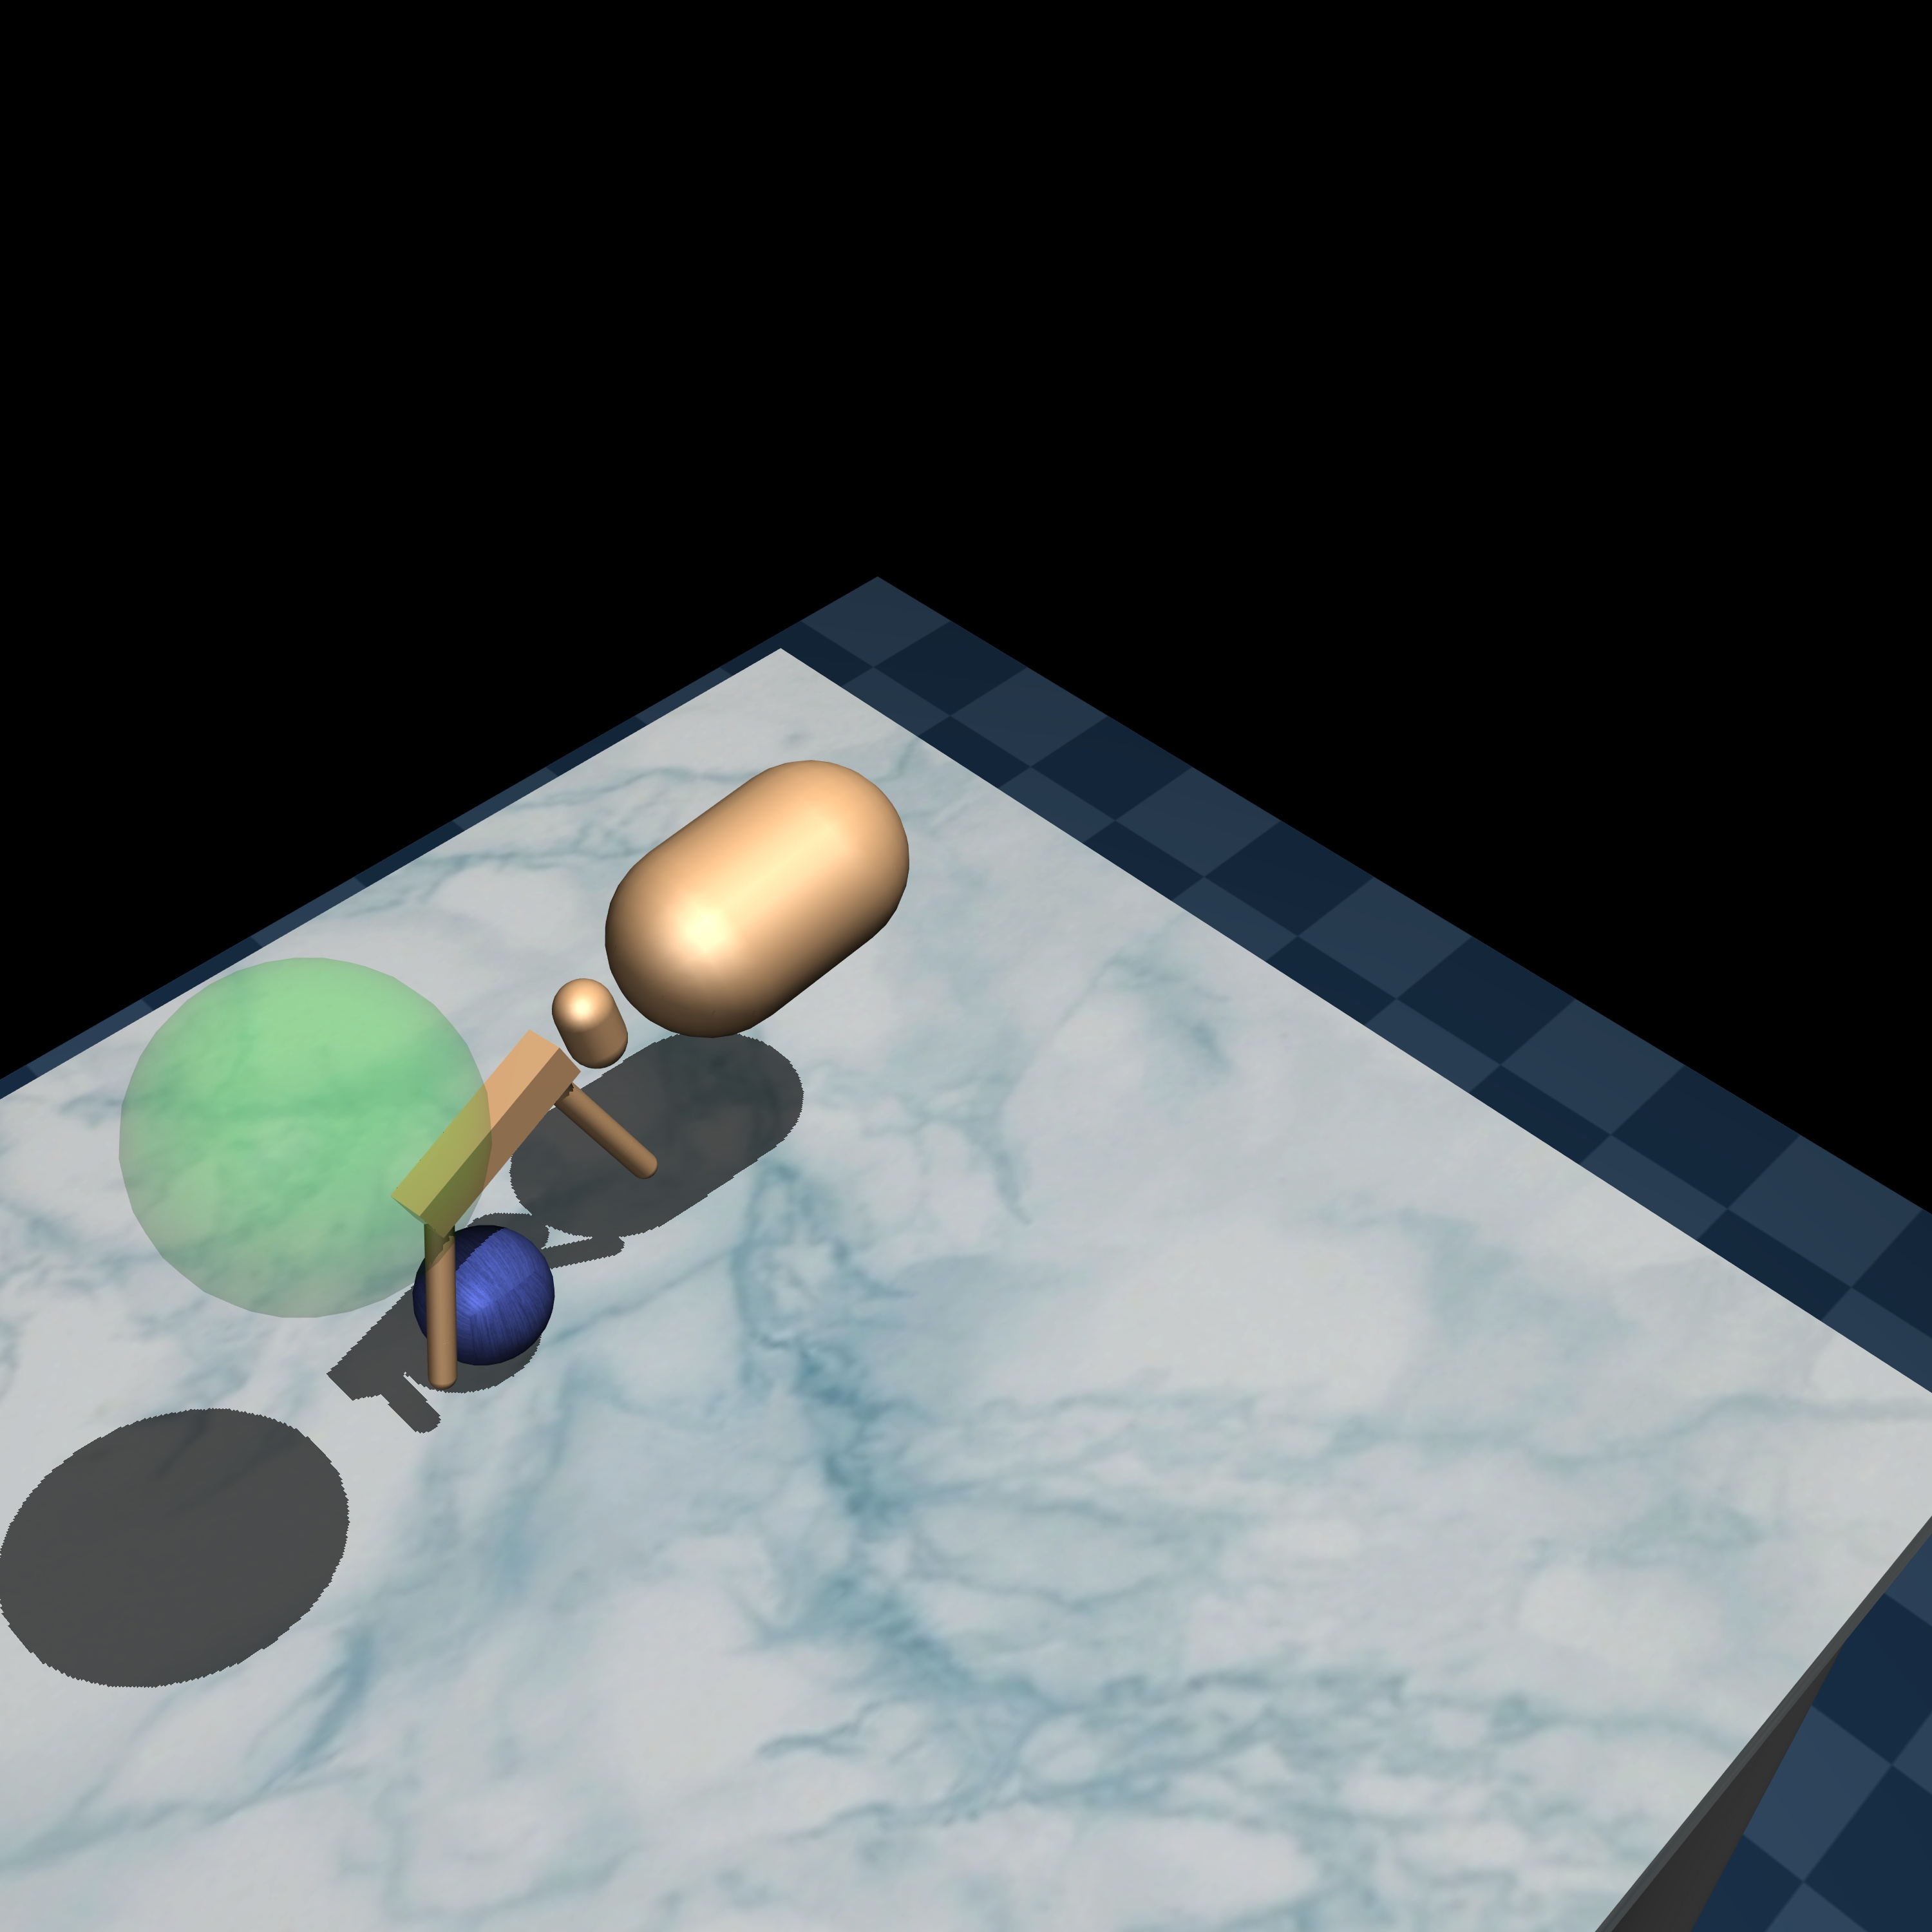
\includegraphics[width=\suppwidth\textwidth,valign=m]{Figures/supp/relocate/target/image-0024.jpg}
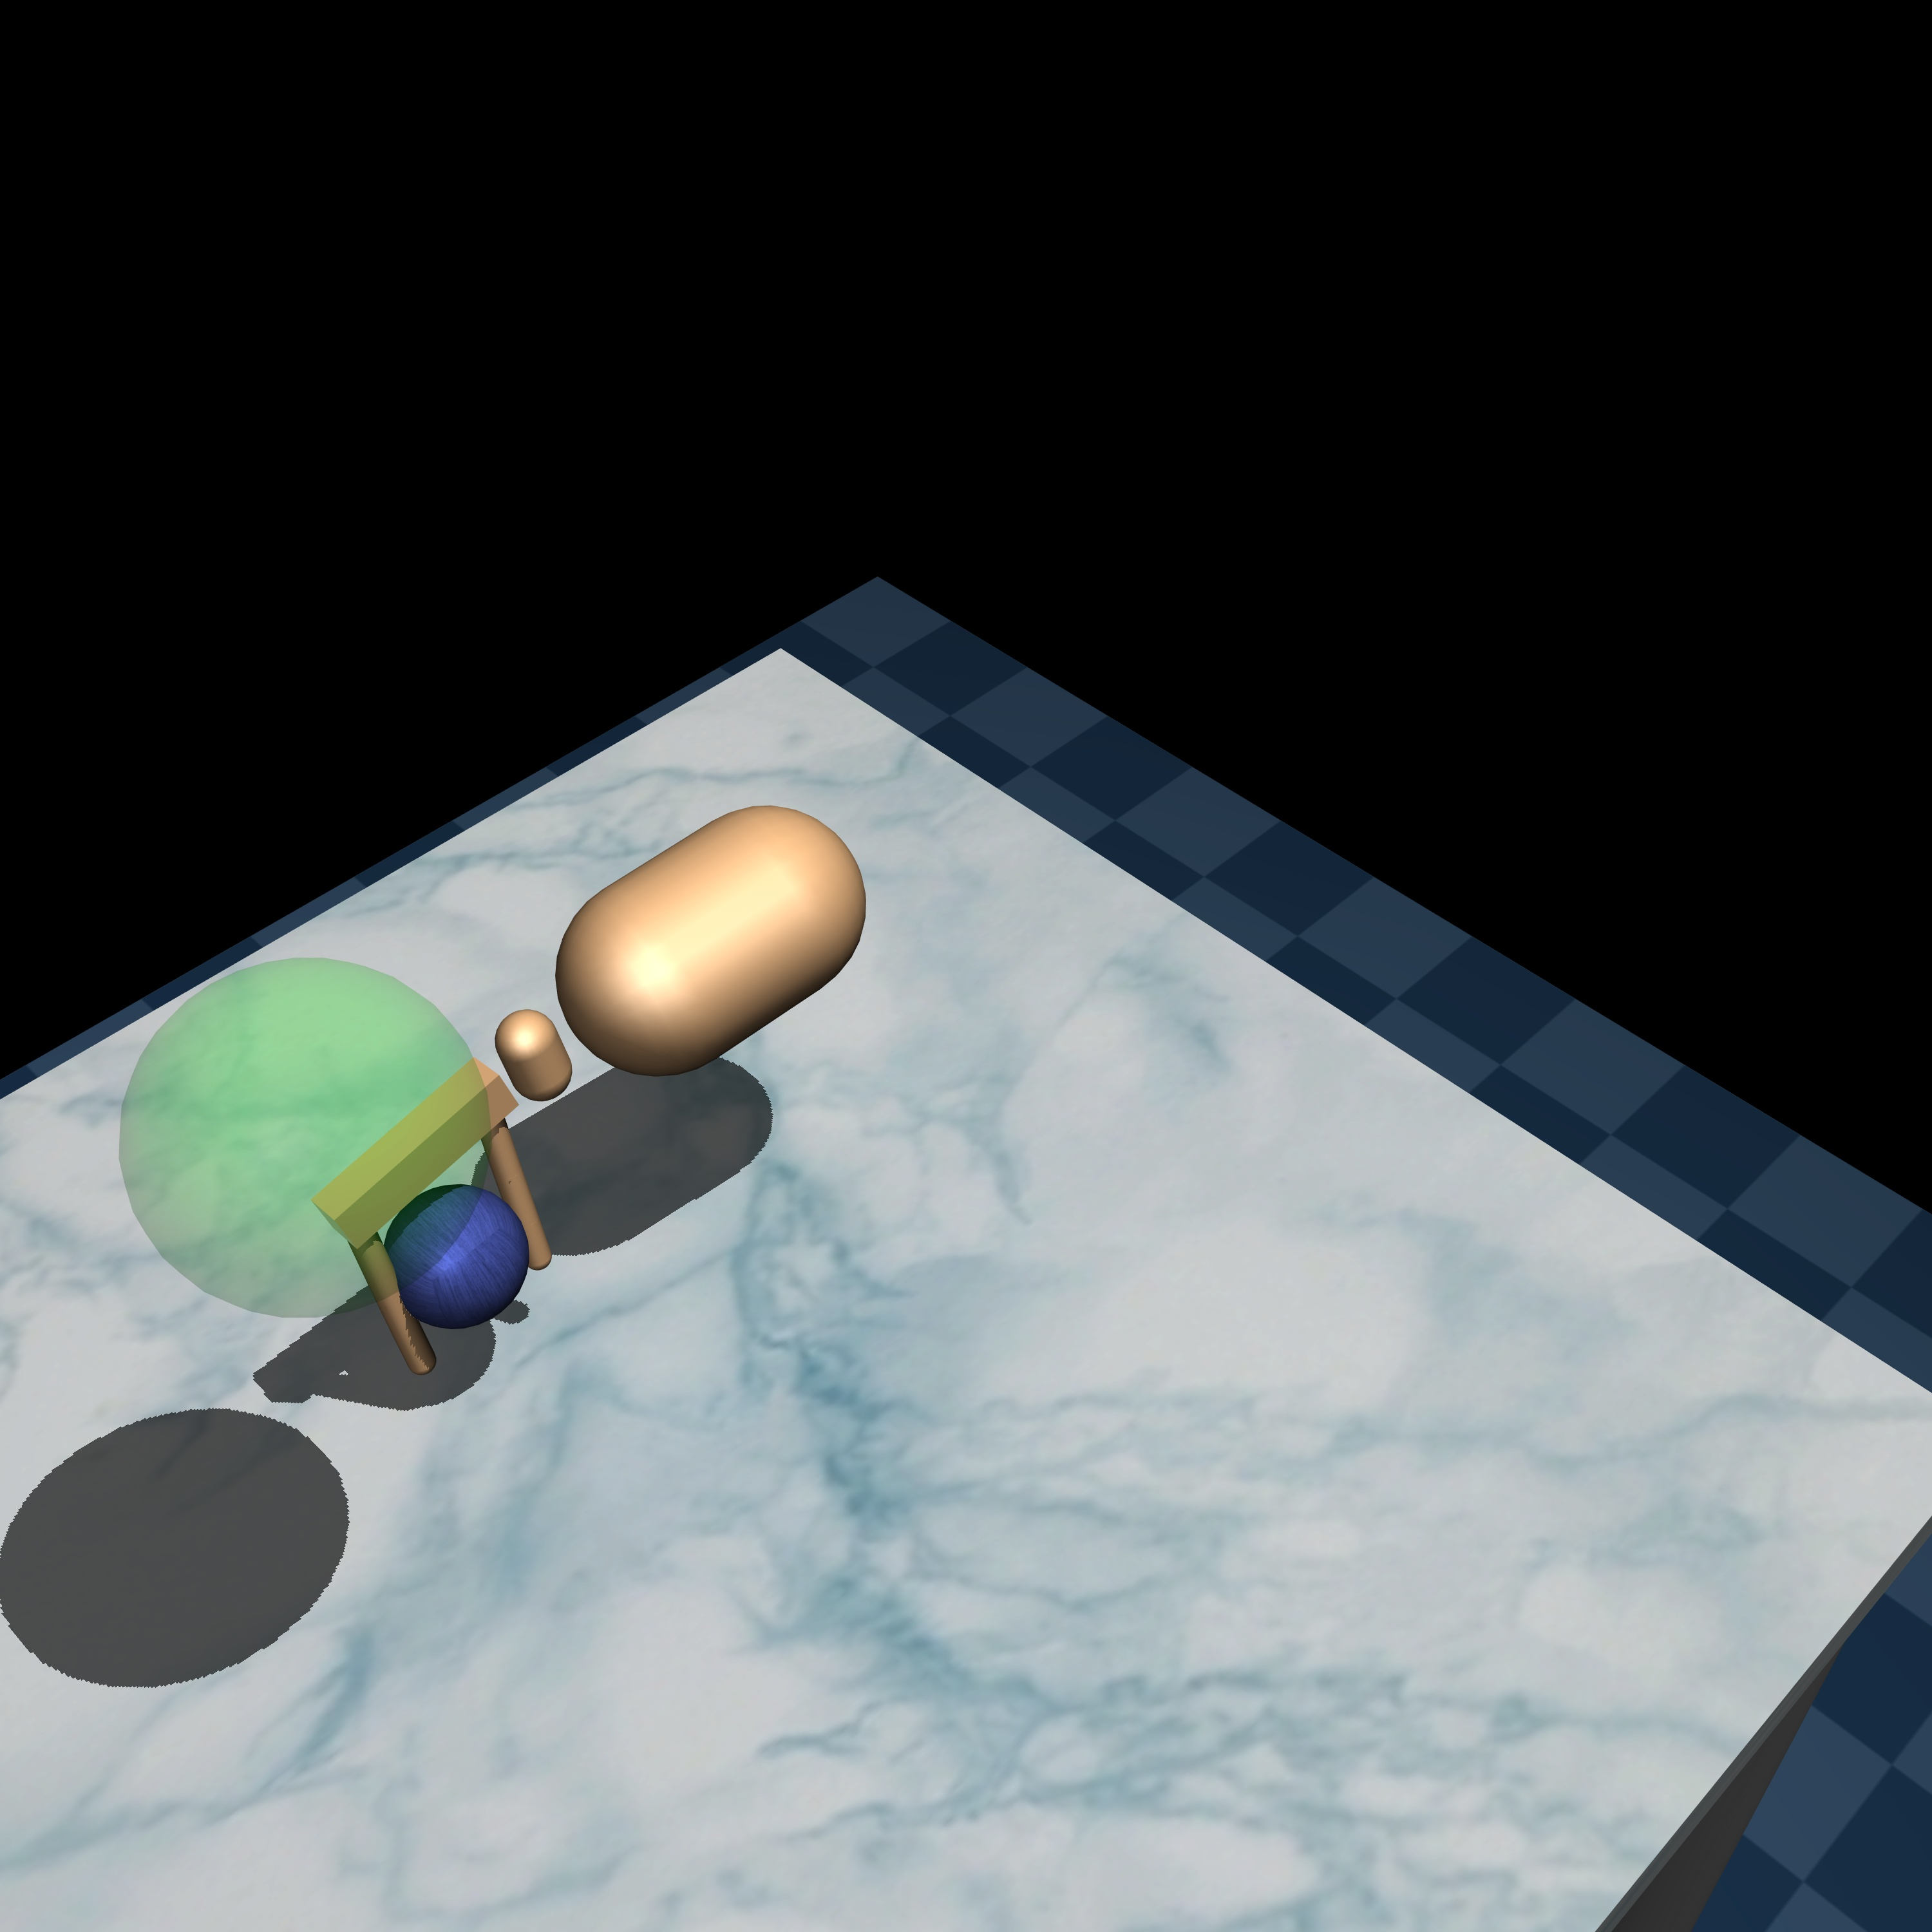
\includegraphics[width=\suppwidth\textwidth,valign=m]{Figures/supp/relocate/target/image-0033.jpg}
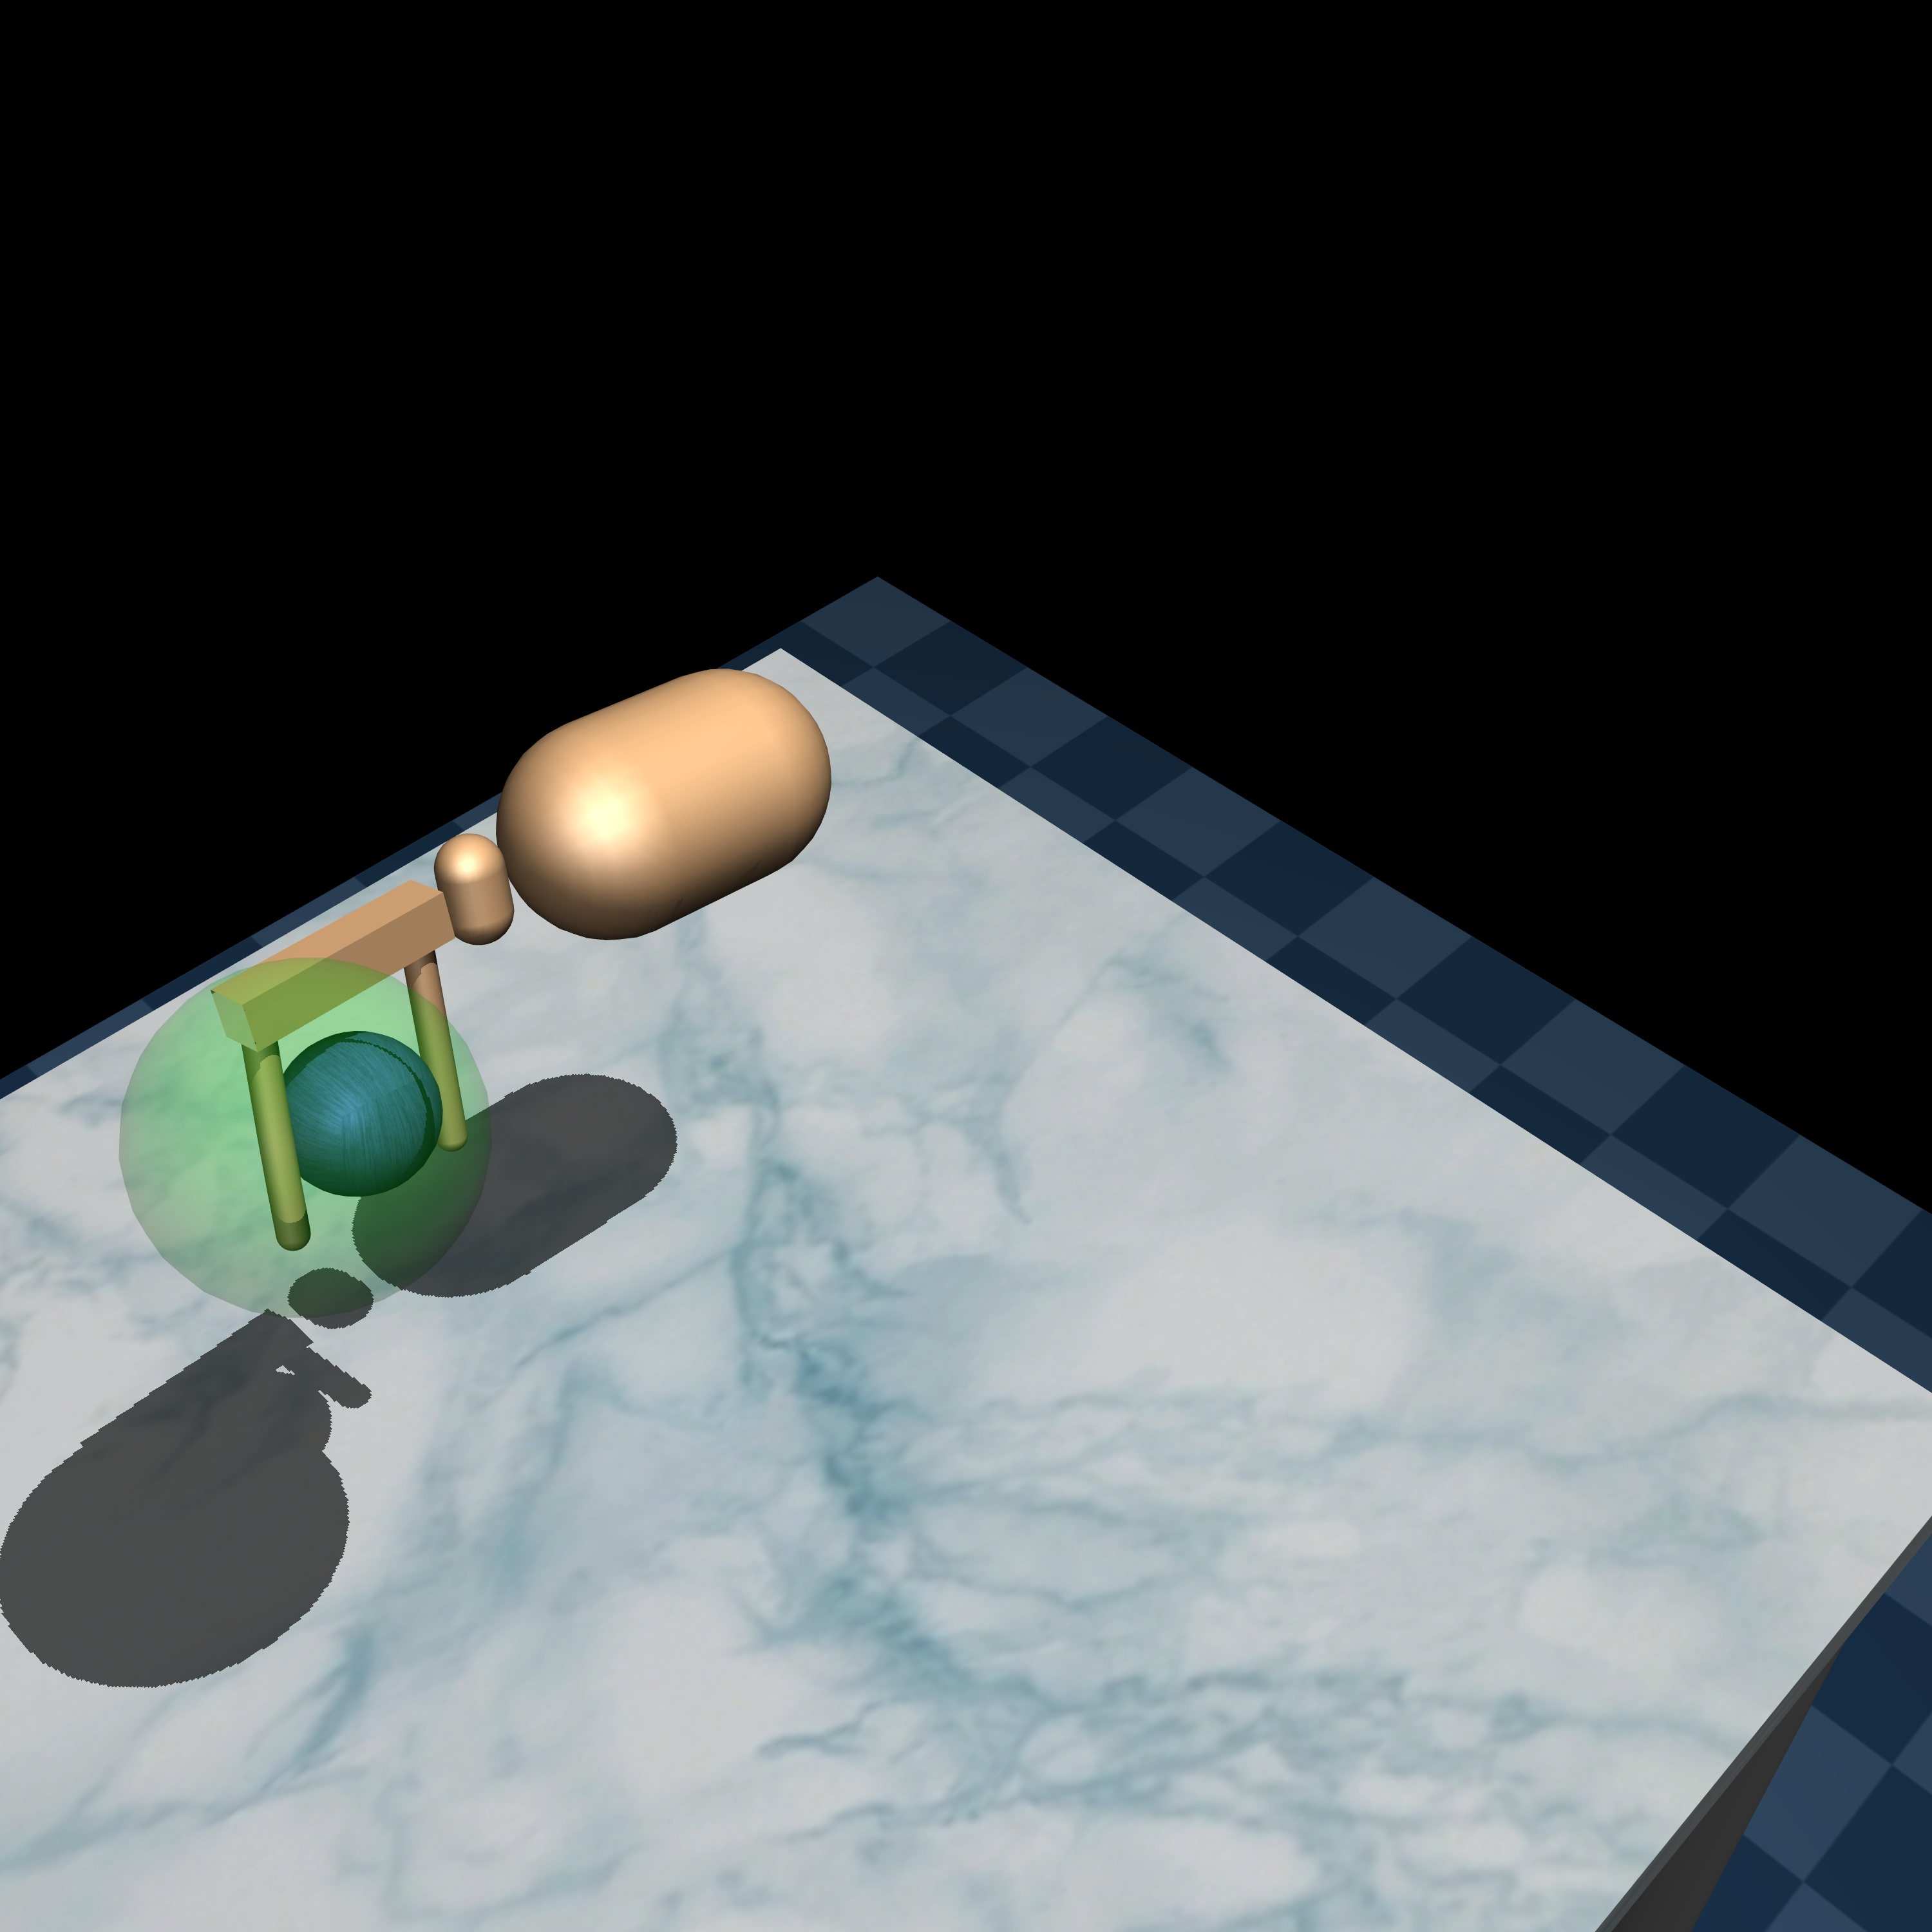
\includegraphics[width=\suppwidth\textwidth,valign=m]{Figures/supp/relocate/target/image-0042.jpg}
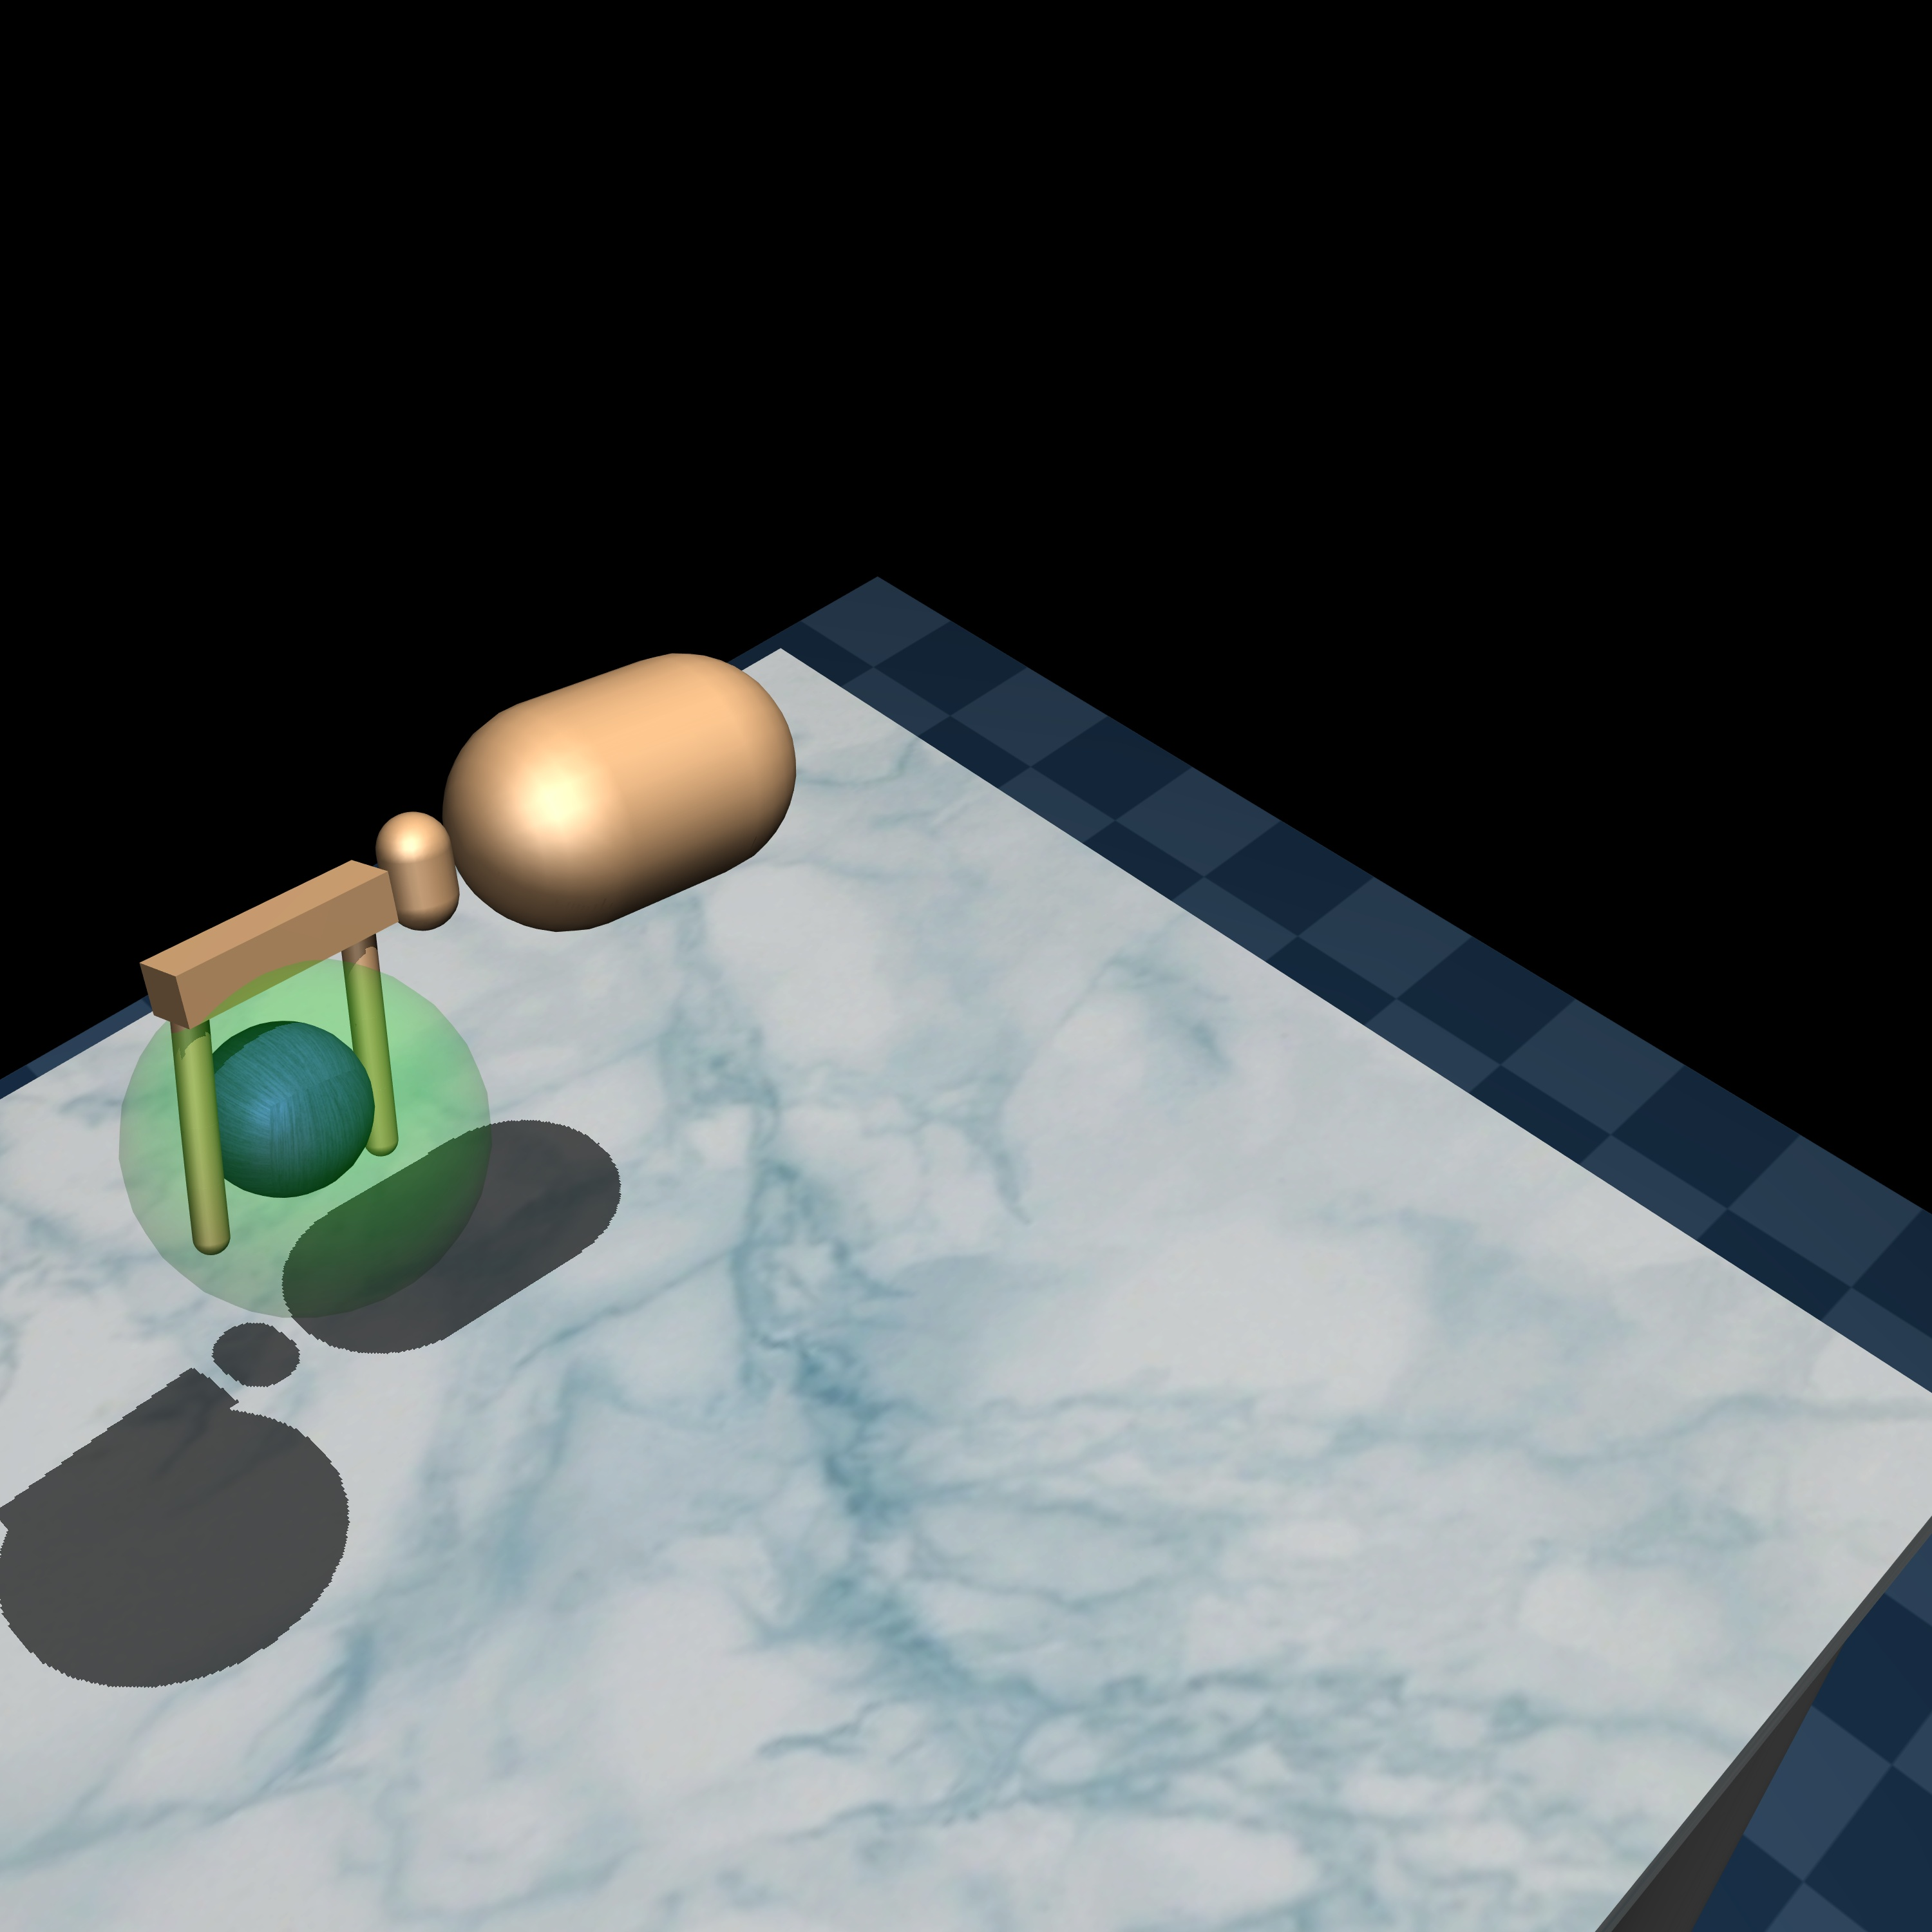
\includegraphics[width=\suppwidth\textwidth,valign=m]{Figures/supp/relocate/target/image-0051.jpg}
\end{tabular}
\vspace{-1ex}
\caption{\textbf{Qualitative results on the target robot on Hand Manipulation Suite tasks.}
We show the transferred policy on target robots.
The three rows shows  \texttt{Door}, \texttt{Hammer}, and \texttt{Relocate} tasks respectively.
From left to right in each row is a policy rollout on target robot at $\alpha=1$.
} 
\label{fig:dapg:policy:viz}
\end{figure}



